\documentclass
[a4paper,14pt,russian]{article}
\usepackage{extsizes}
\usepackage{cmap}     
\usepackage{mathtext}                       % для кодировки шрифтов в pdf
\usepackage{multirow}
\usepackage[T1, T2A, TS1]{fontenc}
\usepackage{paratype}
\usepackage[utf8]{inputenc}                  % для кодировки текста в UTF8
\usepackage[russian]{babel}
%\usepackage{pscyr}
\usepackage{textcomp}                            % красивые шрифты для кириллицы
\usepackage{url}
\urlstyle{rm} 
%\renewcommand{\rmdefault}{ftm}               % Times New Roman

% --- отступы по ГОСТу
\usepackage{geometry}
\geometry{left=2cm}
\geometry{right=1cm}
\geometry{top=2cm}
\geometry{bottom=2cm}

\usepackage{graphicx}                        % для вставки изображения
\graphicspath{{pics/}}                       % директория с изображениями (иначе не будет проставлять номера в ссылках)

\usepackage{amssymb,amsfonts,amsmath,amsthm} % математические дополнения от АМС
\usepackage{indentfirst}                     % отделять первую строку раздела абзацным отступом тоже
\usepackage[usenames,dvipsnames]{color}      % названия цветов 
\usepackage{ulem}                            % подчеркивания
\usepackage{array}

% --- полуторный интервал между строками
\usepackage{setspace}
\onehalfspacing

\setcounter{tocdepth}{3}                     % глубина просмотра уровней разделов для формирования оглавления
\setcounter{secnumdepth}{3}                  % глубина просмотра уровней разделов для их нумерации в оглавлении

\parindent=15mm                              % абзацный отступ
\renewcommand{\labelitemi}{--}               % задание маркера для первого уровня ненумерованных списков (тире)
\renewcommand*\labelenumi{\theenumi)}        % задание вида первого уровня нумерованных списков (цифра со скобкой)

\setcounter{secnumdepth}{5}	%нумерация  subsubsub - параграфа
%\renewcommand\contentsname{Оглавление}
%\renewcommand\large{\@setfontsize\large{15.5}{17}}
%\renewcommand\Large{\@setfontsize\Large{16.5}{19}}
%\renewcommand\theadfont{\normalsize}

\makeatletter
\renewcommand{\@biblabel}[1]{#1.} % Заменяем библиографию с квадратных скобок на точку:

%-----------------------------------------------------------------------------------------------------------------------



\begin{document}

%\thispagestyle{empty}

\begin{center}
Московский государственный технический университет \\ им. Н.Э. Баумана \\
\hrulefill
\end{center}

\vspace{8em}

\begin{center}
\large Дипломный проект \\ "Подсистема автономного опредления положения объектов"
\end{center}

\vspace{2em}
\thispagestyle{empty}

\begin{center}
\underline{\textbf{Техническое задание}} \\ (вид документа)
\end{center}

\begin{center}
\underline{\textbf{Бумага формата А4}} \\ (вид носителя)
\end{center}

\begin{center}
\underline{\textbf{7}} \\ (количество листов) %\arabic{page}
\end{center}

\vspace{2em}

\begin{flushright}
Выполнил: \\ студент группы ИУ5-129 \\ Жуков Р.В. \par\bigskip

Руководитель: \\ Терехов В.И.
\end{flushright}

\vspace{\fill}

\begin{center}
\hrulefill \\
Москва 2014
\end{center}

\newpage                          % Титульный лист
%\newpage

\section{Реферат}

                        % Реферат
                                         %
%\tableofcontents                         %
\section*{Введение}
В ходе создания подвижных автономных систем возникает задача организации ее навигации в пространстве. Данную задачу можно разделить на две:

\begin{itemize}
\item определение текущего местоположения объекта в пространстве;
\item прокладывание дальнейшего маршрута к точке назначения.
\end{itemize}
Данная работа посвещена решению первой задачи, так как она явлется первоочередной в построении системы навигации автономных систем.

Для определения текущего положения объекта можно использовать различные методы, основанные на глобальном позиционировании в географической системе координат с использованием позиционирования по спутникам (GPS, ГЛОНАСС), или методы, основанные на определении перемещения от стартовой позиции. При этом у данных методов разные сферы применения. Так, например, при позиционировании внутри помещения использование спутниковых систем позиционирвоания становиться невозможным по причине слабого сигнала или его полного отсутсвтвия, а так же из-за недостаточной точности в рамках навигации внутри интерьера помещения. Так же не стоит забывать про акутальность систем навигации в космической отрасли, где использование спутников является невозможным впринципе. 
Вторую группу методов принято называть методами одометрии, которые могут быть основаны на:
\begin{itemize}
\item на вращении колес;
\item использовании инерциальных измерительных приборов;
\item компьютерном зрении.
\end{itemize}

Каждый из них обладает своими плюсами и минусами \cite{odometryMethods}, но развитие вычислительной техники и алгоритмов компьютерного зрения дало мощный толчок к более широкому применению визуальной одометрии. Данный подход позволяет получать один видеоряд через видеокамеру и на его основе получать разные сведения об окружающей среде. Тем не менее он не лишен недостатков. Для борьбы с ними применяется комбинация нескольких методов одомтерии. 


\newpage

\section{Конструкторская часть}

\subsection{Разработка технического задания}
\subsubsection{Постановка задачи проектирования}

Целью разработки подсистемы автономного определения перемещения объекта является предоставления удобного с точки зрения интеграции компонента для встраивания во многие бытовые автономные автоматические системы,  в то же время дешевого и не требующего специализированных устройств для своей работы.

\subsubsection{Описание предметной области}
\paragraph{Естественно-языковое описание процесса.}

В ходе создания подвижных автономных систем возникает задача определения текущего местоположения объекта в пространстве.

Для этого можно использовать различные методы, основанные на глобальном позиционировании в географической системе координат с использованием позиционирования по спутникам (GPS, ГЛОНАСС), или методы, основанные на определении перемещения от стартовой позиции. При этом у данных методов разные сферы применения. Так, например, при позиционировании внутри помещения использование спутниковых систем позиционирвоания становиться невозможным по причине слабого сигнала или его полного отсутсвтвия, а так же из-за недостаточной точности в рамках навигации внутри интерьера помещения. Так же не стоит забывать про акутальность систем навигации в космической отрасли, где использование спутников является невозможным впринципе. 
Вторую группу методов принято называть методами одометрии, которые могут быть основаны на:
\begin{itemize}
\item на вращении колес;
\item использовании инерциальных измерительных приборов;
\item компьютерном зрении.
\end{itemize}

Каждый из них обладает своими плюсами и минусами \cite{odometryMethods}, но развитие вычислительной техники и алгоритмов компьютерного зрения дало мощный толчок к более широкому применению визуальной одометрии. Данный подход позволяет получать один видеоряд через видеокамеру и на его основе получать разные сведения об окружающей среде. Тем не менее он не лишен недостатков. Для борьбы с ними применяется комбинация нескольких методов одомтерии. 

Одним из вариантов сомещения методов является использование метода визуальной одометрии и инерционных измерительных устройств. 

При таком гибридном методе данные с видеокамеры и данные с инерционных измерительных устройств обрабатываются параллельно и независимо. В результате получаются два независимых рассчитынных положения носителя, после чего они сопоставляются, и из них выбираются наиболее правдоподобные. 

Таким образом, в процессе функционирования спроектированного модуля визуальной одометрии происходит следующий бесконечный процесс. 
На вход модуля непрерывно подается видео поток и данные об угловых скоростях и ускорении объекта относительно трех взаимноперпендикулярных осей. Эти данные обрабатываются параллельно в соответствующих модулях, на выходе каждого из которых получаем смещение объекта относительно предыдущего положения и его поворот. Далее эти данные совмещаются и выбираются наиболее правдоподобные, которые затем прибавляются к положению и углу поворота, высчитанным на предыдущей итерации. 


\paragraph{Графическое представление процесса}
Графическое представление процесса процесса представлено на рисунке~\ref{pic:predmetOblast}.

\begin{figure}[!htb]
\center{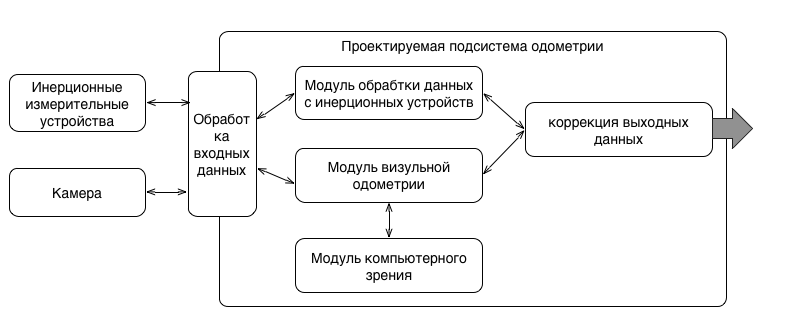
\includegraphics[width=0.8\linewidth]{pics/predmetOblast.png}}
\caption{Графическое представление процесса.}
\label{pic:predmetOblast}
\end{figure}

\paragraph{Вычисление оптического потока.}

\textbf{Оптический поток} — это изображение видимого движения объектов, поверхностей или краев сцены, получаемое в результате перемещения наблюдателя (глаз или камеры) относительно сцены\cite{wikiOpticalFlow}.

Существует несколько подходов к определению смещений между двумя соседними кадрами. Например, можно для каждого небольшого фрагмента (скажем, 8 на 8 пикселей) одного кадра найти наиболее похожий фрагмент на следующем кадре. В этом случае разность координат исходного и найденного фрагментов даст нам смещение. Основная сложность тут состоит в том, как быстро отыскать нужный фрагмент, не перебирая весь кадр пиксель за пикселем. Различные реализации этого подхода так или иначе решают проблему вычислительной сложности. Некоторые настолько успешно, что применяются, например, в распространенных стандартах сжатия видео. Платой за скорость естественно является качество. Мы же рассмотрим другой подход, который позволяет получить смещения не для фрагментов, а для каждого отдельного пикселя, и применяется тогда, когда скорость не столь критична. Именно с ним в литературе часто связывают термин “оптический поток”.

Данный подход часто называют дифференциальным, поскольку в его основе лежит вычисление частных производных по горизонтальному и вертикальному направлениям изображения. Как мы увидим далее, одних только производных недостаточно чтобы определить смещения. Именно поэтому на базе одной простой идеи появилось великое множество методов, каждый из которых использует какую-нибудь свою математическую пляску с бубном, чтобы достичь цели. Сконцентрируемся на методе Лукаса-Канаде (Lucas-Kanade), предложенном в 81 году Брюсом Лукасом и Такео Канаде. Данный метод является наименее ресурсоемким  \cite{habrOpticalFlowAbout} при этом обеспечивает приемлемое качество вычисления оптического потока. 

С математической точки зрения данный алгоритм можно описать следующим образом.
Пусть даны два изображения $F1$ и $F2$, и нам требуется найти смещение точки с координотой $x$. Рассматривая два последовательных изображения можно сказать:
$$ f_2(x) = f_1 (x-d)$$
Обратите внимание, что $f_1$ и $f_2$ при желании можно записать и в общем виде: $f_1(x) = I (x, y, t)$ ; $f_2(x) = I (x, y, t+1)$.

Свяжем известные значения со смещением d. Для этого запишем разложение в ряд Тейлора для $ f_1 (x-d)$:
$$  f_1 (x-d) =f_1(x) + df_1'(x) + O(d^2f_1'') $$
Предположим, что $ f_1 (x-d)$ достаточно хорошо аппроксимируется первой производной. Сделав это предположение, отбросим всё что после первой производной:
$$  f_1 (x-d) =f_1(x) + df_1'(x) $$

Смещение $d$ — это наша искомая величина, поэтому необходимо преобразовать $ f_1 (x-d)$ . Как мы условились ранее, $ f_2(x) = f_1 (x-d) $, поэтому просто перепишем:
$$ f_2(x)= f_1(x) - df_1'(x) $$
Отсюда следует:
$$ d = \frac{f_1(x)-f_2(x)}{f_1'(x)} $$

Следует отметить, что выше был рассмотрен одномерный случай и были сделаны несколько грубых допущений. Но описание алгоритма Лукаса-Канаде для двумерного случая только усложняет математические выводы и понимание сути. 

Для снижения погрешности вызванной отбрасыванием старших производных смещение для каждой пары кадров (назовём их $F_i$ и $F_{i+1}$) можно вычислять итеративно. В литературе это называется искажением (warping). На практике это означает, что, вычислив смещения на первой итерации, мы перемещаем каждый пиксель кадра $F_{i+1}$ в противоположную сторону так, чтобы это смещение компенсировать. На следующей итерации вместо исходного кадра $F_{i+1}$ мы будем использовать его искаженный вариант $F_{i+1}^1$. И так далее, пока на очередной итерации все полученные смещения не окажутся меньше заданного порогового значения. Итоговое смещение для каждого конкретного пикселя мы получаем как сумму его смещений на всех итерациях \cite{habrOpticalFlowTheory}.

Так же следует отметить, что данный алгоритм плохо работает на однотонных изображениях. Данный недостаток является самым критичным. 

\paragraph{Одометрия с использованием инерциальных измерительных устройств}
Навигационные решения надлежащего качества могут быть получены именно в результате взаимодействия или последующей совместной обработки данных от двух  источников - визуальной одометрии и инерциальной системы.  

В наиболее общей форме можно определить инерциальную систему как ортогональную триаду гироскопов и акселерометров, выполняющих непосредственные геопространственные измерения и вычислительный блок, осуществляющий алгоритмические преобразования данных непосредственных измерений.

Следует отметить, что гироскоп любого типа позволяет определять ориентацию в геодезическом пространстве в любой момент времени независимости от местоположения, скорости и других параметров носителя. Точность поставляемых гироскопом данных во всех случаях подвержена деградации («ухода») с течением времени. Величина «ухода» значительна и может составлять до нескольких градусов в час \cite{laserLocation}.

Акселерометры предназначены для измерения линейных ускорений. В равной степени они пригодны для измерений сил, так как согласно ньютоновской механике сила и ускорение есть разные проявления одного и того же физического явления.

В общем случае в системах навигации следует определять следующие показатели:
\begin{itemize}
\item \textbf{Рыскание} — угловые движения летательного аппарата, судна, автомобиля относительно вертикальной оси (см. также вертикальная ось самолёта), а также небольшие изменения курса вправо или влево, свойственные судну \cite{wikiRiskanie};
\item \textbf{Крен} — поворот объекта (судна, самолёта, фундамента) вокруг его продольной оси \cite{wikiKren};
\item \textbf{Тангаж} — угловое движение летательного аппарата или судна относительно главной (горизонтальной) поперечной оси инерции \cite{wikiTangazh}.

\end{itemize}
С учетом сделанных замечаний рассмотрим основные процедуры, выполняемые в навигационном комплексе на базисном уровне.

\textit{\textbf{Вычисление крена и тангажа посредством акселерометров}}

Обладая чувствительностью к земной гравитации, акселерометры обеспечивают измерение долговременных значений крена и тангажа по схеме, изображенной на рисунке~\ref{pic:tangazh}. Рассмотрим акселерометр, рабочая ось которого совпадает со строительной осью $oX$ носителя.

\begin{figure}[!htb]
\center{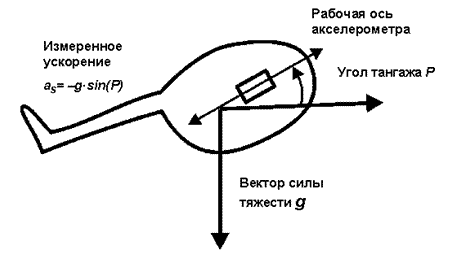
\includegraphics[width=0.6\linewidth]{pics/tangazh.png}}
\caption{Измерения величин крена и тангажа посредством акселерометров.}
\label{pic:tangazh}
\end{figure}

Полагая ускорение носителя равным нулю, мы можем вычислить угол тангажа как:
$$P = \arcsin (-a_s/g)$$

Аналогично вычисляется угол крена. Таким образом, два из трех углов, определяющих угловую ориентацию, могут быть определены только за счет использования акселерометров. Это совершенно очевидный результат, принимая во внимание то обстоятельство, что углы крена и тангажа по изначально определены по отношению к вертикали, которая в нашем случае соответствует вектору тяжести. Однако, здесь следует признать, что описанный метод не может быть использован на практике сам по себе, так как в описанной схеме существенно состояние покоя, в котором должна находиться система. Если это условие не соблюдается, то совершенно очевидно, что отсутствует принципиальная возможность выделить вектор ускорения свободного падения из суммы всех ускорений, которую испытывает система.

\textit{\textbf{Вычисление изменений ориентации с использованием гироскопов}}

Как отмечено выше, в конструкции навигационного комплекса используются оптические гироскопы, обладающие чувствительностью к изменениям ориентации т.е. к величине угловой скорости. Интегрирование (численное суммирование) значений, измеренных гироскопами, обеспечивает определение кратковременных угловых перемещений в физическом пространстве.

Для корректного расчета угла поворота должны быть учтены
внутренние ошибки гироскопа – дрейф, ошибка масштабного коэффициента, случайный шум.

При этом внутренние ошибки  гироскопа полностью смешаны с истинными значениями и не могут быть отделены от них на базисном информационном уровне. В процессе дальнейшей обработки эта смесь подвергается интегрированию, в результате чего возникает ошибочное угловое смещение, которое, таким образом, приобретает долговременный характер (рис. ~\ref{pic:acell}). Точная оценка величины ошибочного углового смещения и его устранение осуществляется при генерации навигационного решения на последующем навигационном уровне.

\begin{figure}[!htb]
\center{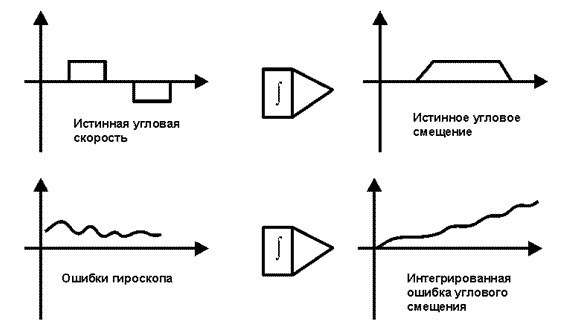
\includegraphics[width=0.6\linewidth]{pics/acelerometr.png}}
\caption{Схема определения углового смещения.}
\label{pic:acell}
\end{figure}

\textit{\textbf{Определение координат пространственного положения с помощью акселерометров.}}

Наличие акселерометров позволяет определять величины линейных ускорений, которые испытывает система. Положим, что ориентация системы в физическом пространстве определена точно с помощью методов, описанных выше. Тогда имеется возможность выделить вектор силы гравитации среди всей суммы векторов сил, приложенных к системе и, следовательно, оценить величину ускорения. Численное интегрирование ускорения позволяет перейти к скорости, а повторное интегрирование к перемещению. Таким образом, с учетом представленных выше замечаний и правилах перехода из физического пространства в географическое, появляется принципиальная возможность оценить геодезические координаты системы в любой момент времени.

\paragraph{Корректировка выходных данных}

\paragraph{Анализ функций, подлежащих автоматизации}

\subsubsection{Выбор критериев качества}
Выделим основные критерии, по которым следует оценивать разрабатываемую подсистему.
\begin{itemize}
\item \textbf{Необходимость в специальном оборудовании} - исходя из задачи, предполагается использование проектируемого модуля в низкобюджетных системах. В связи с этим необходимо обеспечить корректную работу подсистемы с неспециальным оборудованием таким, как бытовые камеры. 
\item \textbf{Стоимость необходимого оборудования} – исходя из предыдущего пункта, следует обеспечивать поддержку наиболее дешевого оборудования. 
\item \textbf{Сложность интеграции} – в современном мире наличия многих конкурентов и налогов одним из ключевых факторов при выборе между ними является простота использования продукта. В связи с этим необходимо снизить время, необходимое на интеграцию с разрабатываемой подсистемой, путем предоставления удобного в использовании API.
\item \textbf{Точность} - данный критерия является важным для задач определения положения в пространстве априори, так как при низкой точности использование систем данного рода становится бесмысленным. Тем не менее в рамках многих задач обеспечение чрезмерно высокой точности является избыточным.
\item \textbf{Возможность свободного использования} – нередко разработчики программных или аппаратных продуктов накладыают ограничение в виде разного рода лицензий распространения, которые ограничивают пользователей в распространении и использовании своих продуктов. В связи с этим важным явлется свободность использования продукта в любых целях, не  противоречящих законодательству стран, где проихсходит его использование.
\end{itemize}

\subsubsection{Анализ аналогов и прототипов}


\paragraph{Сравнительный анализ}

Для сравнения представленных вариантов воспользуемся методом взвешенной суммы. Данный метод позволяет объединить ряд критериев сравнения в один интегральный показатель, по которому затем выбирается наилучший вариант, соответствующий максимальному значению этого интегрального показателя. Метод взвешенной суммы можно представить следующим образом: 
$$ Y = \max_{j \ni m} \displaystyle\sum_{i=1}^{n} \alpha_i \cdot K_{ij},$$
где $\sum_{i=1}^{n} \alpha_i = 1$

По этому критерию проводится сравнение $j (j = 1, 2, …, m)$ вариантов по $i (i = 1, 2, …, n)$ показателям, где:

$n$ – количество показателей сравнения;

$m$ – количество вариантов сравнения.

$K_{ij}$ – нормированный коэффициент соответствия $i$-ого параметра $j$-ого варианта эталонному значению, т.е. для $j$-ого варианта:
$$ K_{ij} = \frac{\max_{j} X_{ij}} {X_{ij}}, $$
$$ 0 < K_{ij} < 1 $$
Соответствие систем-аналогов выбранным критериям качества представлено в Таблице

\subsubsection{Перечень задач, подлежащих решению в процессе разработки}

Исходя из приведенного выше первичного анализа предметной области можно сформировать список задач, подлежащих решению.

Необходимо решить следующие задачи:

\begin{enumerate}
\item разработка структуры и архитектуры подсистемы системы; 
\item разработка требований к формату и структуре передаваемых данных;
\item разработка алгоритмов обработки информации;
\item выбор и обоснование КТС, необходимого для реализации системы;
\item разработка графа диалога и набора экранных форм;
\item оценка предполагаемого качества функционирования системы;
\item организационно-экономическое обоснование разработки;
\item рекомендации по охране труда.
\end{enumerate}





\subsection{Проектирование подсистемы}
\subsubsection{Разработка структуры подсистемы}
\paragraph{Определение состава компонентов}

Исходя из анализа функций структурно в подсистеме можно выделить следующие основные части:
\begin{itemize}
\item \textbf{модуль обработки входных данных} (преобразует входные данные в удобоваримый вариант для последующей обработки);
\item \textbf{модуль компьютерного зрения }(позволяет обрабатывать изображения и производить их анализ для построения визуальной одометрии);
\item \textbf{модуль визуальной одометрии} (высчитывает перемещение и угол поворота камеры на основе последовательности изображений);
\item \textbf{модуль обработки данных с инерционных приборов} (производит математическую обработку показаний датчиков и на ее основе вычисляет перемещение объекта);
\item \textbf{модуль сопоставления  и вывода данных} (сравнивает показания двух предыдущих модулей и на их основе выводит наиболее правдоподобное положение объекта).
\end{itemize}

\paragraph{Определение структуры компонентов}
Согласно общепринятой терминалогии система состоит из подсистем, а те в свою очередь из модулей. Таким образом разрабатываемая подсистема состоит из следующих модулей:

\begin{itemize}
\item обработки входных данных;
\item обработки выходных данных;
\item визульной одометрии;
\item компьютерного зрения;
\item настроек;
\item одометрии на основе инерционных устройств.
\end{itemize}

Графически архитектура подсистемы представлена на рисунке~\ref{pic:acrhitec}.

\begin{figure}[!htb]
\center{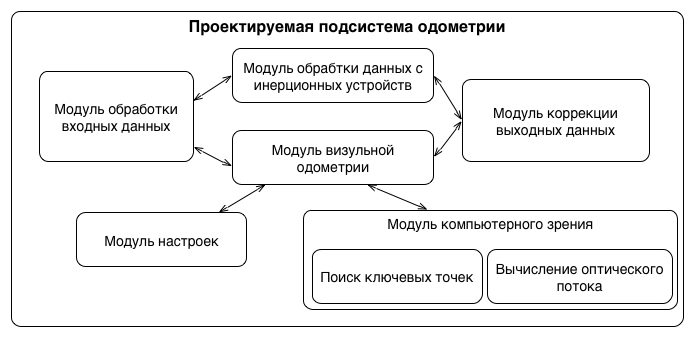
\includegraphics[width=0.8\linewidth]{pics/achitecture.png}}
\caption{Структура компонентов.}
\label{pic:acrhitec}
\end{figure}

\textbf{Назначение модулей}

\begin{itemize}
\item \textbf{Модуль обработки входных данных} - нормализует входные данные и аккумулирует их, в случае слишком высокой частоты их поступления.
\item \textbf{Модуль обработки выходных данных} - сравниевает данные, полученные независимо в модуле визуальной одометрии и в модуле обработки данных с ИИУ, и принимает решение об их корректности на основе определенных сигнальных показателей (см. пункт~\ref{item:outputCorrect}).
\item \textbf{Модуль визуальной одометрии} – вычисляет перемещения на основе видеоряда. Для обработки видео использует модуль компьютерного зрения. 
\item \textbf{Модуль компьютерного зрения} – реализует стандартные алгоритмы компютеного зрения, такие как вычисление оптического потока, поиск опорных точек на изображении, трансформация и измениние изображений.
\item \textbf{Модуль одометрии на основе инерционных устроств} – производит расчеты перемещения обхекта на основе полученных данныз с гироскопов и акселерометров.
\item \textbf{Модуль настроек} - содержит в себе данные об используемом оборудовании и его характеристиках. Эти данные используются в модулях одометрии. 
\end{itemize}

\paragraph{Описание процессов}
В ходе работы всей подсистемы протекает множество процессов по обработке и преобразованию информации. Выделим ключевые из них.

\textbf{Визуальная одометрия.}

В данной работе делается упор на создание визуальной одометрии на основе одной бытовой камеры и относительно слабых вычислительных устройств. Такое решение требует соблюдения двух условий, которые приемлемы при создании большинства современных мобильных роботов:
\begin{enumerate}
\item перемещение происходит по земле или другой горизонтальной плоскости;
\item камера жестко закреплена относительно самого носителя.
\end{enumerate}

При соблюдении этих условий работу визуальной одометрии можно описать в 8 шагов\cite{visaulOdometryMy}.
\begin{enumerate}
\item Исправление изображения для исключения искажения линз.
\item Вычисление оптического потока для кадра.
\item Проверка полученных векторов смещения, исключение движущихся в кадре объектов, исключение ошибочных векторов.
\item Разделение всего оптического потока на две части: «наземную» и «небесную».
\item В «небесной» части перейти к цилиндрической системе координат и высчитать угол поворота относительно двух последних кадров, определяя тем самым угол поворота $\theta$.
\item В «наземной» части выделить векторы $(u,v)$ из оптического потока  и вычислить перемещение в плоскости x-y , получив вектор $(x, y)$.
\item Прибавить $(x, y, \theta)$ к изначальному положению объекта $(X, Y, \Theta)$, получив новое положение объекта.
\item Перейти к шагу 1 для следующего кадра. Периодически обновлять ключевые точки.
\end{enumerate}
	
В общем виде процесс вычисления оптического потока представлен на рисунке~\ref{pic:visOdometryProc}.

\begin{figure}[!htb]
\center{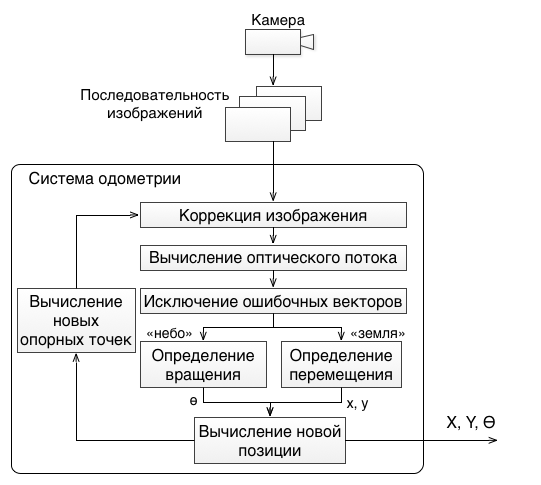
\includegraphics[width=0.8\linewidth]{pics/visualOdometryProcess.png}}
\caption{Графическое представление процесса визуальной одометрии}
\label{pic:visOdometryProc}
\end{figure}

\textbf{Обработка данных с инерционных измерительных устроств.}

Обработка данных с инерционных устройств представляет собой несколько операций интегрирования полученных данных. 
Рассмотрим переход от ускорений к перемещению.

Пусть на выходе акселерометра снимаются ускорения $Z_a$, $Y_a$ и $Z_a$, которые показывают ускрения по осям $X$, $Y$, $Z$.

Как мы знаем из курса физики, $ \int_a^b a(t)dt = V(t)+C $.
В то же время $ \int_a^b V(t)dt = S(t)+C $. Таким образом получаем:
$$
\iint_a^b a(t)dt = \int_a^b V(t) + C_v = S(t) + C_v \cdot t + C_s 
$$.

Так как $С_s$ в нашем случае, это начальное положение носителя, то его мы принимаем = 0. Отсюда получаем формулу:
$$
\iint_a^b a(t)dt = \int_a^b V(t) + C_v = S(t) + C_v \cdot t .
$$

Однако все упрощается, если период замеров настолько мал, что ускорение можно считать равномерным. Тогда формулы преобретают следующий вид:
$$ V_t = V_{t-1} + a_t \cdot t$$
$$ S_t = S_{t-1} + V_t \cdot t $$

Графически это можно выразить тремя графиками (рис.~\ref{pic:integral}): показывающими рассчитанное значения пермещения и сокрости в зависимости от времени. 

\begin{figure}[!htb]
\center{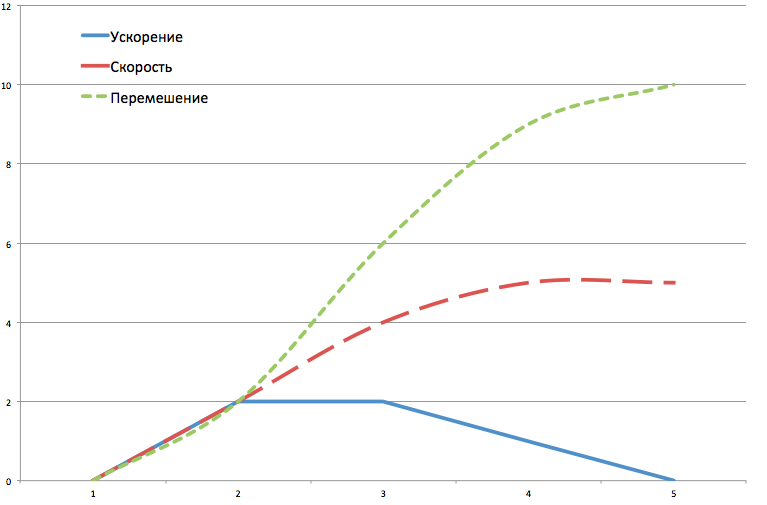
\includegraphics[width=0.8\linewidth]{pics/integrals.png}}
\caption{Пример интегрирования ускорения для получения перемещения}
\label{pic:integral}
\end{figure}


Производя подобные математические вычисления для координат $X$ и 
$Y$ получаем перемещения по этим координатам. Причем мы можем опускать финальную константу интегрирования, так как нам необходимо определить не пройденный путь от начала движения, а именно путь, пройденный за последнний временной отрезок. 

Аналогично обрабатываются данные с акселерометров, с одинм лишь отличием - акселерометры могут предоставлять сразу угловую скорость, что позволяет производить лишь одно интегрирование.


\paragraph{Математическое обеспечение}\label{math}

В рамках данной работы многие процессы основываются на фундаментальных исследованиях в области компьютерного зрения и обработки изображений. Далее рассматриваются основные из них.

\textbf{Поиск ключевых точек}

Есть много видов местных ключевых точек, которые можно отслеживать. Для начала стоит рассмотреть что из себя представляет ключевая точка сама по себе (ключевая особенность изображения). Очевидно, что если мы выбираем точку на большой однотонной стене, то будет не легко найти, что же точку в следующем кадре из видео.

Если все точки на стене могут быть одинаковыми или даже очень похожи, то у нас будет мало шансов отслеживания этой точки в последующих кадрах. С другой стороны, если мы выберем точку, которая является уникальной, то у нас будут довольно хорошие шансы снова найти эту точку. На практике, точка или черта, которая мы выбираем в качестве клюевой должны быть уникальным или почти уникальны, и должна быть параметризуемой таким образом, чтобы ее можно было отличить от других точек на изображении.

Возвращаясь к нашей аналогии с большой пустой стеной, мы могли бы попытаться искать точки, которые имеют некоторые значительные изменения в окрестности, например, большую производную. На практике оказывается, что этого не достаточно. Точка, в которой большое значение производной, может находиться на какой-то линии, но все точки на этой линии будут иметь такую же или близкую производную.

Однако, если высокие значения производные наблюдаются в двух ортогональных направлениях, то можно надеяться, что эта точка будет уникальной. По этой причине, такие особенности на изображении называются углами. Очевидно, углы - не края - это точки, которые содержат достаточно информации, чтобы ее нашли на последующих кадрах.

Определение углов опирается на матрице производных второго порядка 
$(\partial^2 x, \partial^2 y, \partial x \partial y)$ интенсивностей изображения. Эта терминология происходит от матрицы Гессе вокруг точки, которая определяется в двух измерениях следующим образом:

$$ 
H(p) = 
\begin{bmatrix} 
	\frac{\partial^2 I}{\partial x^2} & \frac{\partial^2 I}{\partial x \partial y}  \\ 
 	 \frac{\partial^2 I}{\partial x \partial y} & \frac{\partial^2 I}{\partial y^2} 
\end{bmatrix}
$$

Такие углы, по определению Харриса, места на изображении, где автокорреляционная матрица вторых производных имеет два больших собственных значения. По сути, это означает, что есть текстуры или грани , идущие, по крайней мере, в двух отдельных направлениях, сосредоточенные вокруг такой точки, так же, как реальные углы имеют по крайней мере два ребра, сходящихся в точку. Использование вторых производных позволяет точно определить особенности, потому что они не отвечают единым градиентами(так как при первой производной равной константе, вторая будет равна нулю). Это определение имеет дополнительное преимущество, в том, что когда мы рассматриваем только собственных значений автокорреляционной матрицы, мы рассматриваем величины, инвариантные также к вращению, что является важным, потому что объекты, которые мы отслеживаем могут вращаться, а также перемещаться. Следует также отметить, что эти два собственных значения делают больше, чем просто определяют, является ли точка перспективной для обслеживания - они также обеспечивают идентифицирующую роль для точки.

В используемом в данной работе пакете компьютерного зрения используется функция  $cvGoodFeaturesToTrack()$.
\begin{verbatim}
void cvGoodFeaturesToTrack(
        const CvArr* image,
        CvArr* eigImage, CvArr* tempImage,
        CvPoint2D32f* corners,
        int* cornerCount,
        double qualityLevel,
        double minDistance,
        const CvArr* mask=NULL,
        int blockSize=3,
        int useHarris=0,
        double k=0.04 
);
\end{verbatim}
Эта функция вычисляет воторые производные для точек и их собственные значения. Результатом работы функции является список точек, которые являются хорошими кандидатами для ключевых точек.

\textbf{Оптический поток}

Задача вычисления оптического потока можно сформулировать следующим образом: оценить движение между двумя кадрами не имея никакой информации о происходящем, кроме самих кадров\cite{OpenCVBook}. 

Вычисля оптический поток, мы можем связать для каждого пикселя определить некий ветктор смешения, которые будут показывать куда переместился пиксель между предыдущим кадром и текущим кадром. Такой  подход обычно называют плотным оптическим потоком, который определяет перемещение каждого пикселя. Метод Хорн-Шунка (Horn-Schunck) вычисляет именно такой оптический поток. В его основе лежит один, казалось бы, простой принцип - просто пытаться найти наиболее похожий пиксель на следующем кадре в пределах какого-то окна вокруг исходного пикселя.

На практике расчет плотного оптического потока затруднителен. Рассмотрим движение белого листа бумаги. Многие из белых пикселей в предыдущем кадре просто остаются белыми на следующих. Изменения будут лишь на границах листа, и то, только вокруг гарниц перпендикулярных движению. В результате необходимо прибегать к различным математическим приемам, что сказывается на увеличении ресурсоемкости операции в целом. 

Это приводит нас к альтернативному варианту, выборочный оптического потока. Алгоритмы такого рода опираются на некоторые средства определения заранее подмножество точек, которые должны быть отслежены. Если эти точки имеют определенные свойства, такие как свойства ключевых особенностей, обсуждаемые ранее, тогда отслеживая будет относительно точным и надежными. Для многих практических случаев, вычислительная стоимость выборочного оптичкского потока намного меньше, чем у плотного оптического потока, поэтому последнему отводится только академический интерес.

Рассмотрим наиболее популярный метод вычисления выборочного оптического потока - метод Лукаса-Канаде (Lucas-Kanade). Этот метод также имеет реализацию, которая работает с пирамидами изображений, что позволяет нам отслеживать быстрые движения. В данной работе используется именно он, так как он обладает наиболее низкой вычислительной сложностью. 

{\large \textit{\textbf{Метод Лукаса-Канаде}}}
\label{label:lucas-kanade-math}
Метод (алгоритм) Лукаса - Канаде (ЛК) создавался в 1981 году и первоначально задумывался для вычисления плотного оптического потока. Тем не менее, Алгоритм работал и с любым количеством точек для отлеживания, что позволило использовать его в столь важных выборочных оптических потоках. 

Алгоритм ЛК может быть применен для определнного числа точек, потому что он опирается только на локальной информации о точке, которая является производной в некотором маленьком окне вокруг каждой из ключевых точек. Недостатком использования небольших локальных окон в ЛК является то, что большие смещения могут перемещать точки за пределы таких локального окон, что приведет к невозможности их нахождения. Эта проблема привела к разработке "пирамидальной" версии алгоритма, которая составляет пирамиду из нескольких копий изображения разного размера, после чего вычисляет оптический поток, начиная с самого высокого уровня в пирамиде изображений, постепенно опускаясь по уровням для более высокой точности. 

\begin{figure}[!htb]
\center{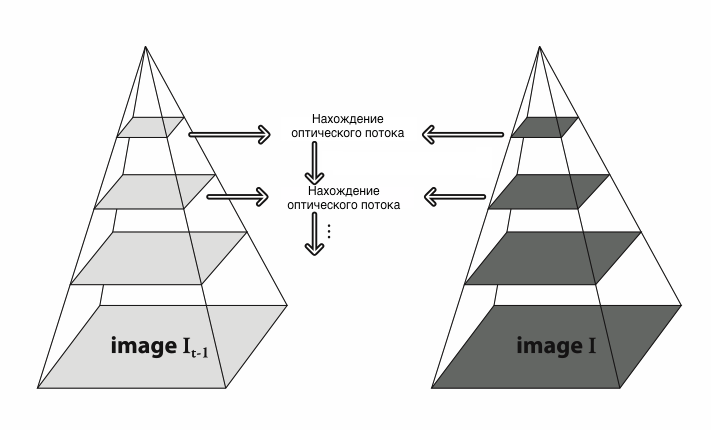
\includegraphics[width=0.8\linewidth]{pics/pyrLK.png}}
\caption{Графическое представление работы "пирамидальной" версии алгоритма ЛК}
\label{pic:pyrLK}
\end{figure}

\textbf{Принцип работы алгоритма}

Основная идея алгоритма ЛК основывается на трех предположениях. 
\begin{enumerate}
\item \textit{Яркость постояна.} Предполагается, что пиксель не меняет внешний вид, переходя от кадра к кадру. Для изображений в градациях серого (для случая с цветными изображениями есть более строгое допущение, но оно сводится к этому) это означает, что яркость пикселя не меняется, при его отслеживании от кадра к кадру. 
\item \textit{Малые сдвиги}. Изображение двигается медленно во времени. На практике это означает, что объект от кадра к кадру сдвигается незанчительно.
\item \textit{Пространственная когерентность.} Соседние точки в кадре принадлежат к одной и той же поверхности и имеют аналогичные смещения.
\end{enumerate}

Из первого допущения следует:
$$
f(x, t) \equiv I(x(t), t) = I(x(t+dt), t + dt)
$$

Отсюда следует, что интенсивность отслеживаиваемых пикселей не измененяется с течением времени:
$$
\frac{\partial f(x)}{\partial t} = 0
$$

Второе предположение, по существу, означает, что движения от кадра к кадру крайне малы. Другими словами, мы можем рассматривать это изменение как аппроксимацию производной от интенсивности по времени. Чтобы понять последствия этого предположения, рассмотрим сначала случай одного пространственного измерения.
Запишем уравнение яркости $F(x,t)$ с учетом зависимости $x$ от $t$ и применим правило частного дифференцирования:
$$
\underbrace{\frac{\partial I }{\partial x} \Bigr|_t}_{I_x} 
\underbrace{\left( \frac{\partial x }{\partial t} \right)}_{V} + 
\underbrace{\frac{\partial I }{\partial t} \Bigr|_{x(t)}}_{I_t} =
 0,
$$

где $I_x$ является пространственной производной по первому изображению, $I_t$ это производная между изображениями в течение долгого времени, и $V$ -скорость, которую мы ищем. Таким образом, мы приходим к простому уравнению для скорости оптического потока в простой одномерной случае:

$$ V = \frac{I_t}{I_x} $$

Рассмотрим стандартную задачу в одномерном случае. На рисунке~\ref{pic:OptFlow1D} представлена ее графическая иллюстрация. Кривая $I(x, t)$ изображает некую грань, слева от которой значения интенсивности высоки, а справа - низкие. Необходимо определить как сдвинулась это грань на следующем кадре. 

\begin{figure}[!htb]
\center{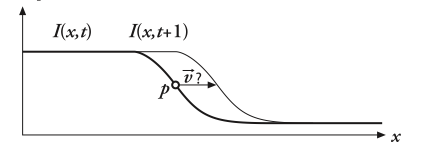
\includegraphics[width=0.8\linewidth]{pics/optFlow1D.png}}
\caption{Графическое представление задачи нахождения оптического потока в одномерном случае.}
\label{pic:OptFlow1D}
\end{figure}

На рисунке~\ref{pic:OptFlow1DSolve} показано как можно решить такую задачу. При учете двух первых предположений  получим следующее:
$$
I_x = \frac{\partial I}{\partial x} \Bigr|_t \; и \;
I_t = \frac{\partial I}{\partial t} \Bigr|_{x=p} \Rightarrow 
\vec{V} \approx - \frac{I_t}{I_x}
$$
\begin{figure}[!htb]
\center{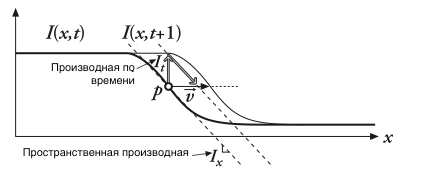
\includegraphics[width=0.8\linewidth]{pics/OptFlow1DSolve.png}}
\caption{Графическое представление решения задачи нахождения оптического потока в одномерном случае.}
\label{pic:OptFlow1DSolve}
\end{figure}

Теперь рассмотрим двумерный случай. Будем обозначть $u_y$ скорость вдоль оси $Y$, а $u_x$ -вдоль $X$:
$$ I_xu +I_yv+I_t = 0 \equiv 
\frac{\partial I}{\partial t} + 
u_x \cdot \frac{\partial I}{\partial x} + 
u_y \cdot \frac{\partial I}{\partial y} = 0 
$$

Полученное уравнение, говорит нам о том, что сумма частных производных должны быть равна нулю. Но вознакает проблема - уравнение у нас одно, а неизвестных в нем два: $u_x$ и $u_y$.

Воспользовавшись третьим предположением, о том, что соседние пиксели смещаются на одинаковое расстояние, запишем это же уравнение для окна 5х5 пикселей, получив 25 уравнений. Очевидно, что 3 допущение не всегда верно, поэтому в общем случае система не имеет решения поэтому перейдем к минимизации ошибки:

$$
E(u_x, u_y) = \sum \limits_{i,j} g(x_i, y_i) 
\left[ \frac{\partial I}{\partial t} + 
u_x \cdot \frac{\partial I}{\partial x} + 
u_y \cdot \frac{\partial I}{\partial y} \right]^2
$$

Здесь $g$ — это функция, определяющая весовые коэффициенты для пикселей. Самые распространенный вариант — двумерная гауссиана, которая дает наибольший вес центральному пикселю и все меньший по мере удаления от центра (см. рис.~\ref{pic:Gaussian2d}).

\begin{figure}[!htb]
\center{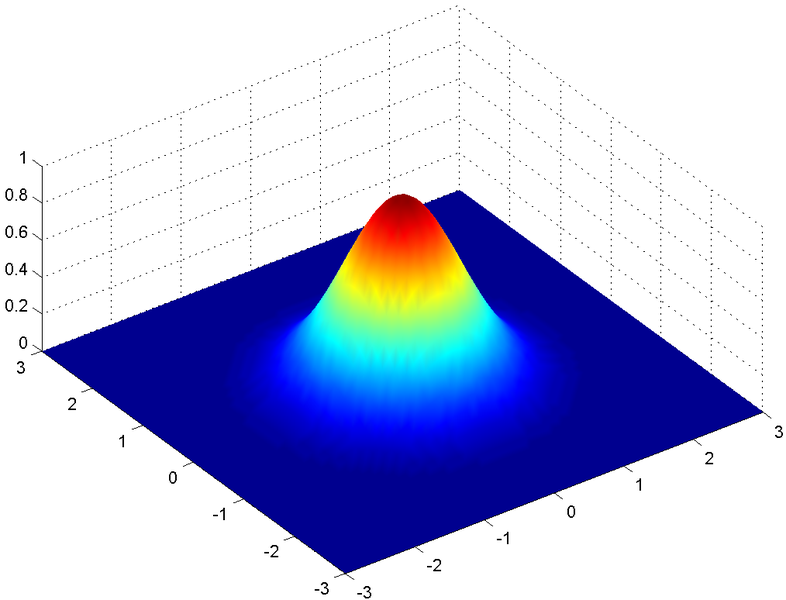
\includegraphics[width=0.8\linewidth]{pics/Gaussian2d.png}}
\caption{Двумерная гауссиана}
\label{pic:Gaussian2d}
\end{figure}

Чтобы найти минимум  $E(u_x, u_y)$ воспользуемся методом наименьших квадратов, найдем её частные производные по $u_x$ и $u_y$ и запишем в более компактной форме, приравням к 0:

$$
\frac{\partial E(u_x, u_y) }{\partial u_x} = 
\sum \limits_{i,j} g(x_i, y_i) 
\left[
u_x \left( \frac{\partial I}{\partial x} \right)^2 +
	u_y \frac{\partial I}{\partial y}\frac{\partial I}{\partial x} +
	\frac{\partial I}{\partial x}\frac{\partial I}{\partial t}
\right] = 0
$$

$$
\frac{\partial E(u_x, u_y) }{\partial u_y} = 
\sum \limits_{i,j} g(x_i, y_i) 
\left[
	u_x \frac{\partial I}{\partial y}\frac{\partial I}{\partial x} +
	u_y \left( \frac{\partial I}{\partial y} \right)^2 +
	\frac{\partial I}{\partial x}\frac{\partial I}{\partial t}
\right] = 0
$$

Перепишем эти два уравнения в матричной форме:
$$ M \vec{u} = \vec{b}$$

Где: 
$$ M = 
\left[ 	
\begin{array}{cc}
	\sum \limits_{i,j} g(x_i, y_i) 
		\left( \frac{\partial I}{\partial x} \right)^2 
	& \sum \limits_{i,j} g(x_i, y_i) 
			\frac{\partial I}{\partial x} 										\frac{\partial I}{\partial y} 
	\\ 
	\sum \limits_{i,j} g(x_i, y_i) 
			\frac{\partial I}{\partial x} 										\frac{\partial I}{\partial y} 
	& \sum \limits_{i,j} g(x_i, y_i)
		\left( \frac{\partial I}{\partial y} \right)^2 
\end{array} 
\right]
$$

$$
\vec{b} = -
\left[ 	
\begin{array}{c}
\sum \limits_{i,j} g(x_i, y_i) 
			\frac{\partial I}{\partial t} 										\frac{\partial I}{\partial x}  \\ 
\sum \limits_{i,j} g(x_i, y_i) 
			\frac{\partial I}{\partial t} 										\frac{\partial I}{\partial y}
\end{array} 
\right]
$$

$$
\vec{u} = 
\left[ 	
\begin{array}{c}
  u_x\\ 
	u_y
\end{array} 
\right]
$$

Если матрица М обратима (имеет ранг 2), можем вычислить $u_x$ и $u_y$ , которые минимизируют ошибку $E$\cite{habrOpticalFlowAbout}:
$$
\widehat{u} = M^{-1} \cdot \vec{b}
$$

\textbf{Калибровка камеры}
Еще одиним математическим аспектом данной работы является калибровка камеры. 

\textit{\textbf{Калибровка камеры}} — это задача получения внутренних и внешних параметров камеры по имеющимся фотографиям или видео, отснятым ей\cite{wikiCalibrate}.

Рассмотрим простейшую модель камеры, камеры-обскуры. В этой простой модели, свет рассматривается в качестве потка от сцены или удаленного объекта, но только один луч попадает из любой конкретный точки этого объекта. Все эти точки проецируются на матрицу камеры или другую поверхность изображения. В результате, изображение на этой плоскости изображения всегда в фокусе, а масштаб изображения относительной его раельного размера определяется одним параметром камеры -  ее фокусным расстоянием. На рисунке~\ref{pic:cameraModel} схематично показана рассматриваемая модель камеры\cite{OpenCVBook}. 

\begin{figure}[!htb]
\center{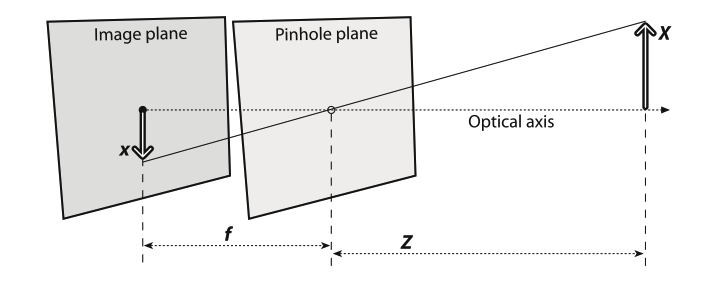
\includegraphics[width=0.8\linewidth]{pics/cameraModel.png}}
\caption{Модель камеры-обскуры}
\label{pic:cameraModel}
\end{figure}

Из изображения видно, что, на основе подобия треугольников, $-x/f = X/Z$:
$$	-x = f \cdot \frac{X}{Z} $$

Учитывая тот факт, что главная оптическая ось пересекает плоскость изображения не в координате $(0,0)$, в координате $с$ получим:

\begin{equation}
\label{formula:focus}
-x = f \cdot \frac{X}{Z} + с
\end{equation}

Далее будем рассматривать именно цифровые камеры с ПЗС-матрицами. У данных камер есть одна особенность - пиксели матрицы не квадратной формы из-за технологических условий изготовления. Учитывая этот факт, распишем уравнение (\ref{formula:focus}) для координат $x$ и $y$:

$$ u = f \cdot s_u \cdot \frac{X}{Z} + c_u $$
$$ v = f \cdot s_v \cdot \frac{X}{Z} + c_v $$

где $s_u$ и $s_v$ - коэффициенты формы пикселя.
Запишем эти уравнения в матричной форме:

\begin{equation}
\label{formula:matrixProection}
q = \frac{1}{Z} \cdot M \cdot Q
\end{equation}

где 
$Q_i = 
\left( 
\begin{array}{c}
X_i \\ 
Y_i \\ 
Z_i
\end{array} 
\right)$ - координаты точки во внешней системе координат,

$q_i = 
\left( 
\begin{array}{c}
u_i \\ 
v_i \\ 
1
\end{array} 
\right)$ - координаты проекции точки,

$M = 
\left( 
\begin{array}{ccc}
f_u & 0 & c_u \\ 
0 & f_v & c_v \\ 
0 & 0 & 1
\end{array} 
\right)$ - матрица проекции.

Теперь ведем линзу в модель камеры. Линза так же вносит искажения, природа происхождения которых показана на рисунке~\ref{pic:distorb}.

\begin{figure}[!htb]
\center{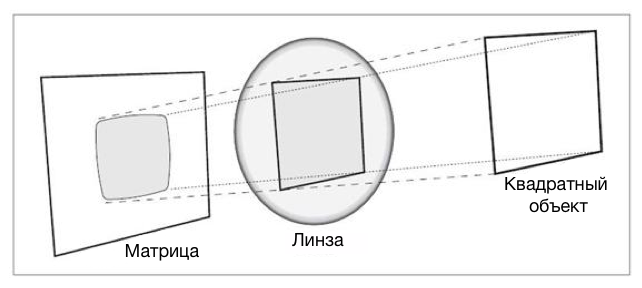
\includegraphics[width=0.8\linewidth]{pics/distorb.png}}
\caption{Искажения изображения, вносимые линзой}
\label{pic:distorb}
\end{figure}

Данный вид искажения называется радиальным. Он учитывается следующим образом:
$$
u_{corrected} = u \cdot (1 + k_1 \cdot r^2  + k_2 \cdot r^4 )
$$
$$
v_{corrected} = v \cdot (1 + k_1 \cdot r^2  + k_2 \cdot r^4 )
$$
Здесь $r$ – расстояние от точки пересечения главной оптической осью матрицы до точки проекции; $k1, k2$ – коэффициенты радиального искажения.

С учетом этих искажений формула \ref{formula:matrixProection} принимает вид:
\begin{equation}
\label{formula:matrixProection2}
q = \frac{1}{Z} \cdot \left( 
\begin{array}{ccc}
	\lambda & 0 & 0 \\ 
	0 & \lambda & 0 \\ 
	0 & 0 & 1
\end{array} 
\right) 
 \cdot M \cdot Q
\end{equation}
где $\lambda$ - корректирующая функция:
$$ \lambda = 1 + k_1 \cdot r^2  + k_2 \cdot r^4 $$

Кроме радиального искажения существует ещё тангенциальное. Оно возникает из-за того, что плоскость матрицы не перпендикулярна главной оптической оси. Но оно очень мало, и его можно не учитывать. 

При установке камеры тоже появляются погрешности – учтем их в модели.

Погрешности ориентации:
$$R_z(\theta) = 
\left( 
	\begin{array}{ccc}
	\cos (\theta ) & \sin (\theta ) & 0 \\ 
	- \sin (\theta ) & \cos (\theta ) & 0 \\ 
	0 & 0 & 1
\end{array} 
\right) 
$$

$$
R_x(\psi ) = 
\left( 
	\begin{array}{ccc}
	1  & 0 & 0 \\ 
	0 & \cos (\psi ) & \sin (\psi ) \\ 
	0 & - \sin (\psi ) & \cos (\psi ) \\ 
\end{array} 
\right) 
$$

$$
R_y(\varphi ) = 
\left( 
	\begin{array}{ccc}
	\cos (\varphi ) & 0 & - \sin ( \varphi )  \\ 
	0 & 1 & 0 \\ 
	\sin (\varphi ) & 0 & \cos (\varphi ) \\ 
\end{array} 
\right) 
$$

Результирующая матрица вращения камеры вокруг требуемой системы координат:

$$ R(\psi , \varphi , \theta ) = R_x(\psi ) \cdot R_y(\varphi ) \cdot R_z(\theta ) $$

, где $ \theta , \varphi , \psi $ - углы Эйлера.

Вектор смещения камеры относительно требуемой системы координат:
$$ 
T = 
\left( 
\begin{array}{c}
t_x \\ 
t_y \\ 
t_z
\end{array} 
\right) 
$$ 

Теперь модель камеры с учётом радиального искажения и погрешностей установки выглядит так\cite{cameraCalibrate}
$$
q = \frac{1}{Z} \cdot \left( 
\begin{array}{ccc}
	\lambda & 0 & 0 \\ 
	0 & \lambda & 0 \\ 
	0 & 0 & 1
\end{array} 
\right) 
 \cdot M \cdot R \cdot (Q + T)
$$

\subsubsection{Разработка формата и структуры данных}
В ходе функционирования подсистемы информация поступает на ее вход, получается на ее выходе, и передается между модулями внутри системы. 
При этом эта информация носит разные характер и смысл. Так как подсистема носит сугубо программный характер, то все потоки даных реализуются только программными средствами, в виде структур данных. Сетевые технологии не накладывают никаких ограничений на форматы информационных структур. 
Ниже дано описание основных форматов обмена информацией.

\begin{itemize}
\item \textbf{Видео (вход)}. Видео подается на вход системы покадрово, в связи с этим алгоритм кодирования и сжатия видео не существеннен, так как задача сформировать следующий кадр в его полном объеме ложиться на вызывающую стороную. По сути, каждый кадр представляет собой 1 картинку в формате JPEG, что проще всего представать матрицей, размер которой соответствует размеру кадра, а ее элементами являются структуры данных, хранящие информацию о каналах изображения. 

\item \textbf{Ускорения по трем осям (вход)}. Данные подаваемые с акселерометров или одного, трехосевого акселерометра. Данные имеют цифровое представления, дробное. 

\item \textbf{Угловое ускорение по трем осям (вход)}. Данные подаваемые с гироскопов или одного, трехосевого гиросокопа. Данные имеют цифровое представления, дробное. 

\item \textbf{Текущие координаты и угол поворота (выход)}. Высчитанное на текущей итерации положение объекта. Две координаты $X$ и $Y$ представляют собой целые числа. Угол поворота  $\alpha$- дробное число. Аналогиным образом можно представлять информацию о смещениях, полученных на текущей итерации. 

\item \textbf{Информационный обмен между модулем визуальной одометрии и модулем компьютерного зрения}. Данный информационых обмен происходит два раза за итерацию: для нахождения ключевых точек на кадре и для вычисления оптического потока. При этом в разных случаях содержание информационных сообщений будет разное.
	\begin{itemize}
	\item Нахождение ключевых точек - от модуля визуальной одометрии поступает изображение, являющееся кадром. Пресдставляет собой матрицу, размер которой соответствует размеру кадра, а ее элементами являются структуры данных, хранящие информацию о каналах изображения. В ответ модуль компьютерного зрения возвращает список точек в формате ${x, y}$, где $x$ и $y$ - позиция пикселя на изображении при начале отсчета в левом верхнем углу. 
	
	\item Вычисление оптического потока - от модуля визуальной одометрии поступает два изображения (текущий и предыдущий кадры)и список ключевых точек. Представление соответствует описаному ранее. В ответ модуль компьютерного зрения возвращает два списка: список смещений, представляющий собой список пар $\triangle x, \triangle y$, и вектор ошибок, состоящий из 0 и 1 - 1 означает, что соотвествующая ключевая точка не была найдена на втором изображении и вектор смещения найден ошибочно или не найден вообще. 
	
	\end{itemize}
\end{itemize}

\subsubsection{Разработка алгоритмов обработки информации}
\paragraph{Общий алгоритм работы}
\paragraph{Алгоритм вычисления оптического потока}
\paragraph{Алгоритм обработки данных с ИИУ}
\paragraph{Алгоритм сопоставления и корректировки выходных данных}



%\newpage

\section{Экономическая часть}
\subsection{Обоснование сметы  затрат на разработку программного продукта ПАОПО}

Процесс разработки сложного программного продукта сопровождается необходимостью решения многих экономических проблем. Одна из важных экономических проблем – определение стоимости программного продукта (ПП), т.е.  сметной стоимости затрат  на его разработку.

Затраты на разработку программного продукта могут быть представлены в виде сметы затрат, включающей в себя следующие статьи:
\begin{itemize}
	\item расходные материалы;
	\item затраты на оборудование;
	\item затраты на оплату труда;
	\item накладные расходы;
	\item услуги сторонних организаций;
	\item прочие расходы;
\end{itemize}

Расчет затрат на разработку данного программного продукта проводился для уровня цен и окладов на 22.04.2014г.

\subsubsection{Расчет затрат на расходные материалы}

   В статье учитываются суммарные затраты на расходные материалы, приобретаемые для разработки данного программного продукта (ПП), которые указаны в Таблице~\ref{tab:a}.
 
\renewcommand{\arraystretch}{1.4} %% increase table rowspacing   
\begin{table}[!htb]
	\caption{Стоимости расходных материалов и инструментов}\label{tab:a}
    \centering
        \begin{tabular}{|l|l|l|}
        		\hline
        		Наименование & Кол-во & Цена \\
        		\hline
        		Win Home Basic 7 SP1 32-bit Russian & 2 & 2 464 руб \\
        		\hline
        		Visual Studio Professional 2012 & 1 & 13 998 руб\\
        		\hline
        		IntelliJ IDEA 13 & 1 & 7 500 руб\\ 
        		\hline
        		IntelliJ IDEA 13 & 1 & 7 500 руб\\ 
        		\hline
        		\multicolumn{3}{|l|}{канцелярские товары}\\
        		\hline
        		писчая бумага А4 (пачка) & 1 & 140 руб\\
        		\hline
        		ручки, карандаши, ластики &   & 100 руб\\
        		\hline
        		CD – RW диск & 1 & 40 руб\\
        		\hline
        		\multicolumn{3}{|r|}{Итого: 24 242 руб }\\
        		%\hline
        		%\multicolumn{3}{|r|}{24 242 руб}\\
        		\hline
        \end{tabular}
    		
\end{table}

Получаем, что  затраты на расходные материалы составляют 
СМ=24 242 руб.


\subsubsection{Расчет затрат на оборудование}

В статье учитываются суммарные затраты на использование оборудования.
$$ 
C_{эвм}=
\frac{Ц_{эвм} \cdot Т_{эвм}}{Т_{АМР}} =
\frac{12 000 \cdot 3}{5 \cdot 12} = 
600 \; руб
$$
где, 

$C_{эвм}$ — затраты на использование (аренду) ПЭВМ для разработки программного продукта

$Ц_{эвм}$ — покупная цена вычислительной техники: $Ц_{эвм} = 12 \; 000 \; руб$

$Т_{эвм}$ — время использования ПЭВМ для разработки данного программного продукта в месяцах (3 месяца)

$Т_{АМР}$ – срок амортизации вычислительной техники, составляет 5 лет. 

Тогда $Т_{АМР} = 5 \; лет =5 \cdot 12 = 60 \; месяцев $.

Затраты на ремонт вычислительной техники составляют 5\% от  стоимости ее использования и равны:
$$C_{рем} = 0,05 \cdot C_{эвм} = 30 \; руб$$

Получаем, что  затраты на оборудование с учетом его ремонта составляют:
$ С_{ОБ} = С_{ЭВМ} + С_{РЕМ} =  600 + 30 = 630 \; руб$.

\subsection{Определение трудоемкости выполнения проекта}
Трудоемкость разработки проекта по каждому участнику может быть определена как сумма величин трудоемкости выполнения участниками отдельных стадий.

В соответствии с ГОСТ 19.102-94 “Стадии разработки” процесс разработки ПОАПО разбивается на пять стадий: разработка ТЗ, эскизное проектирование, техническое проектирование, рабочее проектирование и внедрение. Этот ГОСТ допускает в технико-обоснованных случаях исключать стадии эскизного и технического проектов, то есть объединять техническое и рабочее проектирование. Трудоемкость каждого этапа указывается в часах и приведена в  Таблице~\ref{tab:b}.

\begin{table}[!htb]
	\caption{Трудоемкость по этапам проектирования}\label{tab:b}
    \centering
        \begin{tabular}{|p{4cm}|p{5.5cm}|l|l|}
        		\hline
        		\multirow{2}{4cm}{Стадия} & \multirow{2}{*}{Этап} & \multicolumn{2}{c|}{Трудоёмкость (часы)} \\
        		\cline{3-4}
            	& & Аналитик & Разработчик \\
            	\hline	
            	\multirow{3}{*}{1. Разработка ТЗ} 
            						& 1.1 Формулировка и уточнение задания. 
            						& 20 & – \\
            	\cline{2-4}	
                					& 1.2. Исследование и анализ ПО. 
            						& 80 & – \\
            	\cline{2-4}	
            	    					& 1.3. Разработка и утверждение ТЗ. 
            						& 40 & – \\
            	\hline	
            	\multirow{3}{4cm}{2. Рабочее
проектирование
} 
            						& 2.1. Техническое проектирование (разработка моделей данных и алгоритмов).
            						& 200 & 20 \\
            	\cline{2-4}	
                					& 2.2. Рабочее проектирование (кодирование и тестирование программных модулей). 
            						& 20 & 160 \\
            	\cline{2-4}	
            	    					& 2.3. Тестовые испытания системы. 
            						& 20 & 100 \\
            	\cline{2-4}	
            	    					& 2.4. Разработка программной документации.
            						& 60 & - \\						
        		\hline
        		3. Внедрение & 3.1. Подготовка проекта к внедрению. & 40 & 20 \\
        		\hline
        		\multicolumn{2}{|l|}{Итого по участникам:} & 480 & 300 \\
        		\hline
        		\multicolumn{2}{|l|}{Итого:} & \multicolumn{2}{c|}{ 780 } \\
        		\hline
        \end{tabular}   		
\end{table}

Для определения трудоемкости разработки проекта по каждому участнику в человеко-днях, используем следующую формулу: 
$$ T_{рд} = Т_{час}/t_{рд},$$
где $Т_{час}$ – время на разработку в часах, $t_{рд}$ – коэффициент, показывающий количество рабочих часов в одном дне. Для дальнейших расчетов примем $t_{рд} = 8\; час$

Для аналитика $T_{рд} = Т_{час}/t_{рд} = 480/8 = 60 \; дней$.

Для разработчика $T_{рд} = Т_{час}/t_{рд} = 300/8 = 38 \; дней$.

Или, суммарно, – 98 рабочих дней.

Для определения времени реализации проекта требуется перевести рабочие дни в календарные дни (КД). Для перевода используется следующая формула:

$$Т_{кд}=\frac{T_{РД} \cdot (1+d) }{g},$$
где $d$ – доля дополнительных работ, порученных другой группе работников попутно с основной работой (от 0,1 до 0,3). В нашем случае проект ведётся самостоятельно, $d = 0$, $g$ – коэффициент перевода (в зависимости от выходных и праздничных дней) – 0,73.

Дня аналитика: $Т_{кд}={T_{РД} \cdot (1+d) }/{g} = 60/0,73 = 83 $ календарных дня.

Для разработчика: $Т_{кд}={T_{РД} \cdot (1+d) }/{g} = 38/0,73 = 52 $ календарных дня.

Или, суммарно, – 135 календарных дней.

\subsection{Расчет затрат на оплату труда}

В данную статью включается заработная плата исполнителей, непосредственно связанных с разработкой программного продукта, с учетом их должностного оклада и времени участия в разработке. 

Основная заработная плата рассчитывается по формуле:
$$ЗП_{осн}=T_{д} \cdot L_{ср.дн.},$$
где $T_{д}$ – трудоемкость, календарные дни, $L_{ср.дн.}$ – среднедневной заработок работника. 

Для определения средней заработной платы аналитика-руководителя небольшого проекта и программиста-разработчика проведен анализ основных ресурсов, предоставляющих сервисы для поиска работы и дающих возможность оценить размер компенсации труда. Такой подход позволяет оценить максимально приближенную к реальности рыночную стоимость труда.

Использованные ресурсы:
\begin{itemize}
	\item портал поиска предложений по трудоустройству HeadHunter. Адрес: www.hh.ru
	\item портал поиска предложений по трудоустройству Job.ru. Адрес: www.job.ru.
\end{itemize}

В результате в качестве средней заработной платы аналитика-руководителя проекта было взято 50 тыс. руб., программиста – 60 тыс. руб.

Тогда среднедневной заработок находится по формуле:

$$L_{ср.дн.}=L_{0}/F,$$ 
где $L_{0}$ – среднемесячная заработная плата, $F$ – среднее количество рабочих дней в месяце. F вычисляется по следующей формуле:

$$ F = \frac{\sum N_{раб}}{n} = \frac{18+19+22}{3} = 19,$$
где $N_{раб}$ – количество рабочих дней в месяце, $n$ – число месяцев.

В данном случае n = 3.

Тогда, для аналитика $L_{ср.дн.}= 50 000 / 19 = 2 631 руб.$ и расходы на основную зарплату составят: $ЗП_{осн} = 2 631 \cdot 60 дней \approx 158 000 руб.$

Тогда, для разработчика  $ L_{ср.дн.}= 60 000 / 19 = 3 157 руб.$ и расходы на основную зарплату составят: $ЗП_{осн} = 3 157 \cdot 38 дней \approx 120 000 руб.$

\textbf{Дополнительная  заработная плата.}

Расходы на дополнительную заработанную плату учитывают все выплаты непосредственно исполнителям за время не проработанное на производстве, но предусмотренное законодательством, в том числе: оплата очередных отпусков, компенсация за недоиспользованный отпуск, и др. Величина этих выплат составляет 20\% от размера основной заработной платы:

$$С_{зпд} = 0,2 \cdot С_{зпо} = 0,2 \cdot 278\;000 = 55\;600 \; руб$$

В результате получаем, что  затраты на  оплату труда составляют:
$$С_{зпи} = С_{зпо} + С_{зпд} = 278\;000 + 55\;600 = 333\;600 руб.$$

\subsubsection{Расчет затрат на  страховые взносы}

В данной статье затрат учитываются отчисления на социальные нужды, производимые в фонды социального страхования, обязательного медицинского страхования и пенсионный фонд. Расчет производится с учетом законов, принятых с 1 января 2012 года (отдельные положения вступают в иные сроки):

Федеральный закон от 24.07.2009  \textnumero 212 ФЗ (ред. от 28.12.2013) <<О страховых взносах в Пенсионный фонд Российской Федерации, Фонд социального страхования Российской Федерации, Федеральный фонд обязательного медицинского страхования и территориальные фонды обязательного медицинского страхования>>;

Федеральный закон от 24.07.2009 \textnumero 213 ФЗ (ред. от 07.05.2013) <<О внесении изменений в отдельные законодательные акты Российской Федерации и признании утратившими силу отдельных законодательных актов (положений законодательных актов) Российской Федерации в связи с принятием Федерального закона <<О страховых взносах в Пенсионный фонд Российской Федерации, Фонд социального страхования Российской Федерации, Федеральный фонд обязательного медицинского страхования и территориальные фонды обязательного медицинского страхования>>.

С 1-го января 2006 года согласно федеральному закону РФ \textnumero 158-ФЗ от 6.12.2005 года величина единого социального налога рассчитывается по формуле:

$$ С_{сн}=К^{сн} \cdot C_{зп},$$
где $К^{сн}$ – коэффициент, учитывающий социальный налог, $C_{зп}$ – заработная плата (руб.)

Плательщиками страховых взносов являются страхователи, определяемые в соответствии с федеральными законами о конкретных видах обязательного социального страхования, к которым относятся:
\begin{enumerate}
\item лица, производящие выплаты и иные вознаграждения физическим лицам: 
\begin{itemize}
\item организации;
\item индивидуальные предприниматели;
\item физические лица, не признаваемые индивидуальными предпринимателями;
\end{itemize}
\item индивидуальные предприниматели, адвокаты, нотариусы, занимающиеся частной практикой, и иные лица, занимающиеся в установленном законодательством Российской Федерации порядке частной практикой (далее - плательщики страховых взносов, не производящие выплаты и иные вознаграждения физическим лицам), если в федеральном законе о конкретном виде обязательного социального страхования не предусмотрено иное.
(в ред. Федерального закона от 03.12.2011 \textnumero 379-ФЗ).
Для страхователей, перечисленных выше, предусмотрены следующие ставки:
\end{enumerate}
\begin{table}[!htb]
    \centering
        \begin{tabular}{|l|l|l|}
        		\hline
        		ПФР & ФСС & ФФОМС \\
        		\hline
        		22\% & 2,9\% & 5,1\% \\
        		\hline
        \end{tabular}   		
\end{table}

Отсюда  $К^{сн} = 0,3$  и таким образом затраты на единый социальный налог составляют: $С_{СН} = 0,3  \cdot 333 \; 600  \; руб = 100 \; 080 \; руб.$

\subsubsection{Расчет затрат на услуги сторонних организаций} 

В статье учитываются затраты на выполнение сторонними организациями работ, непосредственно связанных с разработкой программного продукта.

При разработке данного продукта потребовались услуги сторонних организаций по изготовлению 10-ти плакатов формата A1 и печати на принтере 300 листов РПЗ формата А4.  Стоимость распечатки плакатов  (СПЛ) и листов РПЗ (СЛ) соответственно  рассчитываются  по формулам:
$$С_{ПЛ} =10 \cdot С_{А1} = 10 \cdot 150 = 1500 \; руб,$$
где $С_{А1}$ – стоимость распечатки одного плаката формата A1.   $С_{А1}  = 150 руб.$.
$$С_Л =300 \cdot С_{А4} = 300 \cdot 2 = 600 \; руб.,$$
где $С_{А4}$ – стоимость распечатки одного листа  формата А4. $С_{А4}  = 2 \; руб.$

Получаем, что затраты на услуги сторонних организаций составляют
$С_{ИЗГ}= С_{ПЛ} + С_Л = 2100 \; руб.$

\subsubsection{Расчет затрат на накладные расходы}
В данной статье учитываются затраты на общехозяйственные расходы (это плата за здание, в котором идет разработка, его ремонт, плата за энергоресурсы), непроизводственные расходы и расходы на управление.
Накладные расходы составляют 12,5\% + 25\% требуемого уровня рентабельности.
 
$С_{НР}  =(0,125+0,25) \cdot (С_М + С_{ОБ} + С_{ЗП} + С_{СН} + С_{ИЗГ})$

Таким образом,  затраты на накладные расходы составляют:  
$С_{НР}  = (0,125+0,25) \cdot (18 \; 480+ 630 + 333 \; 600+ 100 \; 080 + 2 \; 100) =170 \; 583,75 руб.$

\subsubsection{Расчет прочих расходов}

Данная статья расходов учитывает налог на имущество и налог на транспортные средства. Налог на имущество в данном случае не платится, так как  все имущество, включаемое в налогооблагаемую базу в соответствии с инструкцией «О порядке исчисления и уплаты в бюджет налога на имущество предприятий», используется на нужды образования, и, следовательно, налогом на имущество не облагается.

Налог на владельцев транспортных средств не платится, в связи с отсутствием транспортных средств. 

\subsubsection{Итог затрат для заказчика}

Итог затрат для заказчика рассчитывается как сумма по всем вышеперечисленным статьям затрат и составляет:

$Ц = 24 \; 242+ 630 + 333 \; 600  + 100 \; 080  + 2100 + 170 \; 583   =  625 \; 473  руб.$

Смета затрат на разработку программного продукта приведена в Таблице~\ref{tab:c}.

\begin{table}[!htb]
	\caption{Стоимости расходных материалов и инструментов}\label{tab:c}
    \centering
        \begin{tabular}{|l|l|l|}
        		\hline
        		\textnumero п/п & Статья затрат & Сумма статьи (руб.) \\
        		\hline
        		1 & Расходные материалы & 24 242 \\
        		\hline
        		2  & Затраты на оборудование & 630 \\
        		\hline
        		3  & Затраты на оплату труда & 333 600 \\
        		\hline
        		4  & Услуги сторонних организаций & 2 100 \\
        		\hline
        		5  &  Накладные расходы & 170 583 \\
        		\hline
        		6 & Прочие расходы & - \\
        		\hline
        		7 & Цена & 631 315 \\
        		\hline
        \end{tabular}   		
\end{table}


\subsection{Основные сметы затрат на тестирование, внедрение и эксплуатацию системы}

Далее рассчитаем затраты на внедрение и эксплуатацию программного продукта ПАОПО.

\subsubsection{Тестирование}
Для тестирования разрабатываемой подсистемы необходимо выполнить следующие пункты:
\begin{itemize}
\item сопрячь ПАОПО с видеокамерой;
\item сопрячь ПАОПО с инерциальными измерительными приборами;
\item провести тестирование ПАОПО, фиксируя перемещения с помощью GPS-трекера;
\item наложить полученные с помощью ПАОПО данных на данные, полученные с помощью GPS-трекера.
\end{itemize}

Таким образом необходимо закупить следующее оборудование:
\begin{itemize}
\item видеокамера с разрешением 720*1080;
\item трехосевой гироскоп;
\item трехосевой акселерометр;
\item GPS-трекер;
\end{itemize}

Данное оборудование установлено во всех современных смартфонах, работающих под управлением ОС Android, стоимость которых в настоящее время составляет 6 000 рублей и более. Например, телефон HTC Sensation, удовлетворяющий всем требованиям стоит 6200 рублей. 

Для проведения сопряжения полученных данных с ПАОПО необходимо написать простое приложение, фиксирующее все данные в нужном формате для анализа разрабатываемой подсистемы, разработка которого займет до двух рабочих дней Android-разработчка. 

Согласно приведенным выше данным стоимость одного дня разработчика составляет 3 157 рублей. С учетом дополнительных расходов и отчислений в страховые фонды затраты на создание приложения составят:

$$31571,2 \cdot 1,3 \cdot 2=9 \; 849 \; руб$$

Таким образом затраты на тестирование составят 16 149 рублей.

\subsubsection{Внедрение и эксплуатация}

В рамках создания ПАОПО не предусмотрены внедрение и эксплуатация, так как подсистема может работать лишь в составе другой автономной системы. 

ПАОПО является кроссплатформенной, что позволяет в кратчайшие сроки интегрировать ее в любую другую систему. При этом разработчику этой системы необходимо согласовать вход и выход ПАОПО, корректно предоставляя и получая данные в/из подсистемы. Суммарные затраты на проведение интеграции могут занимать до двух рабочих дней разработчика. Согласно приведенным выше данным стоимость этой работы составит не более 6 314 рублей. 

Однако данные затраты не относятся к стоимости создания ПАОПО, а перекладываются на ее потребителей. 

\subsection{Итого. Расходы на разработку  и тестирование.}
\begin{table}[tb!h]
	\caption{Итого. Расходы на внедрение и эксплуатацию системы.}
    \centering
        \begin{tabular}{|l|l|l|}
        		\hline
        		\textnumero п/п & Статья затрат & Сумма статьи (руб.) \\
        		\hline
        		1 & Стоимость программного продукта ПОАПО & 631 315 \\
        		\hline
        		\multicolumn{3}{|r|}{\textbf{Итого: 647 646} }\\
        		\hline
        \end{tabular}   		
\end{table}                        %
%\newpage

\section{Техническое задание}

Исходные данные представлены в таблице~\ref{table:ishodn_dann}.

\begin{table}[ht]
\caption{Исходные данные, 19 вариант}
\label{table:ishodn_dann}
\centering
 \begin{tabular}{|c|c|c|c|c|c|c|}
 \hline Офис & 1 ф & 2 ф & ОС, СУБД и оборудование & ЦП & Диски & Модель \\
 \hline 6(2)/2(2) & 3(4)/2(4) & 14 & 24/34/44 & 54 & 64(3)(0.6) & 74 \\
 \hline
 \end{tabular}
\end{table}

\subsection{Наименование}

Проектирование распределённой АСОИиУ фирмы.

\subsection{Основание для разработки}

Основанием для разработки является учебный план кафедры ИУ5 МГТУ им. Н.Э. Баумана. 

\subsection{Цель разработки}

Целью разработки является создание проектного решения на распределенную сеть обработки информации, объединяющую все подразделения фирмы, состоящей из центрального и двух удаленных офисов.

\subsection{Задачи, подлежащие решению}

В процессе выполнения курсовой работы необходимо решить следующие задачи:
\begin{enumerate}
\item Разработать блок-схему распределенной АСОИиУ фирмы и структурные схемы ЛВС центрального и удаленных офисов фирмы;
\item Описать правила построения всех сетей фирмы;
\item Выбрать и обосновать вариант удаленной связи отдельных ЛВС фирмы;
\item Выбрать требуемое оборудование для ЛВС фирмы;
\item Описать настройку рабочих параметров сетевой ОС, под управлением которой работают ЛВС фирмы;
\item Описать настройку рабочих параметров СУБД, которая установлена в ЛВС фирмы;
\item Провести распределение предметных баз данных по узлам сети;
\item Выполнить аналитическое и имитационное моделирование ЛВС фирмы и провести сравнительный анализ результатов моделирования;
\item Разработать и представить рекомендации по модернизации и реорганизации распределенной АСОИиУ фирмы.
\end{enumerate}

\subsection{Требования к составу технических средств}

Фирма состоит из центрального офиса и двух удалённых филиалов.\par\bigskip

В центральном офисе фирмы расположены ЛВС 100BASE-T4, содержащая 2 концентратора, и ЛВС 10BASE-2, содержащая 2 сегмента. Обе сети подключены к коммутатору, к которому также подключён удаленный маршрутизатор с двумя модемами.\par\bigskip

В первом филиале фирмы расположены ЛВС 10BASE-T, содержащая 4 концентратора, и ЛВС 10BASE-2, содержащая 4 сегмента. Обе сети подключены к коммутатору, к нему также подключен удаленный маршрутизатор с одним модемом.\par\bigskip

Во втором филиале фирмы расположена ЛВС Token Ring на STP c усилителями.\par\bigskip

В сети установлен сервер на базе 4 ядерного процессора с дисковой подсистемой уровня RAID-6.
 
\subsection{Требования к составу программных средств}

ЛВС работают под управлением сетевой ОС Windows 7. В сети установлена СУБД Sybase.

\subsection{Техническая документация, предъявляемая по окончании работы}

По окончании работы должна быть предъявлена следующая документация:
\begin{itemize}
\item структурная схема объединённой сети фирмы;
\item распределение предметных баз данных по узлам сети;
\item формализованная схема сети и результаты моделирования;
\item пояснительная записка.
\end{itemize}

\subsection{Порядок приема работы}

Приём работы осуществляется путем проверки соответствия выполненной работы пунктам технического задания.

\subsection{Дополнительные условия}

Определить вероятность безотказной работы дисковой подсистемы сервера, построенной на базе RAID-6, содержащей 3 базовых диска (без учета уровня RAID), при условии, что вероятность безотказной работы одного диска равна 0.6 и все диски одинаковые.\par\bigskip
 
Необходимо провести сравнительный анализ серверов отдела на базе 4 ядерных процессоров и выбрать наилучший. Подробно описать особенности эксплуатации блока питания и ИБП.\par\bigskip

Модель системы должна соответствовать общему виду, чтобы можно было провести исследование любого варианта. Результаты моделирования должны соответствовать варианту задания, по-этому необходимо провести моделирование системы, содержащей 19 рабочих станций и сервер (ЦП и диски).                             % Техническое задание
%\newpage

\section{Архитектура объединённой сети фирмы}

\subsection{Общая схема сети}

Объединенная сеть состоит из сети центрального офиса, сети 1 филиала и сети 2 филиала. Её общая схема изображена на рисунке~\ref{pic:3_1}. В графических обозначениях схема изображена на рисунке~\ref{pic:3_2}.

\begin{figure}[h]
\center{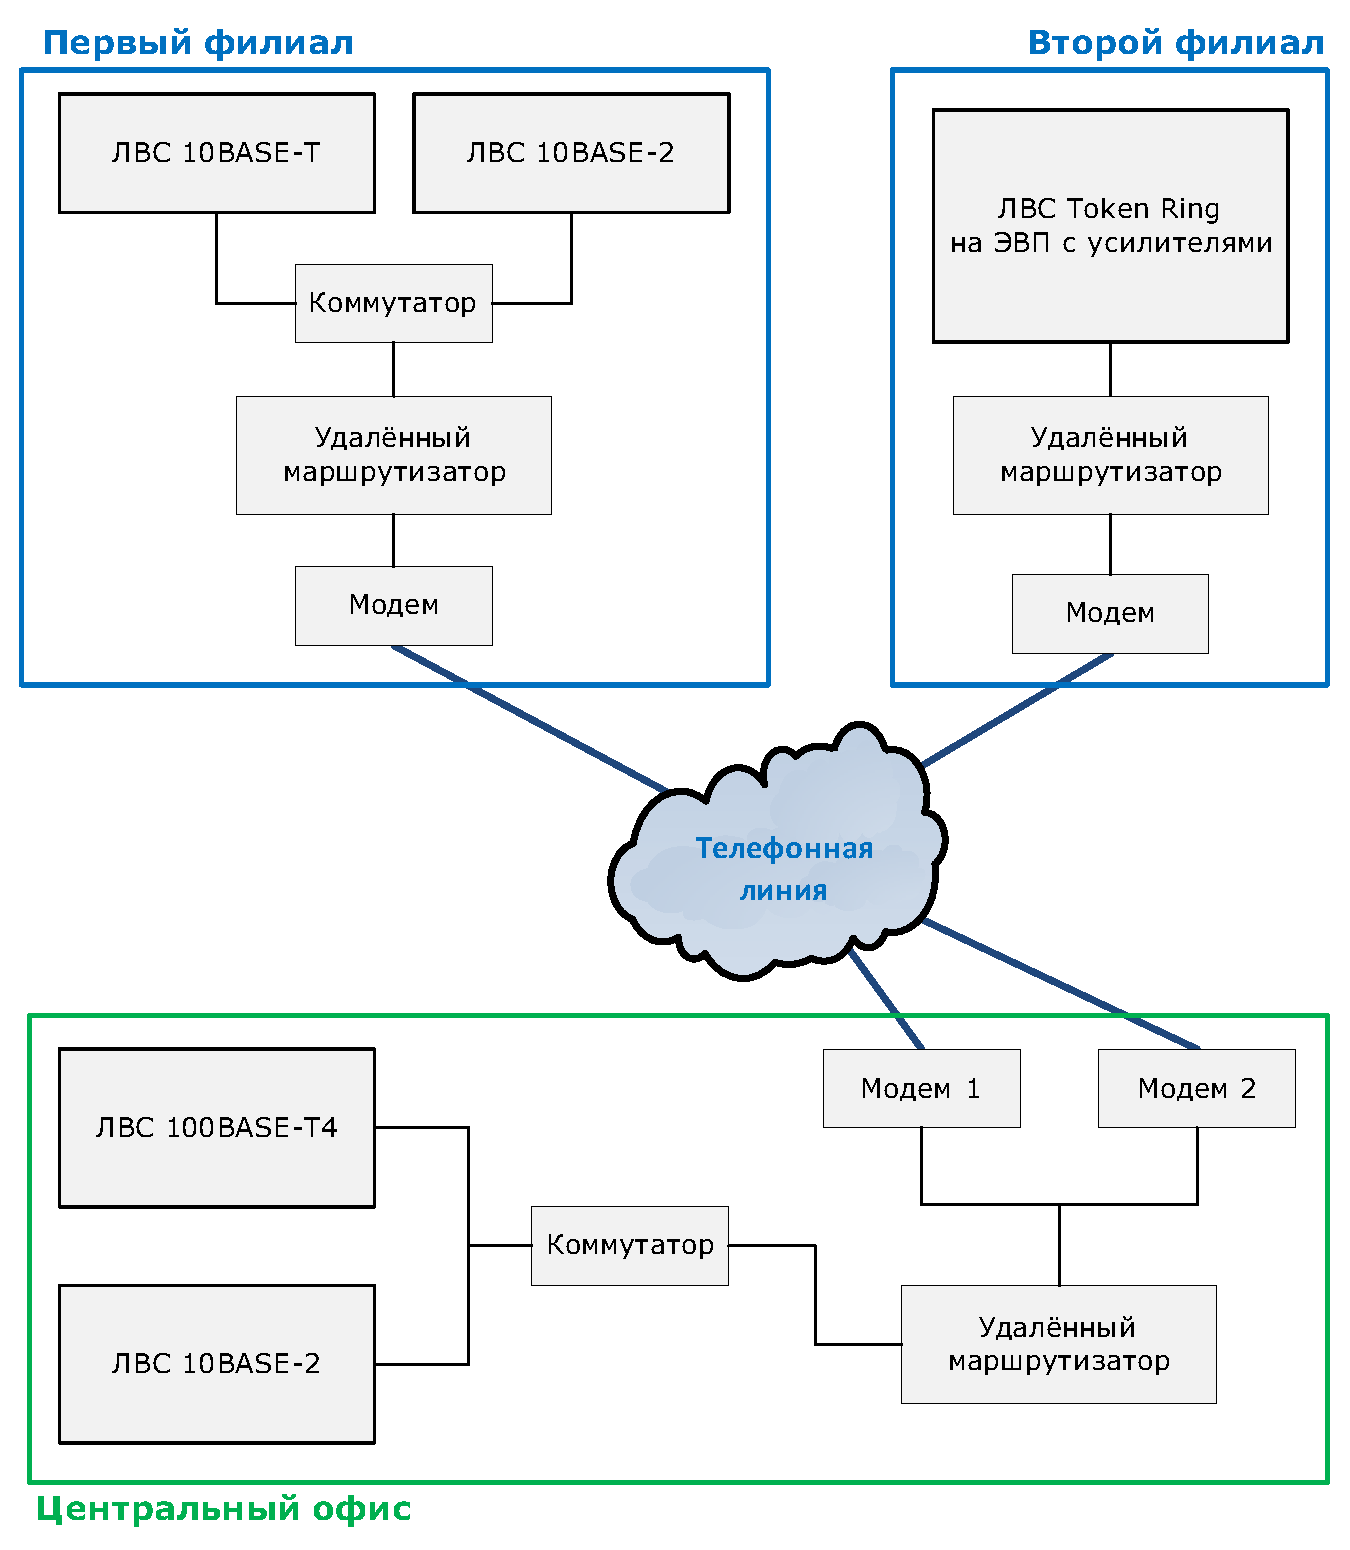
\includegraphics[width=0.6\linewidth]{pics/pic3_1.eps}}
\caption{Общая схема РСОД фирмы.}
\label{pic:3_1}
\end{figure}

В центральном офисе фирмы расположены ЛВС 100BASE-T4 и ЛВС 10BASE-2. Обе сети подключены к коммутатору, к которому также подключён удаленный маршрутизатор с двумя модемами.\par\bigskip

В первом филиале фирмы расположены ЛВС 10BASE-T и ЛВС 10BASE-2. Обе сети подключены к коммутатору, к нему также подключен удаленный маршрутизатор с одним модемом.\par\bigskip

\newpage

Во втором филиале фирмы расположена ЛВС Token Ring на STP c усилителями.

\begin{figure}[h]
\center{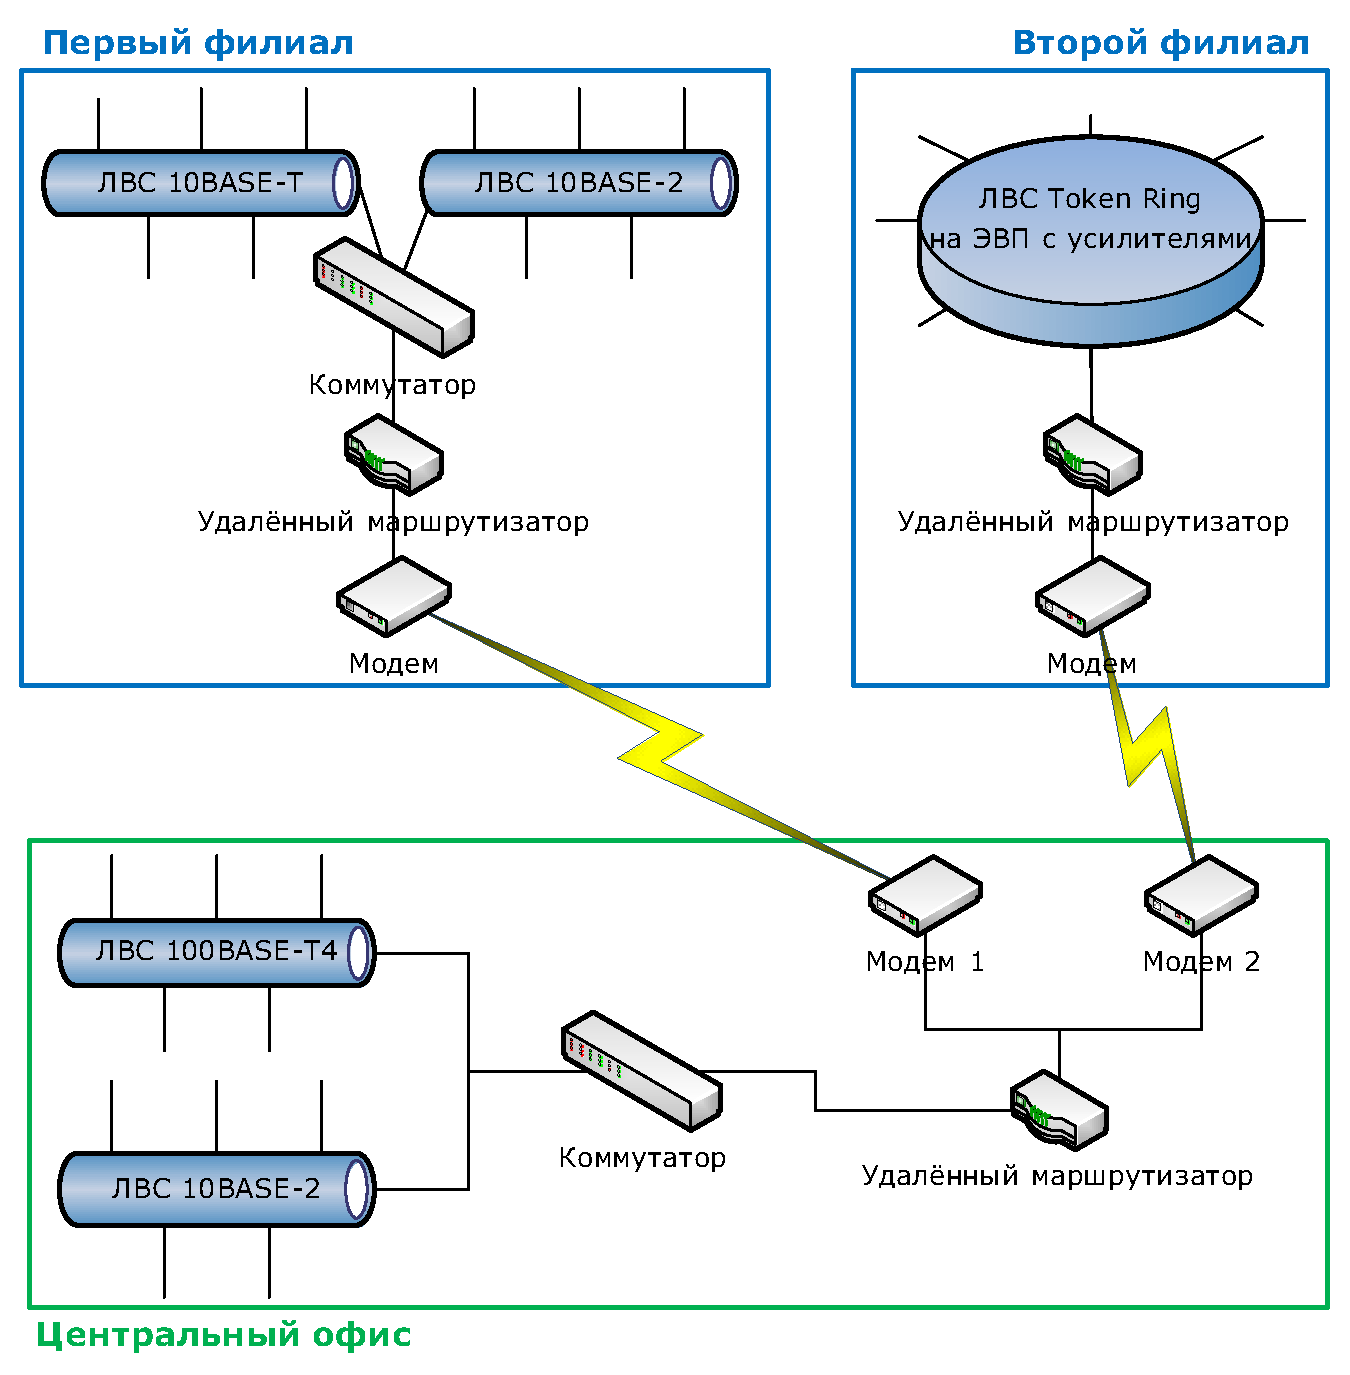
\includegraphics[width=0.6\linewidth]{pics/pic3_2.eps}}
\caption{Общая схема РСОД фирмы в графических обозначениях.}
\label{pic:3_2}
\end{figure}

\newpage

\subsection{Схема сети центрального офиса}

В центральном офисе фирмы расположены ЛВС 100BASE-T4, содержащая 2 концентратора, и ЛВС 10BASE-2, содержащая 2 сегмента. Обе сети подключены к коммутатору, к которому также подключён удаленный маршрутизатор с двумя модемами. В офисе также находится сервер фирмы. Схема сети представлена на рисунке~\ref{pic:3_3}.

\begin{figure}[h]
\center{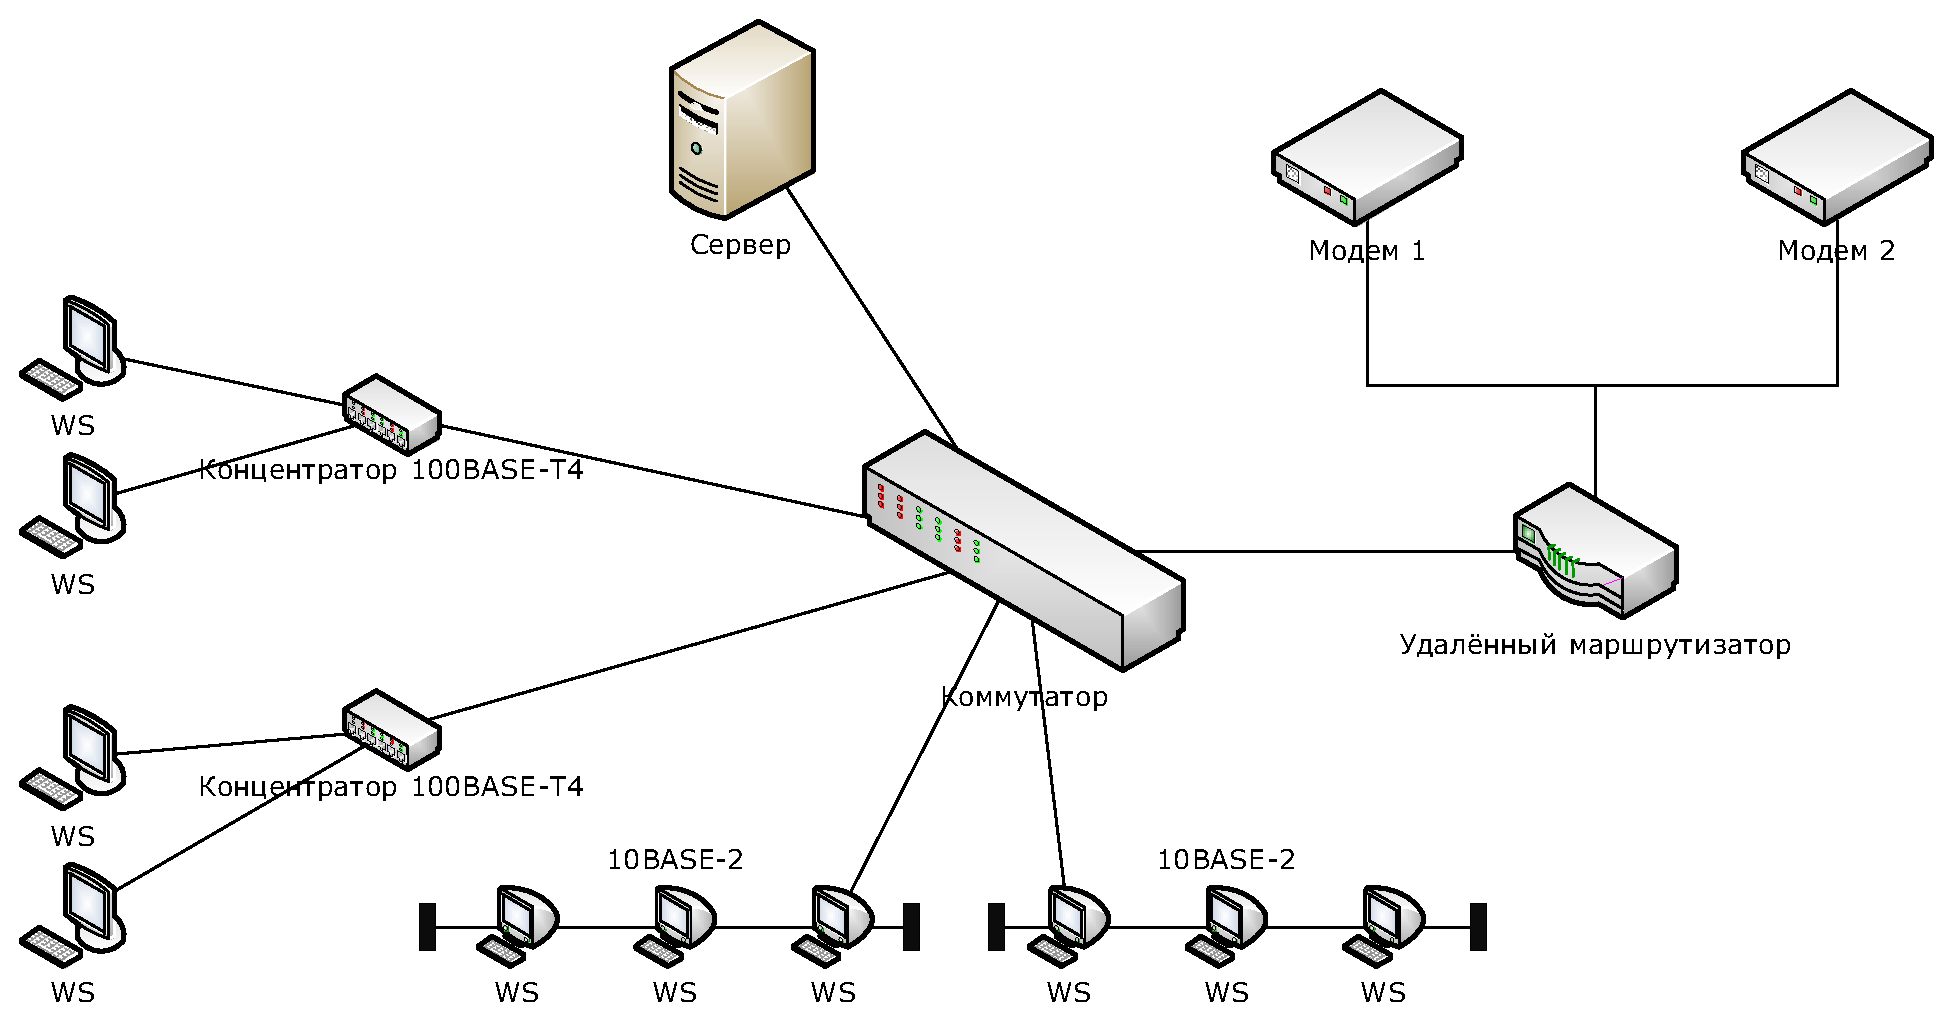
\includegraphics[width=0.6\linewidth]{pics/pic3_3.eps}}
\caption{Схема сети центрального офиса.}
\label{pic:3_3}
\end{figure}

\newpage

\subsection{Схема сети первого филиала}

В первом филиале фирмы расположены ЛВС 10BASE-T, содержащая 4 концентратора, и ЛВС 10BASE-2, содержащая 4 сегмента. Обе сети подключены к коммутатору, к нему также подключен удаленный маршрутизатор с одним модемом. Схема сети представлена на рисунке~\ref{pic:3_4}.

\begin{figure}[h]
\center{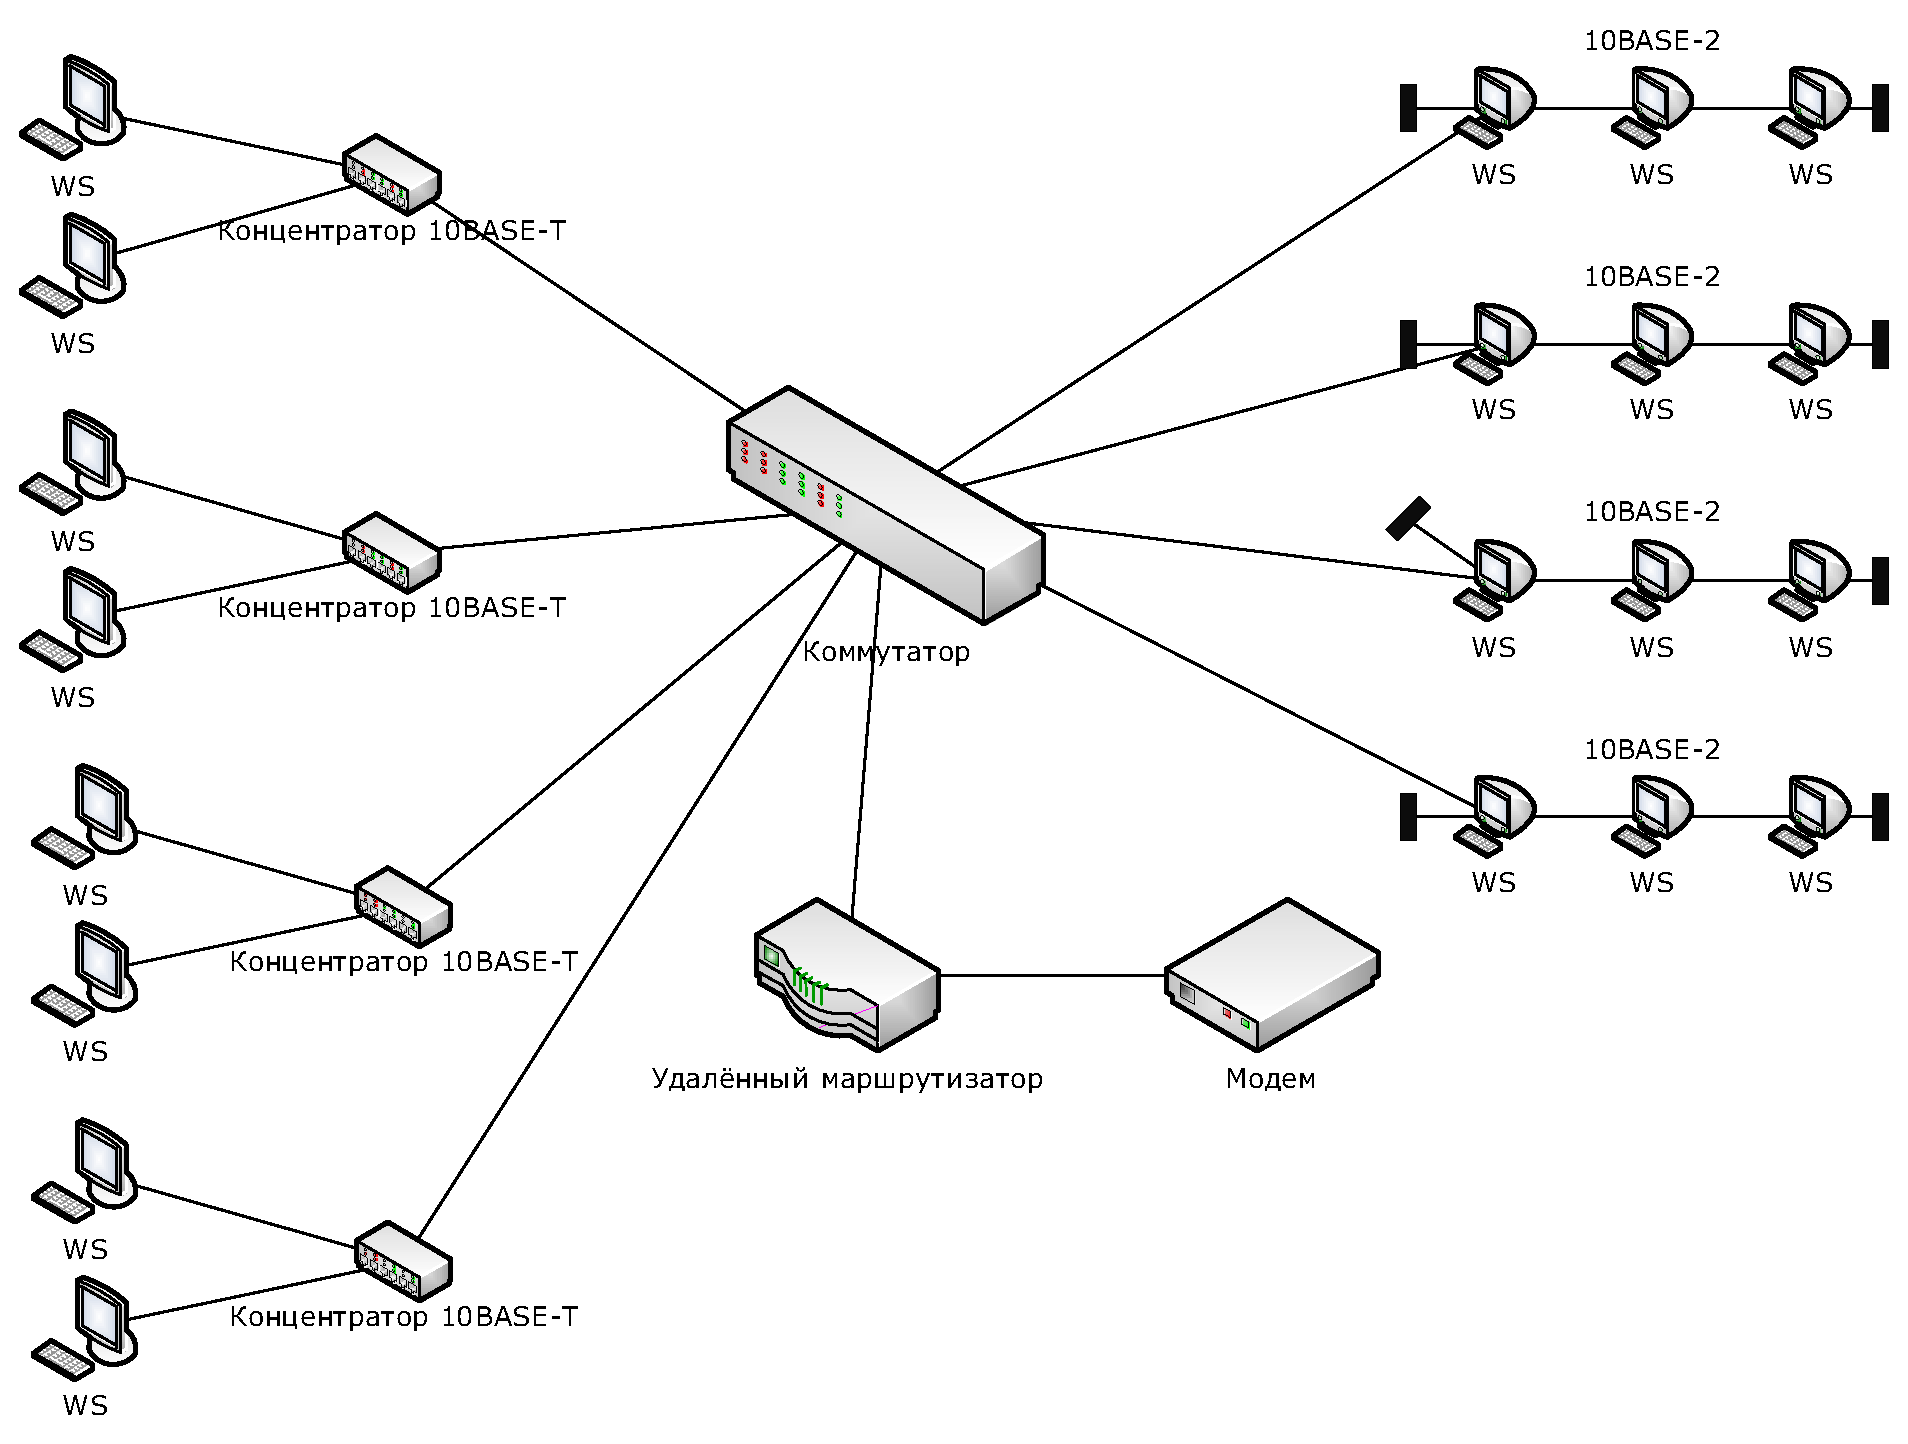
\includegraphics[width=0.6\linewidth]{pics/pic3_4.eps}}
\caption{Схема сети первого филиала.}
\label{pic:3_4}
\end{figure}

\newpage

\subsection{Схема сети второго филиала}

Во втором филиале фирмы расположена ЛВС Token Ring на STP с усилителями. Схема сети представлена на рисунке~\ref{pic:3_5}.

\begin{figure}[h]
\center{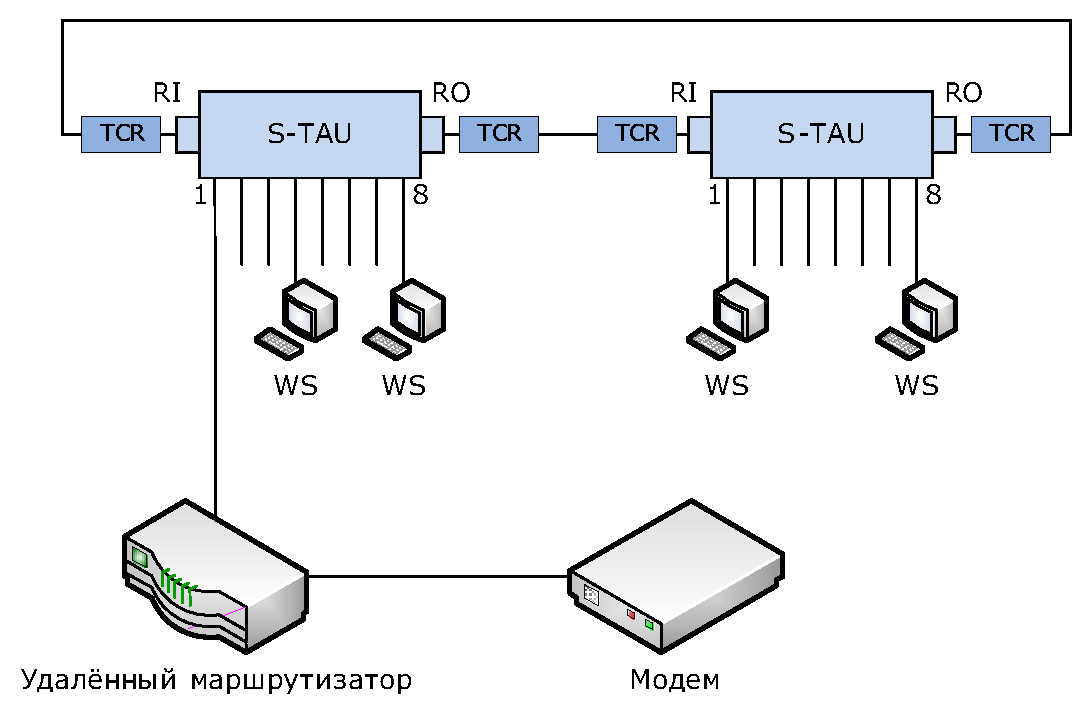
\includegraphics[width=0.6\linewidth]{pics/pic3_5.eps}}
\caption{Схема сети второго филиала.}
\label{pic:3_5}
\end{figure}

\newpage

\subsection{Правила построения сети}

Для построения работоспособной сети следует придерживаться ряда правил.

\subsubsection{Правила построения сетей 100BASE-T4}

При построении сети на основе 100BASE-T4 применяются следующие правила:
\begin{itemize}
\item для перехода с технологии TX на T4 требуется заменить концентраторы и сетевые адаптеры, тогда не придётся менять километры кабеля, так как кабель используется тот же;
\item в кабеле используются все 4 пары;
\item длина луча сети должна быть не более 100 метров;
\item между любыми двумя узлами сети расстояние должно быть не более 205 м;
\item между любыми двумя узлами должно быть не более 5 сегментов и 4 повторителей;
\end{itemize}

\subsubsection{Правила построения сетей 10BASE-2}

При построении сети на основе 10Base2 применяются следующие правила:
\begin{itemize}
\item используется тонкий коаксиальный кабель с терминаторами на обоих концах;
\item для усиления сигнала используются повторители;
\item повторители должны быть подключены к источнику электропитания;
\item рабочие станции подключаются к кабелю с помощью сетевых адаптеров с разъёмом BNC и T-коннекторов;
\item один из терминаторов каждого сегмента заземляется;
\item T-коннектор подключается к терминатору непосредственно или через расстояние кратное 2.5 м;
\item минимальное расстояние между двумя Т-коннекторами составляет 2.5 м;
\item расстояние между двумя Т-коннекторами должно быть кратно 2.5 м;
\item между любыми двумя узлами должно находиться не более 5 сегментов, 4 повторителей;
\item длина сегмента не более 185 м;
\item длина сети не более 925 м;
\item к сегменту может быть подключено не более 30 узлов.
\end{itemize}

\subsubsection{Правила построения сетей 10BASE-T}

При построении сети на основе 10Base2 применяются следующие правила:
\begin{itemize}
\item длина сегмента – 100 метров;
\item между двумя узлами может быть не выше 5 лучей; 
\item общее количество станций не должно превышать 1024;
\item максимальное число концентраторов между любыми двумя станциями сети - 4;
\item мксимальный диаметр сети - 500 м;
\item используются коннекторы RJ-45;
\item не допускается образование колец;
\item используется неэкранированная витая пара 3 категории.
\end{itemize}

\subsubsection{Правила построения сетей Token Ring}

При построении сети на основе Token Ring STP применяются следующие правила:
\begin{itemize}
\item в качестве кабеля используется экранированная витая пара (STP);
\item для доступа с сети используются S-TAU (не более 12 штук);
\item максимум в сети может быть 255 узлов;
\item применяются усилители на медном кабеле (TCR), расстояние между устройствами доступа составляет 300 м;
\item максимальная длина луча без усилителя составляет 100 м.
\end{itemize}
                           % Архитектура сети
%\newpage

\section{Построение сети}

\subsection{Принципы построения производительных сетей}

Производительность системы определяется сочетанием её аппаратно- программных средств. Повышение производительности может быть достигнуто путем использования аппаратных средств, обладающих лучшими характеристиками производительности по сравнению с уже применяющимися.\par\bigskip

Повышение производительности сервера, следует производить в соответствии с предварительными расчетами “узких мест” – аналитическими расчетами, либо с помощью моделирования его работы. Эти расчеты показывают целесообразность увеличения производительности того или иного узла сервера - процессора, дисковой подсистемы. Аналогично для ЛВС можно определить, например, актуальность увеличения пропускной способности каналов связи.\par\bigskip

Производительность сервера зависит от наличия: 
\begin{itemize}
\item количества центральных процессоров;
\item шин PCI и их большой производительности;
\item большого объема памяти ОЗУ;
\item высокоскоростного дискового интерфейса;
\item организация дисковых подсистем с использованием RAID, обеспечивающих увеличение производительности.
\end{itemize}

\subsection{Принципы построения отказоустойчивых сетей}

Отказоустойчивость сети определяется двумя факторами:
\begin{itemize}
\item уровень избыточности сетевой инфраструктуры;
\item время восстановления сети, то есть время, необходимое для переключения потоков данных на работоспособные части сети в случае отказа ее части.
\end{itemize}\par\bigskip

При построении отказоустойчивой системы необходимо учесть следующее:
\begin{enumerate}
\item Архитектура сетевого оборудования:
    \begin{itemize}
    \item дублирование блоков питания;
    \item возможность "горячей" замены компонентов; 
    \item дублирование управляющего модуля; 
    \item ублирование коммутационной матрицы/шины.
    \end{itemize}
\item Дублирование соединений:
    \begin{itemize}
    \item использование нескольких дублирующих соединений; 
    \item не рекомендуется использовать протокол Spanning Tree, так как в сети появляется много неработающих (заблокированных) соединений, а время восстановления очень большое; 
    \item желательно использовать технологии Multi-Link Trunk (MLT) и Split-MLT (автоматическая балансировка потоков данных между всеми работоспособными соединениями; восстановление сети за доли секунды); 
    \item возможно внедрение протоколов балансировки нагрузки и дублирования на уровне маршрутизации;
    \item разнесение окончания каналов - окончание каналов на разных модулях ввода/вывода и/или на разных узлах для дополнительного дублирования;
    \item разнесение каналов - использование различных носителей и различных путей для критичных соединений;
    \end{itemize}
\item Высоконадежное сетевое оборудование - устройства с высоким временем наработки на отказ;
\item Отказоустойчивость сервера:
    \begin{itemize}
    \item использование технологии PCI Hot Plug замены отдельных узлов;
    \item многопроцессорные серверы;
    \item организация дисковых подсистем с использованием RAID, обеспечивающих увеличение надежности;
    \item дублирование дискового контроллера RAID;
    \item дублирование сетевых адаптеров;
    \item установка резервных вентиляторов для охлаждения процессора, ОЗУ, дисков, плат;
    \item организация резервного электропитания центрального процессора;
    \item резервирование источников питания;
    \item съемная плата кэш-памяти для диска со встроенной батареей;
    \item наличие заводского ВIOS (ПЗУ) и рабочего BIOS (ППЗУ).
    \end{itemize}
\end{enumerate}

\subsection{Расчёт вероятности безотказной работы дисковой подсистемы сервера}

Согласно ТЗ, необходимо определить вероятность безотказной работы дисковой подсистемы сервера, построенной на базе RAID-6, содержащей 3 базовых диска (без учета уровня RAID), при условии, что вероятность безотказной работы одного диска равна 0.6 и все диски одинаковые.\par\bigskip

RAID 6 имеет высокую степень надёжности — под контрольные суммы выделяется ёмкость 2 дисков, рассчитываются 2 суммы по разным алгоритмам. Обеспечивает работоспособность после одновременного выхода из строя двух дисков — защита от кратного отказа. То есть, массив выходит из строя только при отказе трёх и более дисков.\par\bigskip

Схема RAID-6 массива представлена на рисунке~\ref{pic:4_1_RAID-6}.

\begin{figure}[h]
\center{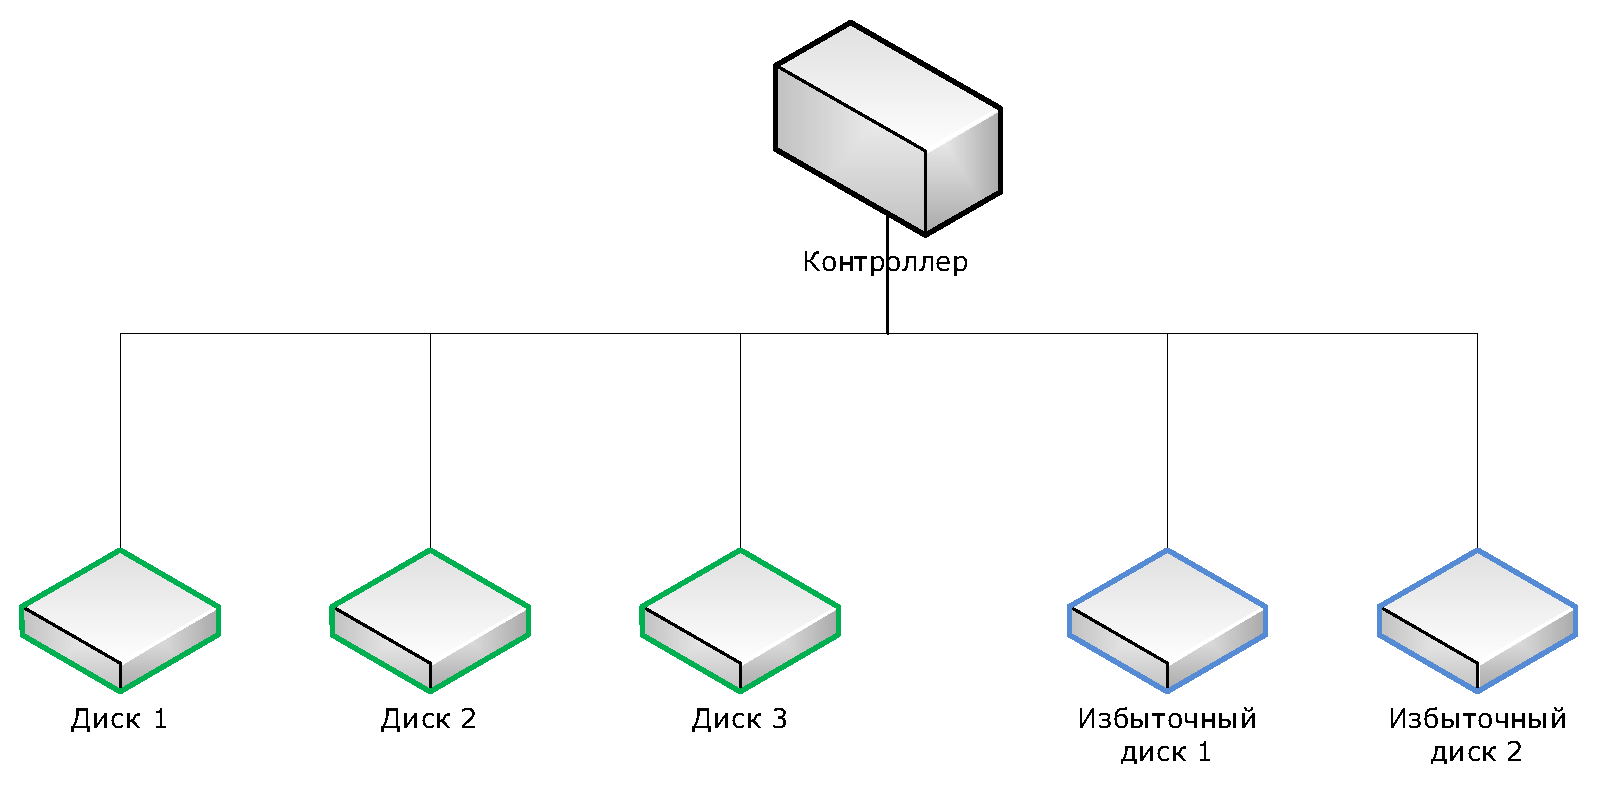
\includegraphics[width=0.7\linewidth]{pics/pic4_1_RAID-6.eps}}
\caption{Схема дискового массива RAID-6.}
\label{pic:4_1_RAID-6}
\end{figure}

Вероятность безотказной работы массива определяется по формуле:

$$P = 1 - \Bigr((1 - (1 - P_1)\cdot (1 - P_2))\cdot (1 - P_3)\Bigl)$$

Подставим значения вероятностей:
$$P = 1 - \Bigr(1 - (1 - 0.6)\cdot (1 - 0.6))\cdot (1 - 0.6)\Bigl)$$
$$P = 1 - 0.336 = 0.664$$

Таким образом, вероятность безотказной работы дисковой подсистемы сервера на базе RAID-6 равняется 0.664.

\subsection{Рекомендации по модернизации сети}

В центральном офисе и в первом филиале в сети используются устаревшие технологии: 10BASE-T и 10BASE-2. И если первую ещё можно модернизировать путём замены сетевых адаптеров и концентраторов с возможностью использования уже проложенного кабеля, то вторая потребует ещё и замены всего оборудования плюс демонтаж старого и прокладку нового кабеля.\par\bigskip

Если для работы фирмы достаточно текущей скорости передачи данных в сети и её пропускной способности, то не рекомендуется проводить модернизацию, так как это выльется в существенные финансовые и временные затраты.                    % Принципы построения сетей
%\newpage

\section{Организация связи с филиалами}

\subsection{Выбор технологии}

Мною было рассмотрено три варианта организации удалённых связей сети фирмы: X.25, Frame Relay и ADSL.\par\bigskip

Стандарт X.25, как правило используется для организации международных сетей. Для связи локальной сети с сетью X.25 используется мост или маршрутизатор. Доступ к сети осуществляется через арендуемую линию или линию с вызовом по номеру. В выделенных линиях обычно используют синхронную связь, что увеличивает пропускную способность. Скорость передачи составляет 19.2 - 64 Кбит/c. Линии с вызовом по номеру используют асинхронные методы с применением модемов, которые имеют собственные средства коррекции ошибок. Скорость передачи зависит от скорости модема.\par\bigskip

Поскольку стандарт X.25 предусмотрен для организации международных сетей, то и стоимость использования этой сети достаточно высока. При скорости 64 Кбит/c стоимость подключения составляет 30000 рублей, а абонентская плата - 4200 рублей в месяц.\par\bigskip

Сети Frame Relay - сравнительно новые сети, которые гораздо лучше подходят для передачи пульсирующего трафика локальных сетей по сравнению с сетями Х.25. Преимущество сетей Frame Relay заключается в их низкой протокольной избыточности и дейтаграммном режиме работы, что обеспечивает высокую пропускную способность и небольшие задержки кадров. Надежную передачу кадров технология Frame Relay не обеспечивает. Сети Frame Relay специально разрабатывались как общественные сети для соединения частных локальных сетей. Они обеспечивают скорость передачи данных до 2 Мбит/с.\par\bigskip

Услуги Frame Relay обычно предоставляются теми же провайдерами, которые эксплуатируют сети Х.25. Большая часть производителей выпускают сейчас коммутаторы, которые могут работать как по протоколам Х.25, так и по протоколам Frame Relay. Технология Frame Relay начинает занимать в территориальных сетях с коммутацией пакетов ту же нишу, которая заняла в локальных сетях технология Ethernet.\par\bigskip

Сети Frame Relay следует применять только при наличии на магистральных каналах волоконно-оптических кабелей высокого качества. Стоимость использования данной сети достаточно высока. Подключение стоит 57000 рублей и абонентская плата составляет 9000 рублей в месяц.\par\bigskip

ADSL модемы передают данные намного быстрее, чем обычные аналоговые модемы, используя те же телефонные линии. ADSL обеспечивает высокоскоростной широковещательный доступ. Скорость передачи данных достигает 8 Мб/с. ADSL работает по имеющейся телефонной линии и при этом не занимает телефонный канал. Таким образом, возможно одновременно пользоваться телефонным аппаратом и осуществлять доступ в интернет. Фактически, ADSL модем образует три канала:
\begin{itemize}
\item входящий канал, скорость до 8 Мбит/с, 
\item исходящий канал, скорость до 1 Мб/с, 
\item обычный канал телефонной связи, по которому ведутся телефонные разговоры.
\end{itemize}\par\bigskip

Скорость передачи данных зависит от используемого оборудования, длины и качества телефонной линии. ADSL не требует, как аналоговый модем, набора номера для установления соединения с сетью. Обычно, телефонные сервисы используют минимальную часть пропускной способности телефонной линии, ADSL занимает оставшуюся часть для реализации высокоскоростной передачи данных. Подключение стоит 3000 рублей, а абонентская плата составляет 1500 рублей в месяц.\par\bigskip

Качественные характеристики рассматриваемых технологий сведены в таблицу~\ref{table:ISP_compare_qual}.

\begin{table}[h]
\caption{Качественные характеристики технологий передачи данных}
\label{table:ISP_compare_qual}
\centering
  \begin{tabular}{|c|c|c|c|}
  \hline Параметр & X.25 & Frame Relay & ADSL \\
  \hline Скорость передачи, Кбит/с & 64 & 2000 & 8000 \\
  \hline Надёжность передачи данных & очень хорошая & отличная & хорошая \\
  \hline Возможность масштабирования & отличная & отличная & плохая \\
  \hline Стоимость подключения, рублей & 30000 & 57000 & 3000 \\
  \hline Абонентская плата, рублей & 4200 & 9000 & 1500 \\
  \hline
  \end{tabular}
\end{table}

Количественные характеристики рассматриваемых технологий сведены в таблицу~\ref{table:ISP_compare_numb}.

\begin{table}[h]
\caption{Количественные характеристики технологий передачи данных}
\label{table:ISP_compare_numb}
\centering
  \begin{tabular}{|c|c|c|c|}
  \hline Параметр & X.25 & Frame Relay & ADSL \\
  \hline Скорость передачи, Кбит/с & 64 & 2000 & 8000 \\
  \hline Надёжность передачи данных & 5 & 6 & 4 \\
  \hline Возможность масштабирования & 6 & 6 & 1 \\
  \hline Стоимость подключения, рублей & 30000 & 57000 & 3000 \\
  \hline Абонентская плата, рублей & 4200 & 9000 & 1500 \\
  \hline
  \end{tabular}
\end{table}

Теперь пронормируем параметры и добавим весовые коэффициенты. Результаты приведены в таблице~\ref{table:ISP_compare}.

\begin{table}[h]
\caption{Нормированные параметры рассматриваемых технологий}
\label{table:ISP_compare}
\centering
  \begin{tabular}{|c|c|c|c|c|}
  \hline Параметр & Коэфф. & X.25 & Frame Relay & ADSL \\
  \hline Скорость передачи, Кбит/с & 0.2 & 0.008 & 0.25 & 1 \\
  \hline Надёжность передачи данных & 0.3 & 0.833 & 1 & 0.666 \\
  \hline Возможность масштабирования & 0.2 & 1 & 1 & 0.166 \\
  \hline Стоимость подключения, рублей & 0.1 & 0.1 & 0.053 & 1 \\
  \hline Абонентская плата, рублей & 0.2 & 0.357 & 0.166 & 1 \\
  \hline Итог & 1 & 0.5329 & 0.5885 & 0.733 \\
  \hline
  \end{tabular}
\end{table}

Таким образом, выбор падает на технологию ADSL.

\subsection{Выбор оборудования}

\subsubsection{Выбор маршрутизатора}

Выбираем из трёх маршрутизаторов:
\begin{enumerate}
\item Asus RT-G32;
\item Cisco 2911R;
\item D-Link DIR-300.
\end{enumerate}

Качественные характеристики рассматриваемых маршрутизаторов сведены в таблицу~\ref{table:router_compare_qual}.

\begin{table}[h]
\caption{Качественные характеристики маршрутизаторов}
\label{table:router_compare_qual}
\centering
  \begin{tabular}{|c|c|c|c|}
  \hline Параметр & 1 & 2 & 3 \\
  \hline Количество портов & 4 & 8 & 12 \\
  \hline Сложность настройки & средняя & высокая & низкая \\
  \hline Размер таблицы маршрутизации & 10 & 20 & 25 \\
  \hline Гарантия, месяцев & 6 & 24 & 12 \\
  \hline Стоимость, рублей & 5000 & 8000 & 2000 \\
  \hline
  \end{tabular}
\end{table}

Количественные характеристики рассматриваемых маршрутизаторов сведены в таблицу~\ref{table:router_compare_numb}.

\begin{table}[h]
\caption{Количественные характеристики маршрутизаторов}
\label{table:router_compare_numb}
\centering
  \begin{tabular}{|c|c|c|c|}
  \hline Параметр & 1 & 2 & 3 \\
  \hline Количество портов & 4 & 8 & 12 \\
  \hline Сложность настройки & 2 & 1 & 3 \\
  \hline Размер таблицы маршрутизации & 10 & 25 & 20 \\
  \hline Гарантия, месяцев & 6 & 24 & 12 \\
  \hline Стоимость, рублей & 5000 & 8000 & 2000 \\
  \hline
  \end{tabular}
\end{table}

Теперь пронормируем параметры и добавим весовые коэффициенты. Результаты приведены в таблице~\ref{table:router_compare}.

\begin{table}[h]
\caption{Нормированные параметры маршрутизаторов}
\label{table:router_compare}
\centering
  \begin{tabular}{|c|c|c|c|c|}
  \hline Параметр & Коэфф. & 1 & 2 & 3 \\
  \hline Количество портов & 0.3 & 0.333 & 0.666 & 1 \\
  \hline Сложность настройки & 0.1 & 0.666 & 0.333 & 1 \\
  \hline Размер таблицы маршрутизации & 0.2 & 0.4 & 1 & 0.8 \\
  \hline Гарантия, месяцев & 0.2 & 0.25 & 1 & 0.5 \\
  \hline Стоимость, рублей & 0.2 & 0.4 & 0.25 & 1 \\
  \hline Итог & 1 & 0.3765 & 0.6831 & 0.86 \\
  \hline
  \end{tabular}
\end{table}

Таким образом, выбираем маршрутизатор D-Link DIR-300.

\subsubsection{Выбор модема}

Выбираем из трёх модемов:
\begin{enumerate}
\item D-Link DSL-2500U;
\item Asus DSL-N10;
\item Trendnet TDM-C504.
\end{enumerate}

Качественные характеристики рассматриваемых модемов сведены в таблицу~\ref{table:modem_compare_qual}.

\begin{table}[h]
\caption{Качественные характеристики модемов}
\label{table:modem_compare_qual}
\centering
  \begin{tabular}{|c|c|c|c|}
  \hline Параметр & 1 & 2 & 3 \\
  \hline Стандарты ADSL & ADSL, ADSL2, ADSL2+ & ADSL, ADSL2 & ADSL \\
  \hline Стандарты VPN & IPSec, PL2TP & IPSec, PPTP, PL2TP & IPSec \\
  \hline Flash-память, МБ & 4 & 8 & 20 \\
  \hline Гарантия, месяцев & 6 & 24 & 12 \\
  \hline Стоимость, рублей & 2000 & 3000 & 1500 \\
  \hline
  \end{tabular}
\end{table}

Количественные характеристики рассматриваемых модемов сведены в таблицу~\ref{table:modem_compare_numb}.

\begin{table}[h]
\caption{Количественные характеристики модемов}
\label{table:modem_compare_numb}
\centering
  \begin{tabular}{|c|c|c|c|}
  \hline Параметр & 1 & 2 & 3 \\
  \hline Стандарты ADSL & 3 & 2 & 1 \\
  \hline Стандарты VPN & 2 & 3 & 1 \\
  \hline Flash-память, МБ & 4 & 8 & 20 \\
  \hline Гарантия, месяцев & 6 & 24 & 12 \\
  \hline Стоимость, рублей & 2000 & 3000 & 1500 \\
  \hline
  \end{tabular}
\end{table}

Теперь пронормируем параметры и добавим весовые коэффициенты. Результаты приведены в таблице~\ref{table:modem_compare}.

\begin{table}[h]
\caption{Нормированные параметры модемов}
\label{table:modem_compare}
\centering
  \begin{tabular}{|c|c|c|c|c|}
  \hline Параметр          & Коэфф. & 1      & 2      & 3 \\
  \hline Стандарты ADSL    & 0.3    & 1      & 0.5    & 0.333 \\
  \hline Стандарты VPN     & 0.3    & 0.5    & 1      & 0.333 \\
  \hline Flash-память, МБ  & 0.1    & 0.2    & 0.4    & 1 \\
  \hline Гарантия, месяцев & 0.2    & 0.25   & 1      & 0.5 \\
  \hline Стоимость, рублей & 0.1    & 0.75   & 0.5    & 1 \\
  \hline Итог              & 1      & 0.545  & 0.74   & 0.4998 \\
  \hline
  \end{tabular}
\end{table}

Таким образом, выбираем модем Asus DSL-N10.

\subsubsection{Выбор сервера}

Выбираем из трёх серверов на базе 4 ядерных процессоров:
\begin{enumerate}
\item ASUS RS720-E6-R;
\item Dell E3-1240V2;
\item IBM KVR16E11/4.
\end{enumerate}

Выбор весовых коэффициентов параметров сравнения серверов будет проводиться с использованием метода анализа иерархий, а выбор сервера - с использованием метода взвешенной суммы параметров сравнения.

Качественные характеристики рассматриваемых серверов сведены в таблицу~\ref{table:server_compare_qual}.

\begin{table}[h]
\caption{Качественные характеристики серверов}
\label{table:server_compare_qual}
\centering
  \begin{tabular}{|c|c|c|c|}
  \hline Параметр & 1 & 2 & 3 \\
  \hline Частота процессора, ГГц & 2.4 & 3.4 & 3.1 \\
  \hline Оперативная память, ГБ & 12 & 10 & 16 \\
  \hline Жёсткий диск, ТБ & 2 & 4 & 1 \\
  \hline Блок питания, Вт & 500 & 700 & 650 \\
  \hline Горячая замена дисков & легко & непросто & затруднительно \\
  \hline Сетевой адаптер & LAN, WiFi & LAN & LAN, WiFi\\
  \hline Стоимость, рублей & 79000 & 39000 & 43000 \\
  \hline
  \end{tabular}
\end{table}

Количественные характеристики рассматриваемых серверов сведены в таблицу~\ref{table:server_compare_numb}.

\begin{table}[h]
\caption{Количественные характеристики серверов}
\label{table:server_compare_numb}
\centering
  \begin{tabular}{|c|c|c|c|}
  \hline Параметр                & 1     & 2     & 3 \\
  \hline Частота процессора, ГГц & 2.4   & 3.4   & 3.1 \\
  \hline Оперативная память, ГБ  & 12    & 10    & 16 \\
  \hline Жёсткий диск, ТБ        & 2     & 4     & 1 \\
  \hline Блок питания, Вт        & 500   & 700   & 650 \\
  \hline Горячая замена дисков   & 4     & 3     & 2 \\
  \hline Сетевой адаптер         & 3     & 2     & 3 \\
  \hline Стоимость, рублей       & 79000 & 39000 & 43000 \\
  \hline
  \end{tabular}
\end{table}

Весовые коэффициенты определяем методом анализа иерархий. Вычисление осуществляется посредством электронных таблиц MS Excel, которые находятся в приложении. Полученные результаты приведены в таблице~\ref{table:server_compare_veskoef}.

\begin{table}[h]
\caption{Весовые коэффициенты}
\label{table:server_compare_veskoef}
\centering
  \begin{tabular}{|c|c|c|c|c|c|c|c|c|c|}
  \hline    & К1    & К2    & К3    & К4  & К5 & К6    & К7   & Вектор & $\alpha$ \\
  \hline К1 & 1     & 1     & 2     & 4   & 6  & 4     & 5    & 2.67   & 0.284 \\
  \hline К2 & 1     & 1     & 2     & 4   & 6  & 4     & 5    & 2.67   & 0.284 \\
  \hline К3 & 0.5   & 0.5   & 1     & 3   & 5  & 4     & 4    & 1.79   & 0.192 \\
  \hline К4 & 0.25  & 0.25  & 0.333 & 1   & 2  & 1     & 0.5  & 0.57   & 0.061 \\
  \hline К5 & 0.167 & 0.167 & 0.2   & 0.5 & 1  & 0.333 & 0.25 & 0.3    & 0.032 \\
  \hline К6 & 0.25  & 0.25  & 0.25  & 1   & 3  & 1     & 0.5  & 0.59   & 0.062 \\
  \hline К7 & 0.2   & 0.2   & 0.25  & 2   & 4  & 2     & 1    & 0.77   & 0.082 \\
  \hline
  \end{tabular}
\end{table}

Проводим расчёт оценки согласованности. Для $m_f = 7$, $R = 1.32$:

$$\lambda_{max} = \sum_{i=1}^{m_f}\Bigr(a_i\cdot\sum_{j=1}^{m_f}x_{ij}\Bigl)=7.2566$$

$$\text{ОцСогл} = \frac{\lambda_{max} - m_f}{(m_f - 1)\cdot R} = \frac{8.5594 - 7}{(7 - 1)\cdot 1.32} = 0.056$$

Как видим, $0.056 < 0.1$, значит матрица согласована.\par\bigskip

Теперь пронормируем параметры и добавим весовые коэффициенты. Результаты приведены в таблице~\ref{table:server_compare}.

\begin{table}[h]
\caption{Нормированные параметры серверов}
\label{table:server_compare}
\centering
  \begin{tabular}{|c|c|c|c|c|}
  \hline Параметр                & Коэфф. & 1     & 2     & 3 \\
  \hline Частота процессора, ГГц & 0.284  & 0.706 & 1     & 0.911 \\
  \hline Оперативная память, ГБ  & 0.284  & 0.75  & 0.625 & 1 \\
  \hline Жёсткий диск, ТБ        & 0.192  & 0.5   & 1     & 0.25 \\
  \hline Блок питания, Вт        & 0.061  & 0.714 & 1     & 0.929 \\
  \hline Горячая замена дисков   & 0.032  & 1     & 0.75  & 0.5 \\
  \hline Сетевой адаптер         & 0.062  & 1     & 0.666 & 1 \\
  \hline Стоимость, рублей       & 0.082  & 0.494 & 1     & 0.907 \\
  \hline Итог                    & 1      & 0.59356 & 0.86179 & 0.79978 \\
  \hline
  \end{tabular}
\end{table}

Таким образом, выбираем сервер Dell E3-1240V2.

\subsubsection{Выбор ИБП для сервера}

Выбираем из трёх ИБП:
\begin{enumerate}
\item SVEN Power Pro+ 500 ;
\item PowerCom Warrior WAR-500A ;
\item Ippon Back Verso 400.
\end{enumerate}

Качественные характеристики рассматриваемых ИБП сведены в таблицу~\ref{table:ibp_compare_qual}.

\begin{table}[h]
\caption{Качественные характеристики ИБП}
\label{table:ibp_compare_qual}
\centering
  \begin{tabular}{|c|c|c|c|}
  \hline Параметр & 1 & 2 & 3 \\
  \hline Размеры & большой & средний & средний \\
  \hline Время реакции, мс & 10 & 4 & 6 \\
  \hline Автономная работа, мин & 8 & 10 & 13 \\
  \hline Время зарядки & 8 & 6 & 8 \\
  \hline Стоимость, рублей & 1500 & 1400 & 1700 \\
  \hline
  \end{tabular}
\end{table}

Количественные характеристики рассматриваемых ИБП сведены в таблицу~\ref{table:ibp_compare_numb}.

\begin{table}[h]
\caption{Количественные характеристики ИБП}
\label{table:ibp_compare_numb}
\centering
  \begin{tabular}{|c|c|c|c|}
  \hline Параметр & 1 & 2 & 3 \\
  \hline Размеры & 1 & 2 & 2 \\
  \hline Время реакции, мс & 10 & 4 & 6 \\
  \hline Автономная работа, мин & 8 & 10 & 13 \\
  \hline Время зарядки & 8 & 6 & 8 \\
  \hline Стоимость, рублей & 1500 & 1400 & 1700 \\
  \hline
  \end{tabular}
\end{table}

\newpage

Теперь пронормируем параметры и добавим весовые коэффициенты. Результаты приведены в таблице~\ref{table:ibp_compare}.

\begin{table}[h]
\caption{Нормированные параметры ИБП}
\label{table:ibp_compare}
\centering
  \begin{tabular}{|c|c|c|c|c|}
  \hline Параметр               & Коэфф. & 1      & 2      & 3 \\
  \hline Размеры                & 0.1    & 0.5    & 1      & 1 \\
  \hline Время реакции, мс      & 0.3    & 0.4    & 1      & 0.666 \\
  \hline Автономная работа, мин & 0.3    & 0.615  & 0.769  & 1 \\
  \hline Время зарядки, ч       & 0.2    & 0.75   & 1      & 0.75 \\
  \hline Стоимость, рублей      & 0.1    & 0.933  & 1      & 0.824 \\
  \hline Итог                   & 1      & 0.5978 & 0.9307 & 0.8322 \\
  \hline
  \end{tabular}
\end{table}

Таким образом, выбираем ИБП PowerCom Warrior WAR-500A.                      % Выбор оборудования сети
%\newpage

\section{Настройка рабочих параметров сетевой ОС}

Согласно ТЗ, в качестве сетевой ОС выбрана ОС MS Windows 7.\par\bigskip

Когда речь идет о подключении компьютера с Windows 7 к локальной сети, процесс настройки механизмов очень похож на аналогичный процесс в более ранних версиях ОС MS Windows. Имеются также и определенные отличия, например в использовании определенного типа сетевого расположения.\par\bigskip

Выбор сетевого расположения влияет на защиту операционной системы от возможных воздействий локальной сети, поэтому, если правильно подобрать тип расположения, это позволит получить большую защиту.\par\bigskip

Однако данный параметр критичен только в случае, когда компьютер функционирует в составе одноранговой сети и подключен к рабочей или домашней группе. Если же компьютер входит в состав сети, управляемой доменом, весь контроль над защитой компьютера от сетевых атак ложится "на плечи" домена. Поэтому остается только надеяться, что в домене используется соответствующее программное обеспечение, например антивирусная программа.\par\bigskip

\subsection{Выбор сетевого расположения}

Как уже было сказано ранее, Windows 7 позволяет использовать разные варианты сетевого размещения компьютера при работе в составе локальной сети. Выбор или смена сетевого размещения влечет за собой изменения в работе соответствующих механизмов операционной системы.\par\bigskip

Различают следующие варианты сетевого размещения:
\begin{itemize}
\item домашняя сеть. Это сетевое размещение подразумевает, что компьютер входит в состав небольшой локальной сети, участники которой вам знакомы и уровень доверия к которым вполне высокий, что позволяет не беспокоиться о сетевых угрозах. Данный вариант размещения автоматически устанавливается, когда происходит подключение к одной из домашних сетей, например организованных посредством Windows 7.
\item сеть предприятия, или Рабочая сеть. Данное сетевое размещение подразумевает, что компьютер входит в состав рабочей сети, размер которой не столь важен, главное – достаточный уровень доверия, что позволяет оценивать сеть как доверенную.
\item общественная сеть. Это сетевое размещение подразумевает подключение компьютера к случайной или непостоянной сети. Примером такой сети может стать зона Wi-Fi, например, в кафе или аэропорту. По понятным причинам данная сеть обладает наименьшей степенью доверия. При ее использовании активируются соответствующие механизмы защиты операционной системы.
\item доменная сеть. Наиболее доверенный тип сетевого размещения, выбор которого в обычном режиме недоступен. Смена на этот тип сетевого размещения происходит автоматически и только в том случае, когда выполняется подключение компьютера к сети с доменом.
\end{itemize}

Смену сетевого размещения можно производить самостоятельно либо оставить этот выбор на усмотрение операционной системы.\par\bigskip

Если требуется изменить сетевое размещение, воспользуйтесь для этого окном Центр управления сетями и общим доступом, запустить которое можно из Панели управления.

\subsection{Подключение к рабочей группе}

Для начала необходимо открыть механизм Система, запустить который можно с Панели управления. Здесь отображается некоторая информация о компьютере, а также сведения об имени компьютера и его текущей принадлежности к какой-либо сети. Кроме того, здесь находится механизм изменения этого состояния. Чтобы им воспользоваться, перейдите по ссылке Изменить параметры.\par\bigskip

В появившемся окне отображается описание компьютера, его имя и рабочая группа или домен, к которому он принадлежит. Здесь же присутствуют две кнопки, позволяющие подключить компьютер к рабочей группе или домену.\par\bigskip

Для подключения компьютера к рабочей группе щелкните на кнопке Изменить.\par\bigskip

Чтобы подключить компьютер к нужной рабочей группе, достаточно просто ввести ее название в соответствующее поле и нажать кнопку OK. Никакой авторизации при этом не требуется, поскольку сам принцип организации работы рабочей группы подразумевает свободное членство в группе. Буквально через несколько секунд появится окно с подтверждение того, что компьютер подключен к рабочей группе. Вам остается только перезагрузить компьютер, чтобы начать полноценную работу уже в составе этой рабочей группы.

\subsection{Подключение к домену}

Подключение к домену компьютера с операционной системой Windows 7, как и в других операционных системах, требует определенных прав доступа (точнее, прав на подключение компьютера к домену). Кроме того, потребуются данные об учетной записи пользователя, который будет работать на этом компьютере. В этом нет ничего странного, поскольку уровень безопасности в доменной сети подразумевает максимально возможную защиту как вашего компьютера, так и управляющего сервера, который организует работу сети. Процесс подключения к домену, а также добавления сетевого пользователя контролирует мастер подключений.\par\bigskip

Первое, что предстоит сделать, – выбрать направление работы мастера. Мастер универсален: он позволяет подключать компьютер не только к домену, но и к рабочей группе, поэтому, чтобы направить его усилия «в нужное русло», требуется указать соответствующий вариант действий. Выбор очевиден, поэтому, установив переключатель в положение с упоминанием корпоративной сети, продолжаем работу мастера.\par\bigskip

Поскольку наша задача – подключение к домену, выберите соответствующее положение переключателя, в результате чего процесс подключения продолжится.\par\bigskip

Далее мастер вас предупредит, что для подключения к домену нужна определенная информация. В частности, сведения об учетных данных сетевого пользователя, который будет работать на данном компьютере, а также имя компьютера, под которым он будет идентифицирован в сети, если данные о нем не будут найдены в Active Directory. Подготовив эту информацию, продолжите процесс. При этом следует учитывать, что учетная запись пользователя уже должна быть зарегистрирована в Active Directory, иначе подключение будет невозможно.\par\bigskip

Если авторизация будет успешной, появится окно, сообщающее, что для завершения процесса подключения требуется перезагрузка компьютера. В противном случае необходимо будет уточнить данные авторизации либо отказаться от подключения к домену.\par\bigskip

\subsection{Настройка TCP/IP-протокола}

Настройка параметров TCP/IP-протокола требуется в том случае, когда необходимо изменить способ IP-адресации, а также уточнить IP-адреса DNS-серверов и добавить маршруты. Изменить настройки протокола очень просто, и, что самое главное, это можно сделать "на ходу", то есть без перезагрузки компьютера.\par\bigskip

Для выполнения необходимых изменений будем использовать Центр управления сетями и общим доступом, открыть который можно с Панели управления.\par\bigskip

В правой части появившегося окна находится несколько ссылок, позволяющих получить доступ к разным функциям. В частности, чтобы получить доступ к настройкам сетевого адаптера, необходимо использовать ссылку Изменение параметров адаптера. При её нажатии откроется окно, содержащее список всех сетевых подключений, которые используются на компьютере.\par\bigskip

Из всего списка служб и протоколов, которые обслуживают нужное нам сетевое подключение, нас интересует строка Протокол Интернета версии 4 (TCP/IPv4). Дважды щелкните на ней. Появится окно настройки TCP/IP-протокола. Здесь вы можете вносить все необходимые изменения, но главное не ошибиться, поскольку от этого зависит, будет ли компьютер виден в сети.                          % Настройка сетевой ОС
%\newpage

\section{Настройка рабочих параметров СУБД}

Согласно ТЗ, в качестве СУБД используется СУБД Sybase от одноимённой компании.

\subsection{Инсталляция}

На сервере должно быть установлено сетевое программное обеспечение: сетевой протокол (например, TCP/IP, NetBEUI или SPX/IPX), клиентская часть для работы в сети (Client for Microsoft Networks) для машин на Intel платформе. Для использования протокола TCP/IP серверу должен быть присвоен уникальный IP-адрес. Проверка правильности установки протокола TCP/IP может быть произведена с помощью команды: \verb|ping <servername>|, запущенной с любой другой машины в сети. При правильной настройке будет получен ответ: \verb|Replay from ...|\par\bigskip

Сначала создается глобальная переменная среды SYBASE, которой присваивается значение каталога, в который производится установка, например:

\verb|D:\SYBASE|.\par\bigskip

Запуск инсталляции производится с помощью команды setup.exe с CD-диска, если он не начался автоматически после вставки инсталляционного диска в CD-ROM.\par\bigskip

Важным моментом при инсталляции является выбор кодовой страницы и порядка сортировки, а также номер порта, по которому будет осуществляться взаимодействие клиентских приложений с ASE по протоколу TCP/IP. Номер порта может быть изменен впоследствии только при переустановке Sybase ASE. Рекомендуемые значения параметров для кодовой страницы и порядка сортировки: Character Set - 1251 (id=53), Sort Order - Case Insensitive, Accent Sensitive (id=59).\par\bigskip

\subsection{Установка параметров и настройка}

Полный список всех параметров вызывается с помощью системной процедуры \verb|sp_configure| и хранится в системной таблице \verb|sysconfigures|. Часть параметров после изменения не требует перезапуска сервера, так как являются динамическими. Чтобы проверить, требуется ли перезапуск сервера после изменения значения параметра, нужно сравнить значения \verb|config_value| и \verb|run_value|, возвращаемые командой:

\verb|sp_configure <имя_параметра>|\par\bigskip

При равенстве этих значений перезапуск не требуется. Для изменения значения параметра используется команда:

\verb|sp_configure <имя_параметра>, <новое_значение>|\par\bigskip

Далее приводятся основные параметры настройки.\par\bigskip

\verb|Allow updates to system tables = 0|

Запрещено обновление системных таблиц. Выполняется для предотвращения случайного изменения таблиц пользователями. Параметр может быть временно сделан равным 1 при необходимости изменения системных таблиц администратором системы, после чего снова обязательно должен быть обнулен.\par\bigskip

\verb|Deadlock checking period = 5000|

Время в миллисекундах, после прохождения которого ожидающий освобождения ресурса процесс признается deadlock'ом. Увеличение значения параметра по сравнению со значением по умолчанию позволяет сократить количество проверок deadlock'ов в единицу времени и избежать ошибочных присвоений ожидающим процессам статуса deadlock.\par\bigskip

\verb|Default character set id = 53|

Устанавливается кодовая страница cp1251, поддерживающая русский язык. Значение параметра устанавливается в процессе инсталляции сервера, и при изменении его с помощью команды \verb|sp_configure| требуется либо предварительная выгрузка и повторная загрузка всех баз данных из-за изменения формата хранения данных, либо проведение ряда административных мероприятий после автоматической конвертации баз.\par\bigskip

\verb|Default sort order id = 59|

По аналогии с предыдущим параметром устанавливается алфавитный регистронезависимый порядок сортировки. Оба эти параметра рекомендуется устанавливать сразу при инсталляции системы до создания рабочих баз данных.\par\bigskip

\verb|Lock scheme = datapages|

Устанавливает тип блокировки для создаваемых таблиц по умолчанию в значение 'datapages' (постраничная блокировка).\par\bigskip

\verb|Max online engines = n|

Устанавливается количество логических процессоров, которое будет предоставлено Sybase для обработки запросов.\par\bigskip

\verb|Number of devices = n|

По умолчанию значение этого параметра = 10. Если на сервере необходимо создать больше устройств баз данных, то это можно сделать, соответственно увеличив значение параметра.\par\bigskip

\verb|Number of locks = 50000|

Количество блокировок, которые одновременно могут быть установлены процессами всех работающих пользователей.\par\bigskip

\verb|Number of open databases = n|

Устанавливается по количеству реально существующих баз данных на сервере, включая системные и пользовательские базы.\par\bigskip

\verb|Number of open indexes = 2009|

Количество одновременно открытых индексов.\par\bigskip

\verb|Number of open objects = 50000|

Количество одновременно открытых объектов баз данных.\par\bigskip

\verb|Number of user connections = users|

Значение параметра должно соответствовать увеличенному в пять раз количеству пользователей, которые могут одновременно работать на сервере.\par\bigskip

\verb|Page lock promotion HWM = 20000|

Пороговое значение, определяющее, после какого количества страничных блокировок в таблице к ней будет применена полная блокировка.\par\bigskip

\verb|Row lock promotion HWM = 20000|

Пороговое значение, определяющее, после какого количества позаписных блокировок в таблице к ней будет применена полная блокировка.\par\bigskip

\verb|User log cache size = 4096|

Размер пользовательского буфера транзакций, в который накапливаются транзакции перед записью в transaction log. Увеличение этого параметра позволяет уменьшить количество конфликтов, возникающих при одновременной попытке нескольких процессов выполнить запись в transaction log.\par\bigskip

Кроме того, в файле \verb|%SYBASE%\locales\locales.dat| нужно для секции \verb|[nt]| заменить строки:
\begin{verbatim}
locale = enu, us_english, iso_1
locale = default, us_english, iso_1
\end{verbatim}
на:
\begin{verbatim}
locale = enu, us_english, cp1251
locale = default, us_english, cp1251
\end{verbatim}                           % Настройка СУБД
%\newpage

\section{Распределение предметных БД по узлам сети}

Согласно ТЗ, необходимо распределить предметные БД по узлам сети без учёта репликации. В настоящем документе приведены результаты вычислений, которые осуществлялись посредством электронных таблиц MS Excel. Соответствующие документы находятся в приложении.\par\bigskip

Необходимо определить вариант рационального размещения предметных баз данных в распределенной информационной системе для случая, когда каждая база данных размещается только в одном узле сети, а обрабатывающие процессы (приложения) не являются распределенными. При этом следует считать, что если некоторый процесс обращается за данными к базе, находящейся в другом узле, сетевые затраты на одно обращение составляют $t$ секунд, независимо от местонахождения узла в сети и дисциплины обслуживания. Если процесс обращается к базе данных, находящейся в том же узле, где выполняется процесс, то следует считать, что $t = 0$.

Таблица~\ref{table:db_usage} показывает использование предметных баз данных обрабатывающими процессами (приложениями) в течение временного интервала и интенсивности их обращений к базам данных (среднее число обращений за рассматриваемый интервал времени).

\begin{table}[h]
\caption{Использование предметных баз данных}
\label{table:db_usage}
 \begin{tabular}{c}
 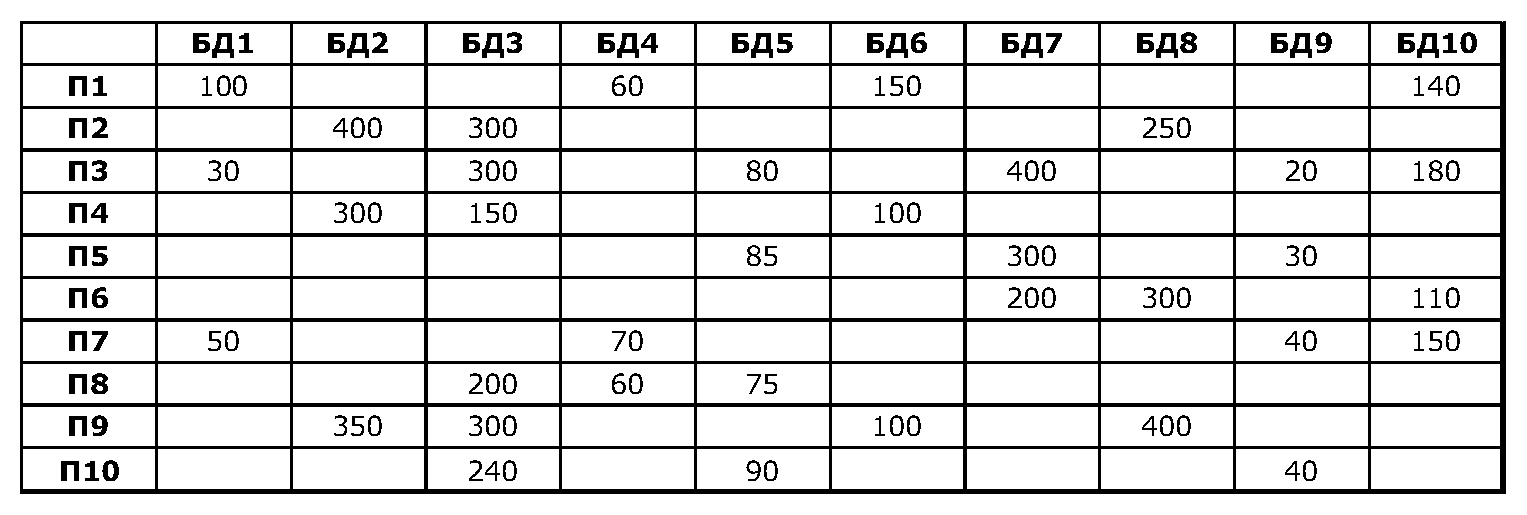
\includegraphics[width=1\linewidth]{pics/pic8_1_db_usage.eps}
 \end{tabular}
\end{table}

\newpage

Таблица~\ref{table:proc_distrib} показывает распределение обрабатывающих процессов по узлам распределённой сети.

\begin{table}[h]
\caption{Распределение обрабатывающих процессов по узлам}
\label{table:proc_distrib}
 \begin{tabular}{c}
 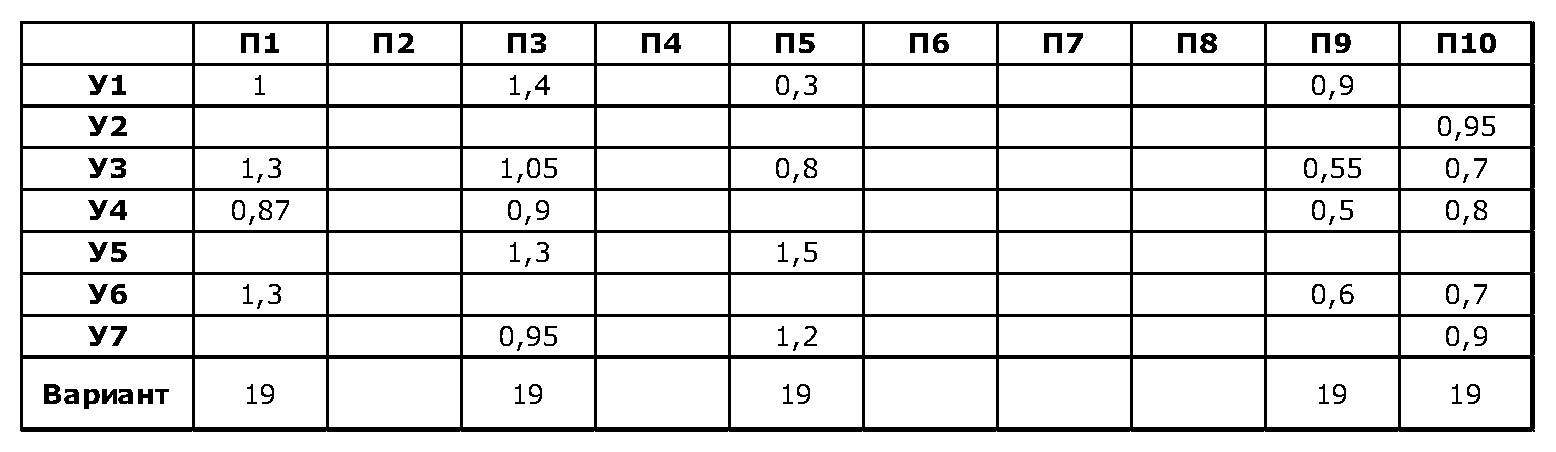
\includegraphics[width=1\linewidth]{pics/pic8_2_proc_disrib.eps}
 \end{tabular}
\end{table}

Коэффициенты в таблице~\ref{table:proc_distrib} используются для получения количества обращений к базе данных в исходном варианте задания по формуле:

$$N_1 = N\cdot k$$
где:\\
$N$ -– значение из таблицы~\ref{table:db_usage};\\
$k$ –- значение коэффициента из таблицы~\ref{table:proc_distrib};\\
$N_1$ -- результирующее значение для таблицы учебного варианта задания.\par\bigskip

\newpage

На основании данных из таблицы~\ref{table:db_usage} и таблицы~\ref{table:proc_distrib} для исходного варианта была сформирована сводная таблица исходных данных -- таблица~\ref{table:results}. Каждое значение этой таблицы есть среднее количество обращений к базе данных (БД$_i$) определенного процесса (П$_j$) из определенного узла сети (У$_k$).

\begin{table}[h]
\caption{Результаты затрат на обработку конкретной БД конкретными процессами в конкретных устройствах без учёта репликации}
\label{table:results}
 \begin{tabular}{c}
 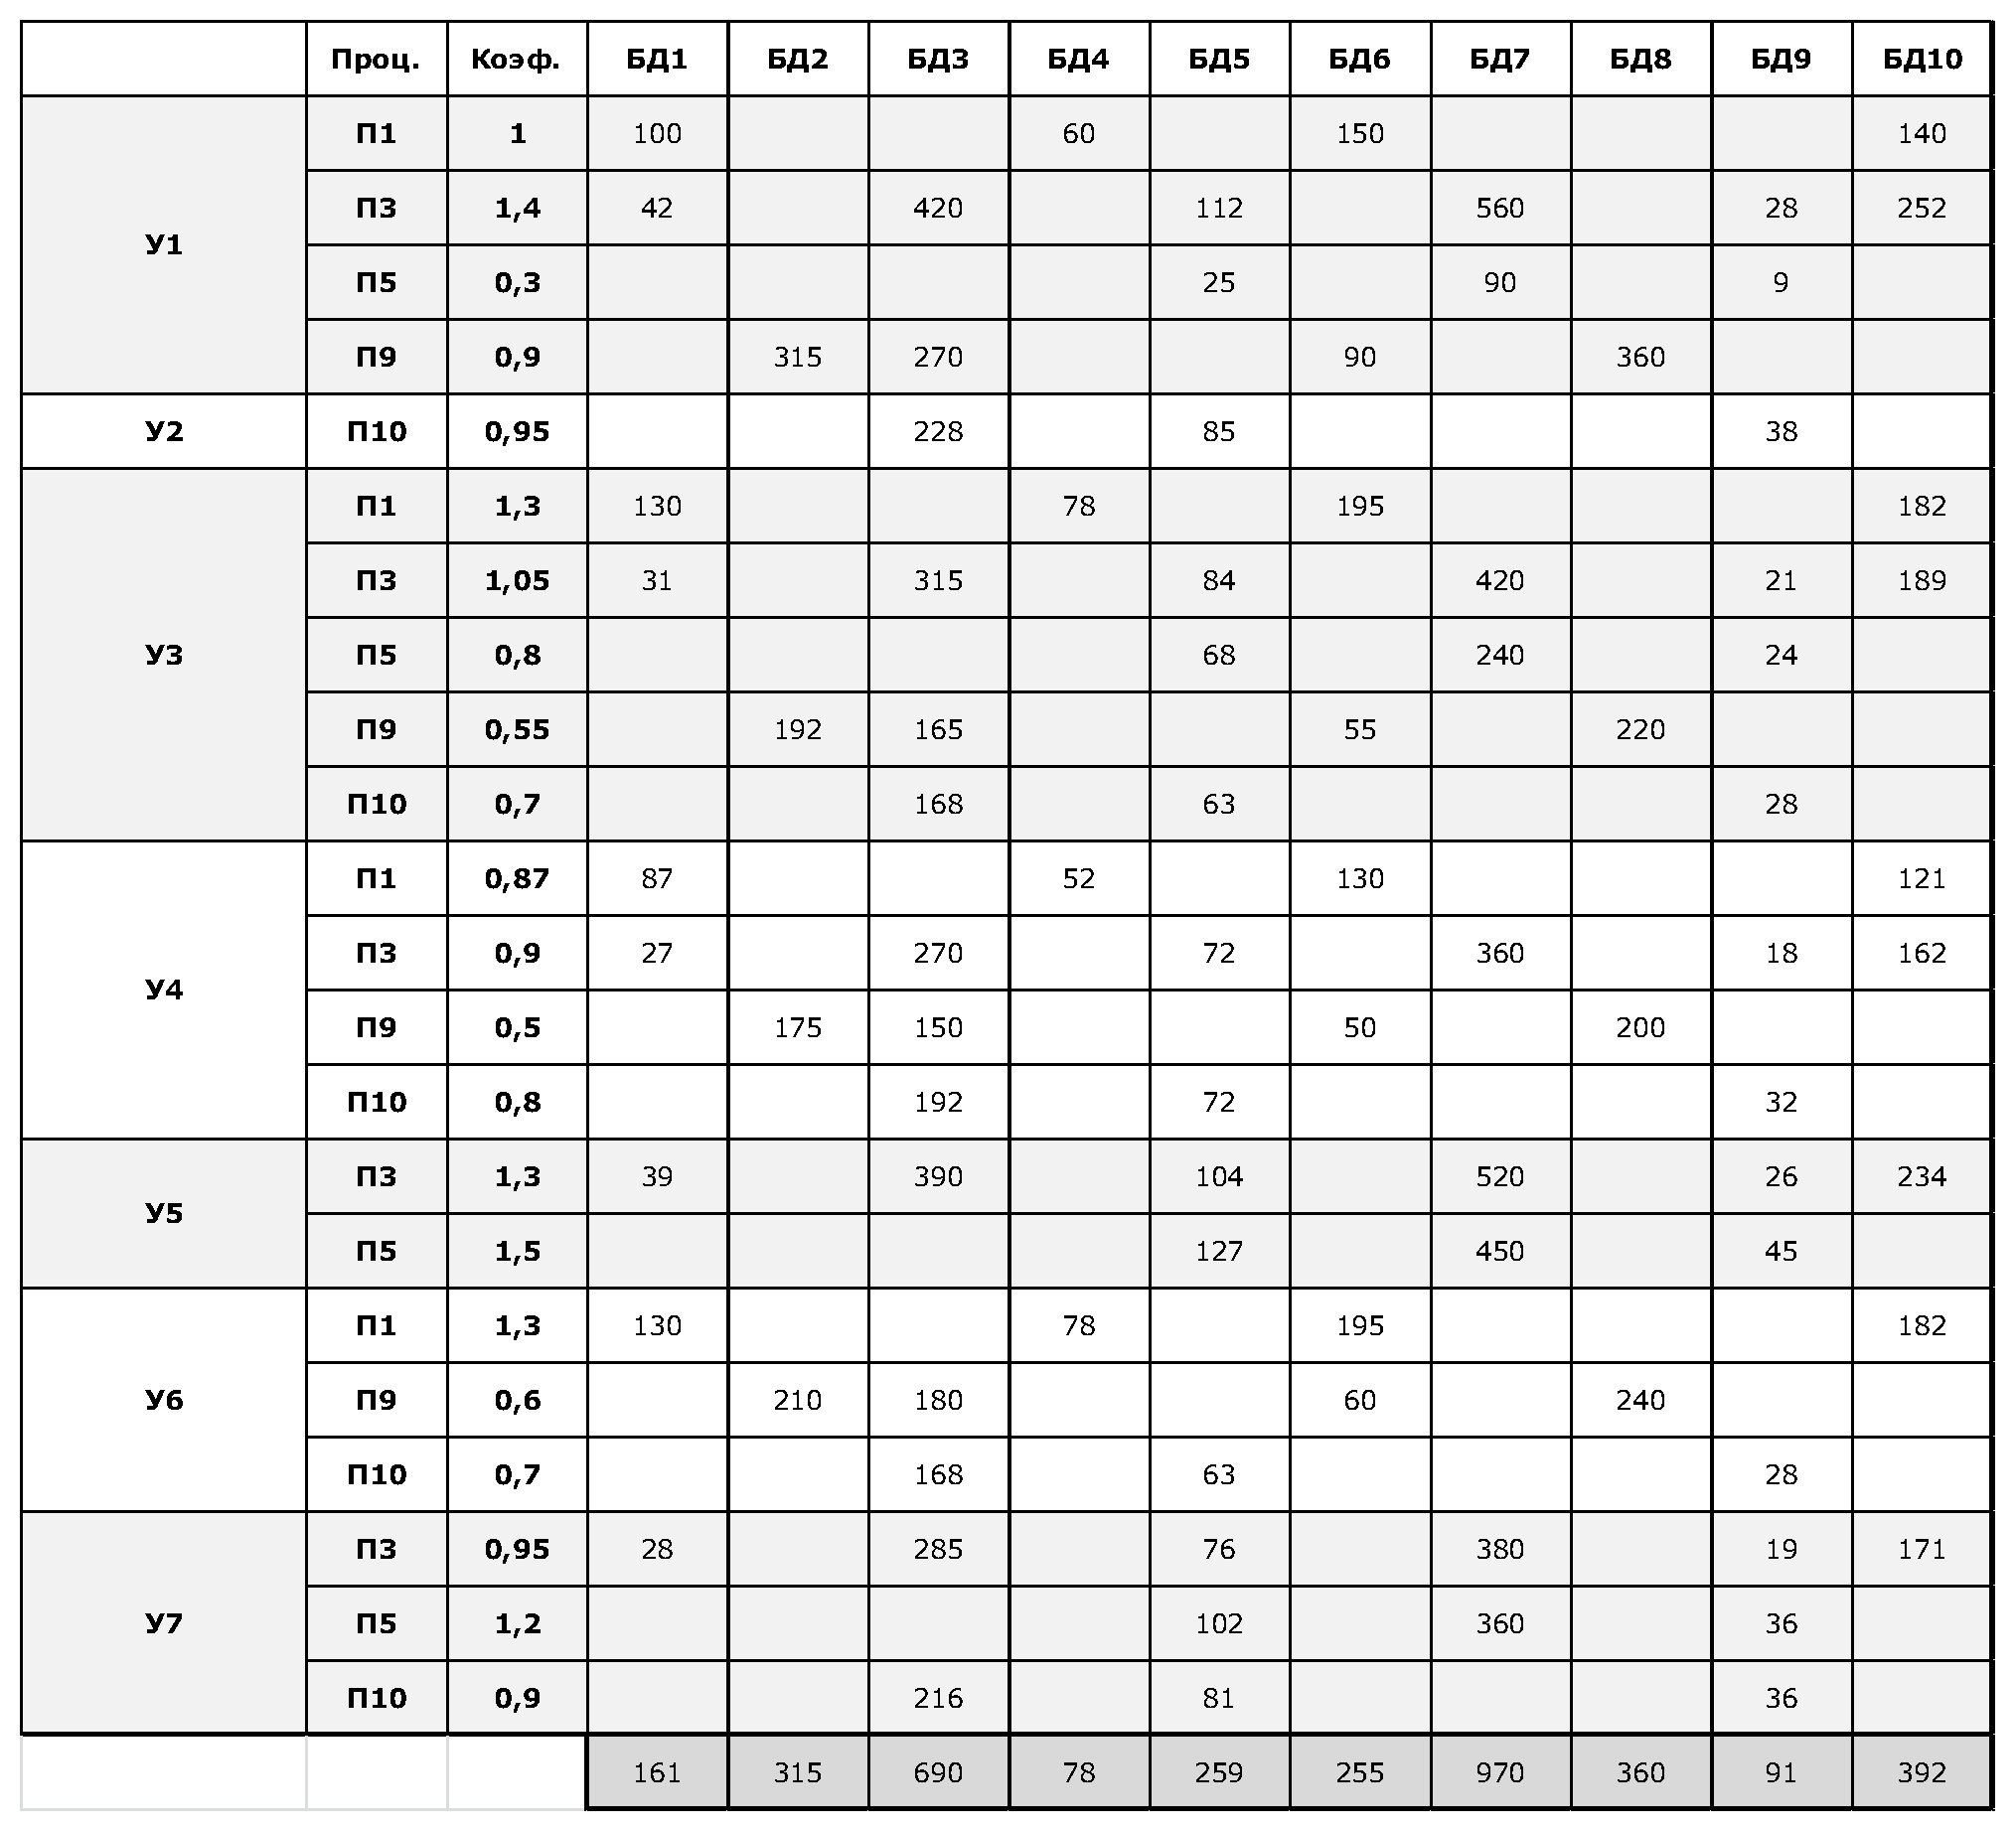
\includegraphics[width=1\linewidth]{pics/pic8_3_results.eps}
 \end{tabular}
\end{table}

\newpage

Составляем таблицу~\ref{table:sum_req}, в которой указываем все возможные варианты размещения баз данных по узлам сети. В каждую клетку этой таблицы записываем число, которое определяет суммарное количество всех запросов от всех процессов всех узлов к данной БД, при условии, что эта БД находится в данном узле.

\begin{table}[h]
\caption{Суммарное количество обращений к БД при возможных вариантах их размещения по узлам сети}
\label{table:sum_req}
 \begin{tabular}{c}
 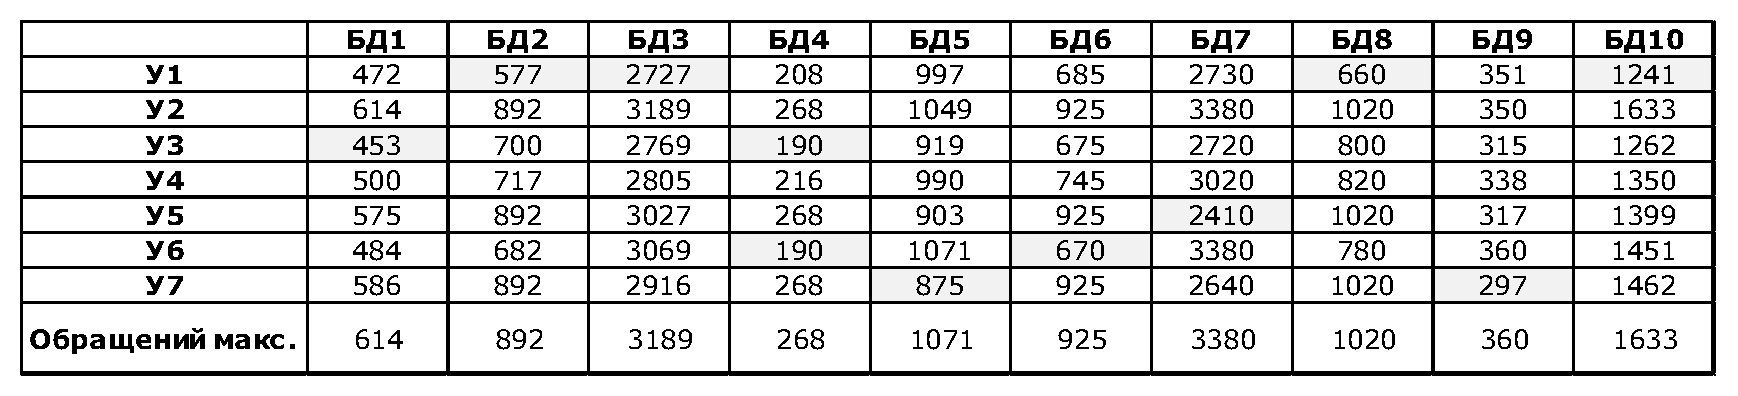
\includegraphics[width=1\linewidth]{pics/pic8_4_sum_req.eps}
 \end{tabular}
\end{table}

Используем правило: "Базу данных помещаем в тот узел, где она максимально используется, то есть суммарное количество обращений к ней со стороны других узлов минимально". Поэтому в каждом столбце, соответствующем одной конкретной БД, отыскиваем наименьшее значение. Это и будет соответствовать оптимальному варианту размещения этой БД, поскольку чем меньше это значение, тем меньше суммарное количество обращений от всех процессов всех других узлов к данной БД.\par\bigskip

Полученные результаты, показывающие оптимальные варианты размещения БД по узлам сети, записываем в таблицу~\ref{table:optimum}.

\begin{table}[h]
\caption{Оптимальные варианты размещения БД по узлам сети}
\label{table:optimum}
 \begin{tabular}{c}
 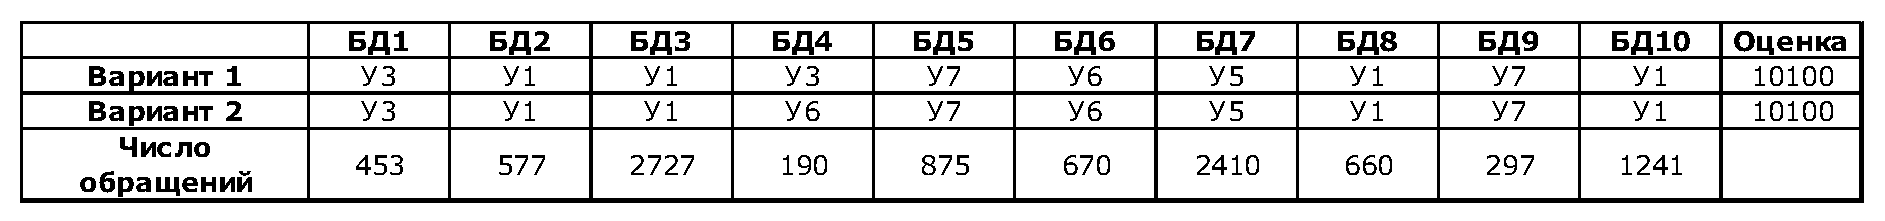
\includegraphics[width=1\linewidth]{pics/pic8_5_optimum.eps}
 \end{tabular}
\end{table}

Итак, получили, что в каждом из двух оптимальных вариантов размещения БД по узлам сети суммарное количество обращений ко всем БД, то есть суммарные затраты, составляет 10100.                     % Распределение БД по узлам
%\newpage

\section{Моделирование сети}

Необходимо выполнить аналитическое моделирование системы, содержащей 19 рабочих станций и сервер (ЦП и диски).\par\bigskip

Общая формализованная схема PCOD в виде сети массового обслуживания (СМО) приведена на рисунке~\ref{pic:9_1_model_general}.

\begin{figure}[h]
\center{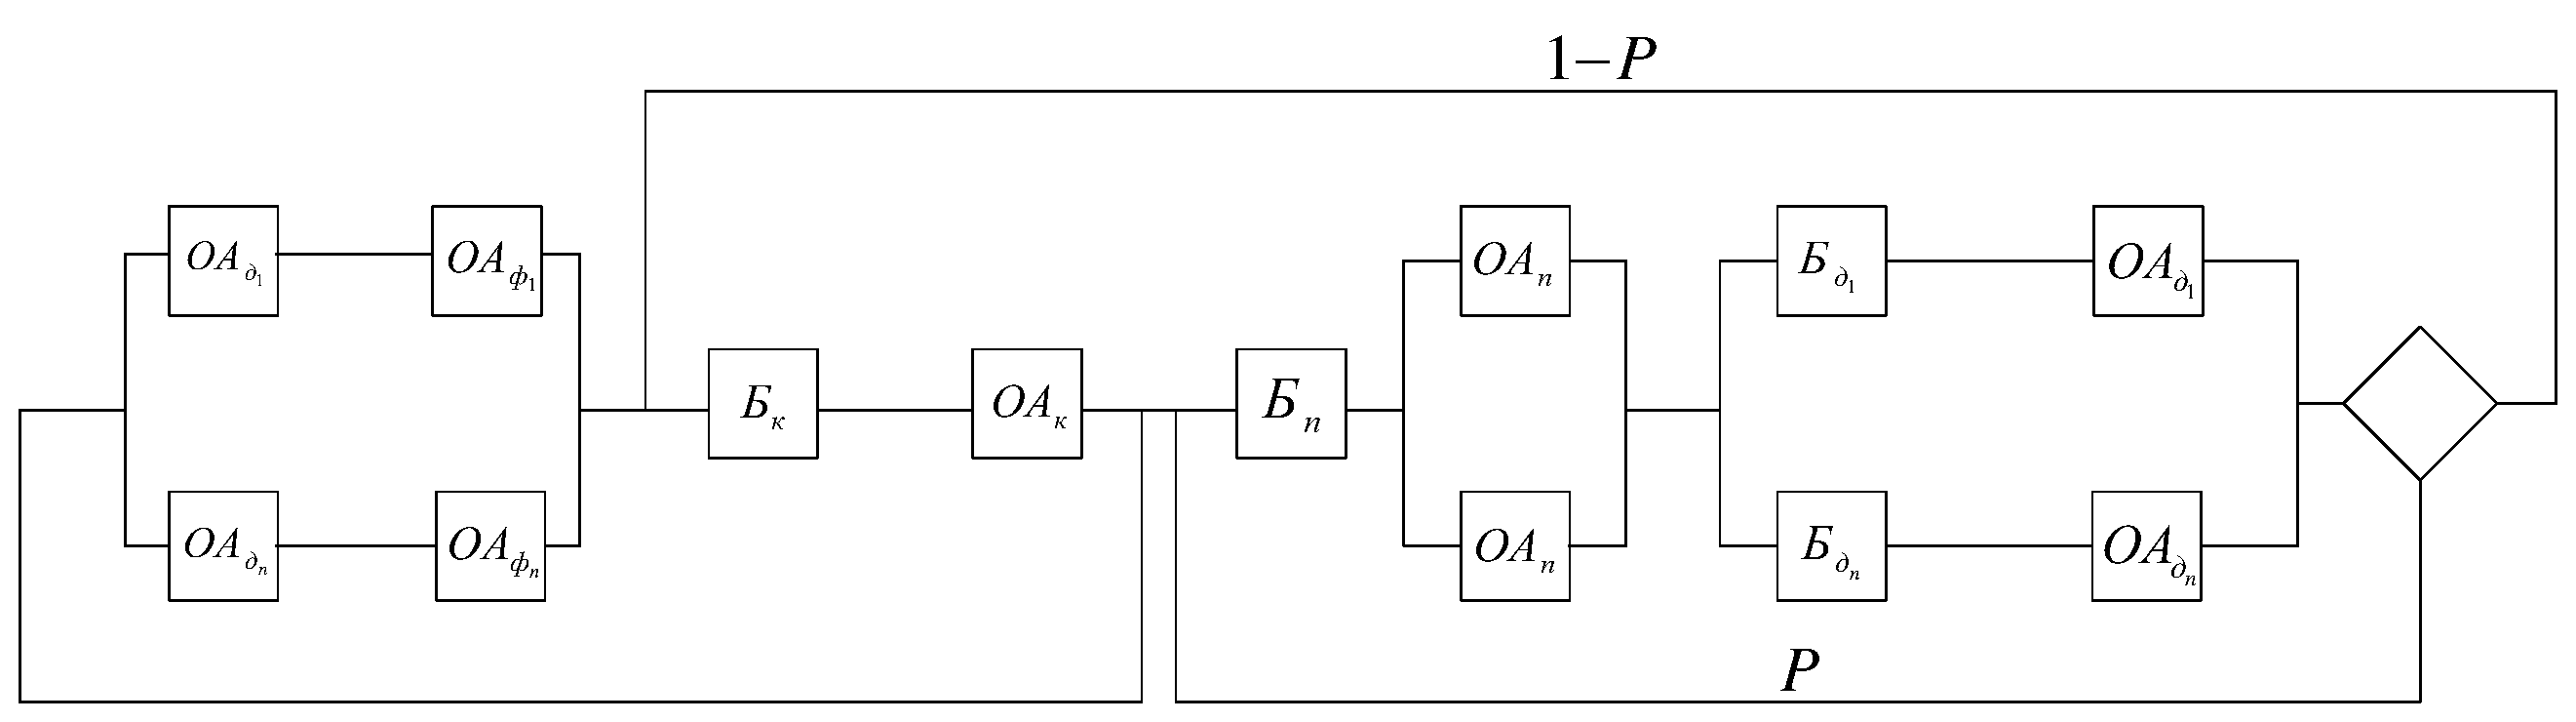
\includegraphics[width=1\linewidth]{pics/pic9_1_model_general.eps}}
\caption{Формализованная схема, содержащая ПЭВМ, канал и сервер (два ЦП и диски).}
\label{pic:9_1_model_general}
\end{figure}

В схеме используются следующие обозначения:\\
$\text{ОА}_{\text{д}_i}$ -- обслуживающий аппарат, имитирующий дообработку на $i$-той рабочей станции сети запроса от этой станции к серверу после обработки запроса на сервере;\\
$\text{ОА}_{\text{ф}_i}$ -- обслуживающий аппарат, имитирующий формирование запроса от $i$-той рабочей станции к серверу ($i = \overline{1..N}$);\\
$\text{Б}_{\text{к}}$ -- буфер, имитирующий очередь запросов к каналу;\\
$\text{ОА}_{\text{к}}$ -- обслуживающий аппарат, имитирующий задержку при передаче данных через канал;\\
$\text{Б}_{\text{п}}$ -- буфер, имитирующий очередь запросов к процессорам;\\
$\text{ОА}_{\text{п}}$ -- обслуживающие аппараты, имитирующие работу процессоров;\\
$\text{Б}_{\text{д}_i}$ -- буфер, имитирующий очередь запросов к $i$-му диску;\\
$\text{ОА}_{\text{д}_i}$ -- обслуживающий аппарат, имитирующий работу $i$-го диска;\\
$P$ -- вероятность обращения запроса к ЦП после обработки на диске. Обслуживание заявок во всех ОА подчиняется экспоненциальному закону.\par\bigskip

Формализованная схема рассматриваемой РСОД в виде CMO приведена на рисунке~\ref{pic:9_2_model_mine}.

\begin{figure}[h]
\center{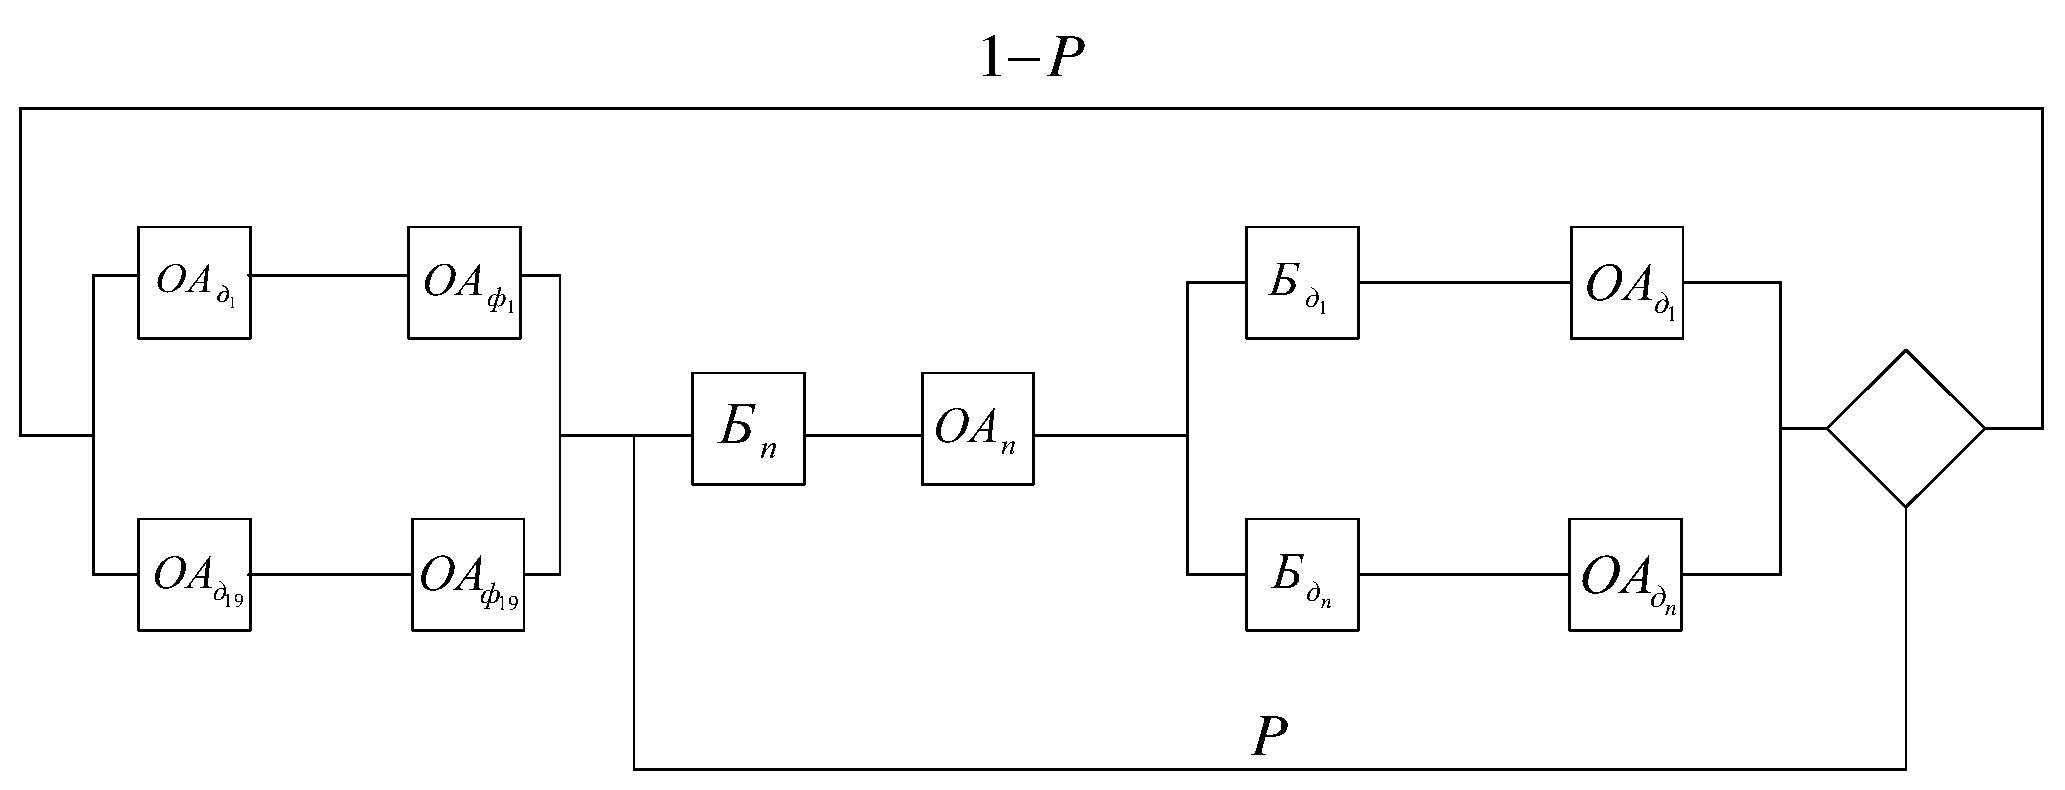
\includegraphics[width=1\linewidth]{pics/pic9_2_model_mine.eps}}
\caption{Формализованная схема рассматриваемой модели (ПЭВМ, сервер и диски).}
\label{pic:9_2_model_mine}
\end{figure}

Исходные данные модели представлены в таблице~\ref{table:in_data}.

\begin{table}[h]
\caption{Исходные данные модели}
\label{table:in_data}
\centering
 \begin{tabular}{|m{0.025\linewidth}|m{0.9\linewidth}|}
 \hline $N$ & число рабочих станций сети \\
 \hline $T_{\text{о}}$ & среднее значение времени дообработки на рабочей станции сети запроса от этой станции к базе данных на сервере \\
 \hline $T_{\text{р}}$ & среднее значение времени формирования запроса от рабочей станции сети к базе данных на сервере \\
 \hline $t_{\text{к}}$ & среднее значение времени передачи запроса по каналу \\
 \hline $\text{С}$ & число процессоров сервера \\
 \hline $t_{\text{пр}}$ & среднее значение времени обработки запроса в ЦП сервера \\
 \hline $t_{\text{д}_i}$ & среднее значение времени обработки запроса в диске сервера \\
 \hline $P_i$ & вероятность обращения запроса к $i$-му диску сервера после обработки запроса в процессоре \\
 \hline
 \end{tabular}
\end{table}

Выходные данные модели представлены в таблице~\ref{table:out_data}.

\begin{table}[h]
\caption{Выходные данные модели}
\label{table:out_data}
\centering
 \begin{tabular}{|m{0.05\linewidth}|m{0.9\linewidth}|}
 \hline $T_{\text{реак}}$ & среднее значение времени реакции системы \\
 \hline $\rho_{\text{к}}$ & коэффициент загрузки ОА, имитирующего работу канала передачи данных \\
 \hline $\rho_{\text{пр}}$ & коэффициент загрузки ОА, имитирующего работу процессора сервера \\
 \hline $\rho_{\text{д}_i}$ & коэффициент загрузки ОА, имитирующего работу i–ого диска сервера \\
 \hline
 \end{tabular}
\end{table}                          % Исходные данные моделирования
%\newpage

\subsection{Аналитическое моделирование}

Введём следующие обозначения: \\
$\lambda_{\text{ф}_1}$ -- среднее значение суммарной интенсивности фонового потока запросов, выходящих из ОА, имитирующих работу рабочих станций, в канал; \\
$\lambda_{\text{ф}_1}\beta$ -- среднее значение интенсивности фонового потока запросов, проходящих через ОА, имитирующих работу сервера и дисков, где $\beta=\frac{1}{1 - P}$; \\
$\beta$ -- среднее количество проходов запроса по тракту процессор-диски за время одного цикла его обработки в системе; \\
$t_{\text{к}} = 0.5\cdot(t_{\text{к}_1} + t_{\text{к}_2})$ -- среднее значение времени обработки запроса в канале передачи данных, где $t_{\text{к}_1}$ и $t_{\text{к}_2}$ -- соответственно среднее время передачи запроса по каналу в прямом и обратном направлениях;
$n$ -- количество серверов, обслуживающих рабочие станции; \\
$m = \frac{1}{P_i}$ -- количество дисков в сервере, при условии, что все они одинаковые; \\
$P_i$ -- вероятность обращения к $i$-му диску сервера.\par\bigskip

При расчете используется приближённый итерационный алгоритм нахождения значения выходных характеристик рассматриваемой системы:
\begin{enumerate}

\item Определяем начальное значение для $\lambda_{\text{ф}_1}$: \\
 $$\lambda_{\text{ф}_1} = K_1min\left\{\frac{1}{2\cdot t_{\text{к}}};\frac{\text{С}}{\beta\cdot t_{\text{пр}}};\frac{1}{\beta\cdot P_i\cdot t_{\text{д}}}\right\}\cdot\frac{N - 1}{N}$$ \\
 $K_1$ принимает значения в диапазоне 0.995...0.99995.\par
 Определяем средние времена пребывания запроса в узлах системы (канале, процессоре, дисках): \\
 $$T_{\text{к}} = \frac{2\cdot t_{\text{к}}}{1 - 2\cdot\lambda_{\text{ф}_1}\cdot t_{\text{к}}}$$
 $$T_{\text{пр}} = \frac{\beta\cdot t_{\text{пр}}}{1 - (\beta\cdot\lambda_{\text{ф}_1}\cdot\frac{t_{\text{пр}}}{\text{С}})^{\text{С}}}$$
 $$T_{\text{д}} = \frac{\beta\cdot t_{\text{д}}}{1 - \beta\cdot P_i\cdot\lambda_{\text{ф}_1}\cdot t_{\text{д}}}$$
 
\item Определяем интенсивность фонового потока после очередной итерации:
 $$\lambda_{\text{ф}} = \frac{N - 1}{T_{\text{о}} + T_{\text{р}} + T_{\text{к}} + T_{\text{пр}} + T_{\text{д}}}$$
 
\item Сравниваем $\lambda_{\text{ф}_1}$ и $\lambda_{\text{ф}}$. Если $\frac{|\lambda_{\text{ф}_1} - \lambda_{\text{ф}}|}{\lambda_{\text{ф}}} < \Delta_1$, то переход на пункт 5, иначе на 4;

\item Определяем новое приближённое значение для $\lambda_{\text{ф}_1}$:
 $$\delta_1 = \frac{\lambda_{\text{ф}_1} - \lambda_{\text{ф}}}{K_2}$$
 $K_2$ принимает значения в диапазоне 10...1000.
 $$\lambda_{\text{ф}_1} = \lambda_{\text{ф}_1} - \delta_1$$
 Переход на пункт 2.
 
\item Определяем выходные результаты аналитической модели: \\
 $$T_{\text{цикла}} = T_{\text{о}} + T_{\text{р}} + T_{\text{к}} + T_{\text{пр}} + T_{\text{д}}$$
 $\lambda = \frac{N}{T_{\text{цикла}}}$
 Определяем загрузку основных узлов системы.\\ 
 Рабочей станции: $$\rho_{PC} = \frac{T_{\text{о}} + T_{\text{р}}}{T_{\text{цикла}}}$$
 Пользователя: $$\rho_{\text{польз}} = \frac{T_{\text{р}}}{T_{\text{цикла}}}$$
 Канала передачи данных: $$\rho_{\text{к}} = 2\cdot\lambda\cdot t_{\text{к}}$$
 Процессора: $$\rho_{\text{пр}} = \frac{\beta\cdot\lambda\cdot t_{\text{пр}}}{\text{С}}$$
 Дисков сервера: $$\rho_{\text{д}} = \beta\cdot\lambda\cdot P_i\cdot t_{\text{д}}$$

\end{enumerate}

\newpage

Результаты аналитического моделирования представлены в таблице~\ref{table:anal_result}.

\begin{table}[h]
\caption{Результаты аналитического моделирования}
\label{table:anal_result}
\centering
 \begin{tabular}{c}
 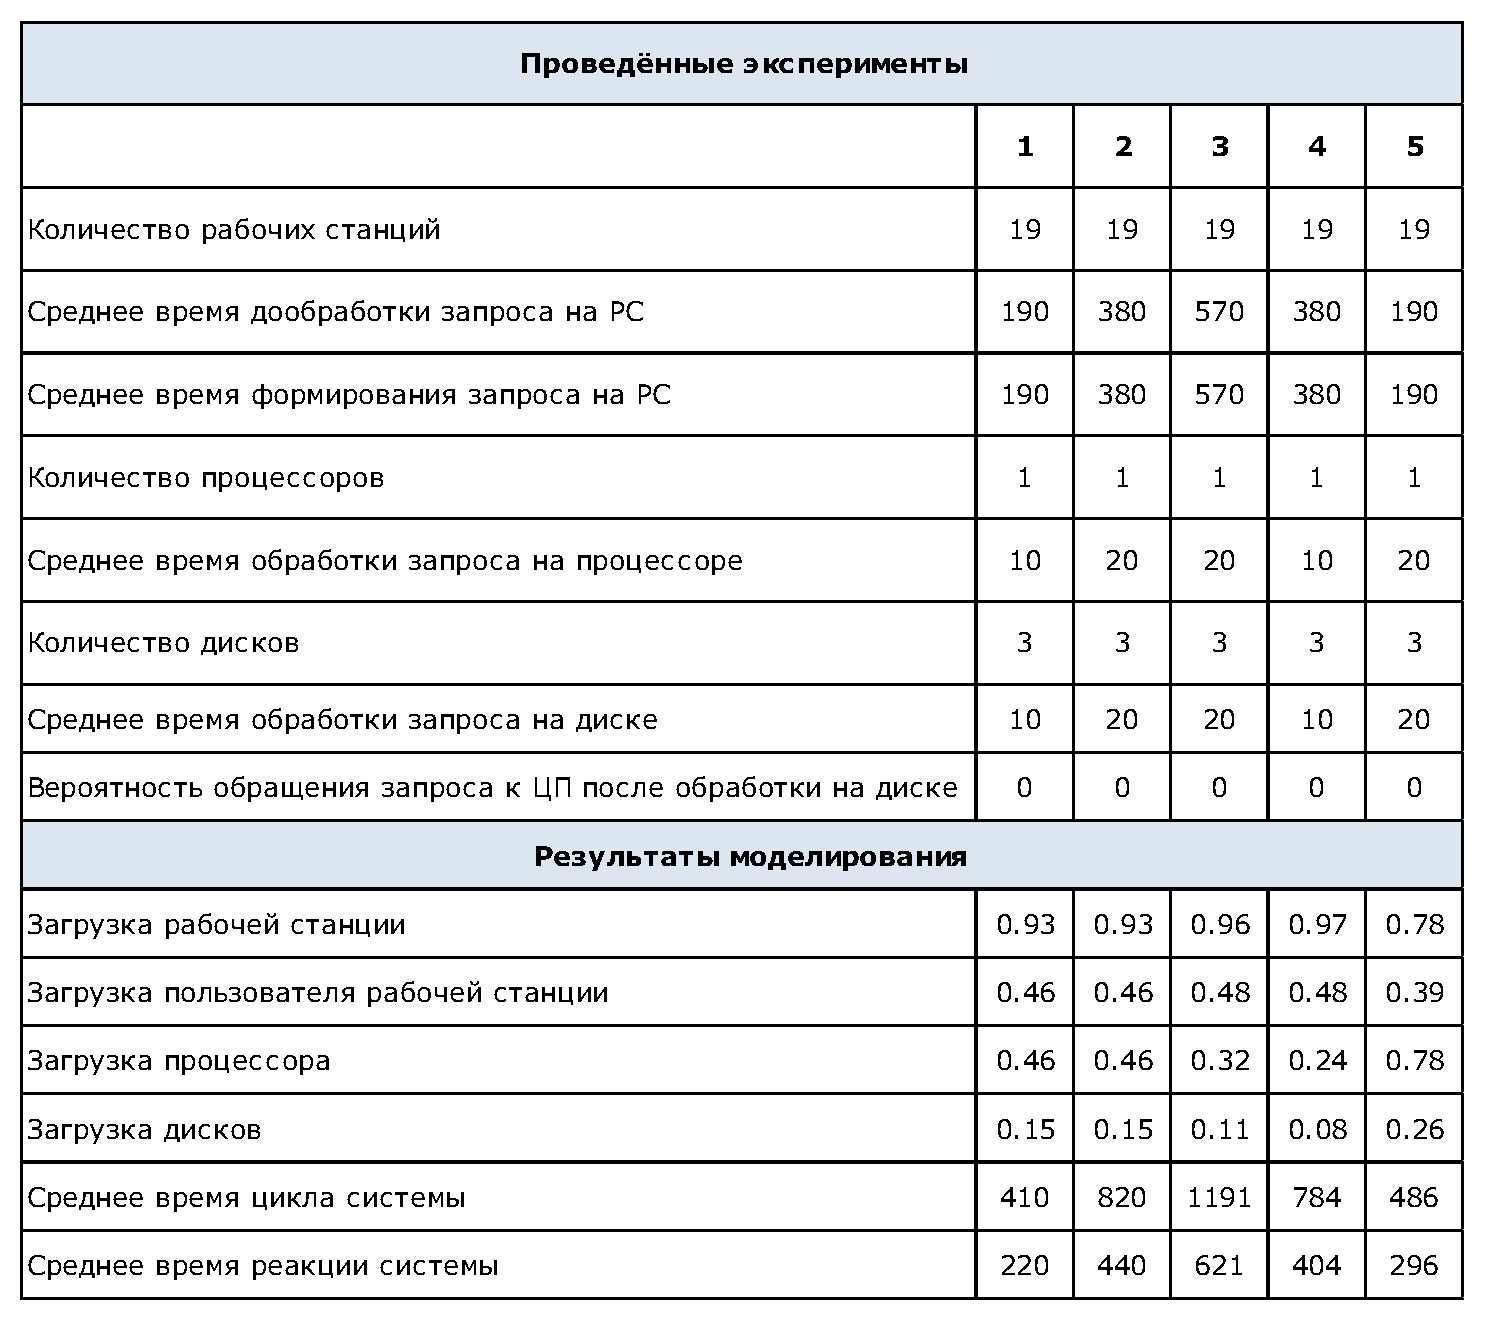
\includegraphics[width=0.7\linewidth]{pics/pic10_1_anal_result.eps}
 \end{tabular}
\end{table}                    % Аналитическое моделирование
%\newpage

\subsection{Имитационное моделирование}

Необходимо выполнить имитационное моделирование рассматриваемой системы средствами языка GPSS.\par\bigskip

Структура программы:\\
\verb|INITIAL| -- блок задания количественных и временных параметров исходных данных моделируемой системы;\\
\verb|STORAGE| -- блок задания многоканальных узлов системы;\\
\verb|FUNCTION| -- блок задания функции распределения запросов по узлам и времени выполнения запросов в узлах;\\
\verb|GENERATE| -- блок генерации количества задач, циркулирующих в системе;\\
\verb|PCF| -- метка, объединяет набор блоков, описывающих формирование запроса на рабочей станции;\\
\verb|CAN| -- метка, объединяет набор блоков, описывающих обработку эапроса в канале;\\
\verb|SRV| -- метка, объединяет набор блоков, описывающих обработку эапроса в процессоре;\\
\verb|PER| -- метка, объединяет набор блоков, описывающих правило перехода запроса после обработки на диске в канал;\\
\verb|PCD| -- метка, объединяет набор блоков, описывающих дообработку запроса на рабочей станции.\par\bigskip

Текст программы на языке GPSS:
\begin{verbatim}
INITIAL X$STATION_N,19   ; количество рабочих станций
INITIAL X$STATION_TD,190 ; время на дообработку запроса
INITIAL X$STATION_TF,190 ; время на формирование запроса
INITIAL X$CPU_T,20       ; время обработки процессором
INITIAL X$DISK_N,3       ; количество дисков
INITIAL X$DISK_T,20      ; время обработки на диске
;INITIAL X$CANAL_T,5

FLAG1 VARIABLE 0
FLAG2 VARIABLE 1

WORKSTATION_D  STORAGE 19
WORKSTATION_F  STORAGE 19
WORKSTATION_PC STORAGE 19
CPU            STORAGE 1

DISK_N FUNCTION RN1,D2
0.5,1/1,2

EXPON               FUNCTION                RN1,C23
0,0/.1,.104/.2,.222/.3,.355/.4,.510/.5,.69/.6,.915/
.7,1.2/.75,1.37/.8,1.5/.84,1.83/.88,2.12/.9,2.3/
.92,2.52/.94,2.82/.95,2.98/.96,3.2/.97,3.5/.98,3.9/
.995,5.3/.998,6.2/.9995,7/1,8

GENERATE ,,,X$STATION_N
ASSIGN FLAG1,V$FLAG1
ASSIGN FLAG2,V$FLAG2

PCF QUEUE   QSYSTEM
    QUEUE   QREACTION
    ENTER   WORKSTATION_F,1
    ADVANCE X$STATION_TF,FN$EXPON
    LEAVE   WORKSTATION_F,1
    ASSIGN  3,SRV
    TEST E  P$FLAG1,P$FLAG2,CAN
    LEAVE   WORKSTATION_PC,1

;CAN QUEUE   QCANAL
    ;SEIZE   CANAL
    ;DEPART  QCANAL
    ;ADVANCE X$CANAL_T,FN$EXPON
    ;RELEASE CANAL
CAN TRANSFER ,P3

SRV QUEUE    QCPU
    ENTER    CPU,1
    ADVANCE  X$CPU_T,FN$EXPON
    LEAVE    CPU,1
    DEPART   QCPU
    ASSIGN   5,FN$DISK_N
    QUEUE    P5
    SEIZE    P5
    DEPART   P5
    ADVANCE  X$DISK_T,FN$EXPON
    RELEASE  P5
    TRANSFER 0.0, PER,SRV

PER ASSIGN   3,PCD
    TRANSFER ,CAN

PCD DEPART   QREACTION
    ENTER    WORKSTATION_PC,1
    ENTER    WORKSTATION_D,1
    ADVANCE  X$STATION_TD,FN$EXPON
    LEAVE    WORKSTATION_D,1
    DEPART   QSYSTEM
    ASSIGN   FLAG1,1
    TRANSFER ,PCF

    GENERATE  100000
    TERMINATE 1
    START     1
\end{verbatim}

Так как канал в рассматриваемом варианте модели отсутствует, то соответствующие строки закомментированы.\par\bigskip

\newpage

Результаты имитационного моделирования представлены в таблице~\ref{table:imit_result}.

\begin{table}[h]
\caption{Результаты имитационного моделирования}
\label{table:imit_result}
\centering
 \begin{tabular}{c}
 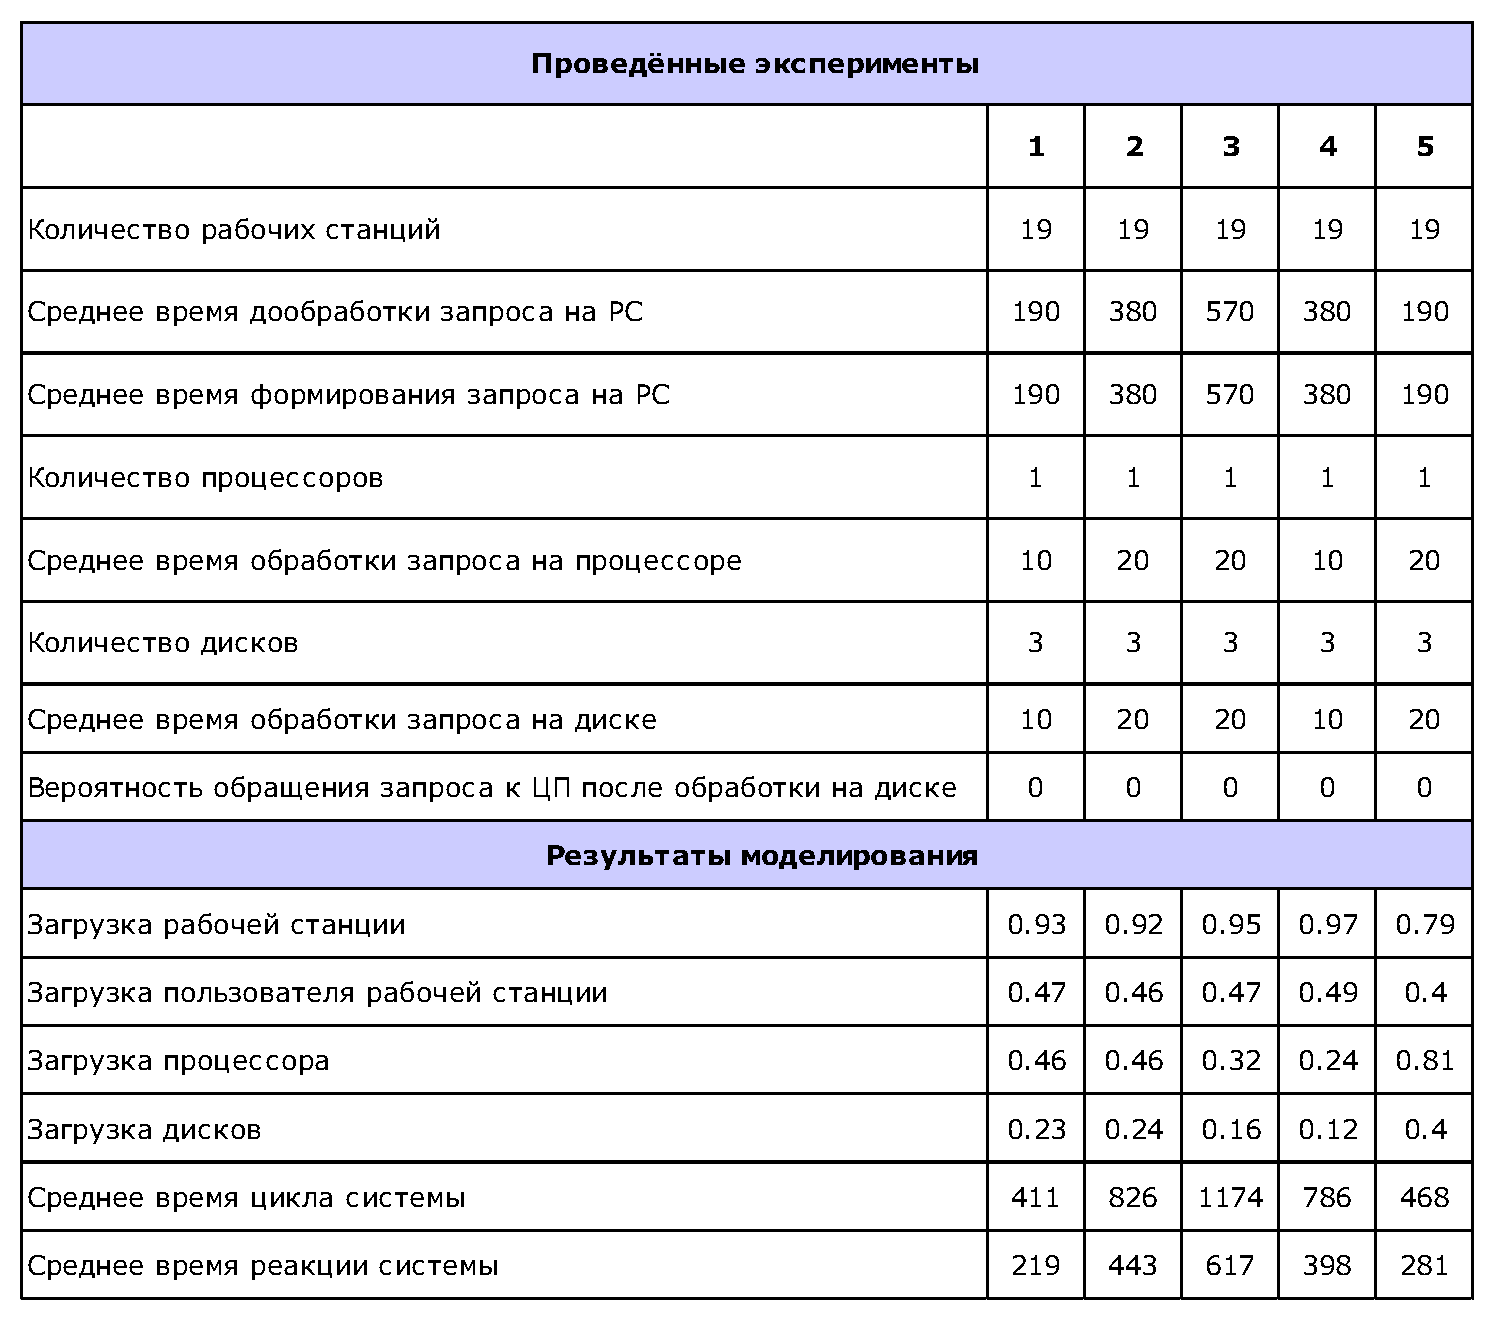
\includegraphics[width=0.7\linewidth]{pics/pic11_1_imit_result.eps}
 \end{tabular}
\end{table}                  % Имитационное моделирование
%\newpage

\subsection{Сравнительный анализ результатов моделирования}

Сравнение результатов аналитического и имитационного моделирования приведено ниже в таблице~\ref{table:result_compr}.

\begin{table}[h]
\caption{Сравнение аналитического и имитационного моделирования}
\label{table:result_compr}
\centering
 \begin{tabular}{c}
 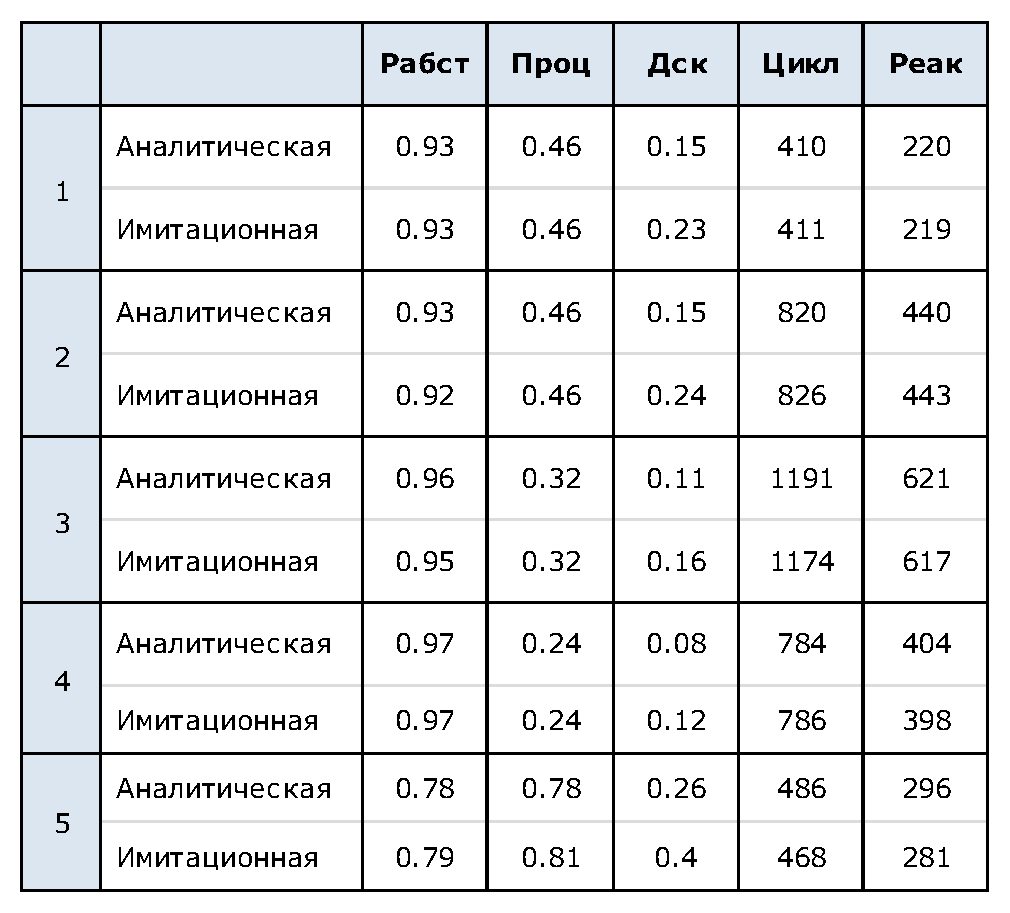
\includegraphics[width=0.7\linewidth]{pics/pic12_1_result_compr.eps}
 \end{tabular}
\end{table}

Сравнительный анализ приведенных результатов показывает, что различие между результатами аналитического и имитационного моделирования составляет не более 10\%. Это вполне приемлемый для инженерных расчётов результаанализ приведенных результатов показывает, что различие между результатами аналитического и имитационного моделирования составляет не более 10\%. Это вполне приемлемый для инженерных расчётов результат.\par\bigskip

Разница в значениях между аналитическим и имитационным моделированием объясняется следующими причинами:
\begin{itemize}
\item при аналитическом моделировании методом фонового потока использовали приближённый итерационный алгоритм нахождения значений выходных характеристик рассматриваемой системы;
\item при имитационном моделировании на языке GPSS задавали ограниченное время моделирования и использовали приближенную экспоненциальную функцию распределения времени обслуживания, которую задавали по точкам.
\end{itemize}                        % Сравнение результатов
%\newpage

\section{Выводы}

В данной работе было разработано проектное решение на построение распределённой АСОИиУ фирмы и получены следующие результаты:
\begin{itemize}
\item выбрана структура сетей для центрального офиса и филиалов в соответствии с заданными параметрами;
\item построена блок-схема сети и структурные схемы ЛВС центрального и удаленных офисов;
\item описаны правила построения сетей фирмы;
\item для удаленной связи офисов была выбрана технология ADSL, как наиболее подходящая под выбранные задачи;
\item произведено сравнение оборудования разных производителей и выбран оптимальный вариант;
\item приведены методы увеличения производительности и отказоустойчивости серверов;
\item описана настройка рабочих параметров сетевой ОС MS Windows 7;
\item описана настройка рабочих параметров СУБД Sybase;
\item выполнено распределение предметных баз данных по узлам сети;
\item произведено аналитическое и имитационное моделирование функционирования ЛВС с последующим сравнением полученных результатов.
\end{itemize}                       % Выводы
%\newpage

\section{Литература}

\begin{enumerate}
\item Методические  указания к курсовой работе по дисциплине "Эксплуатация АСОИиУ";
\item Лекции по курсу "Эксплуатация АСОИУ";
\item Галкин В.А., Григорьев Ю.А. - "Телекоммуникации и сети";
\item Чёрненький В.М. - Учебное пособие по GPSS.
\end{enumerate}                         % Литература

%\addcontentsline{toc}{chapter}{\bibname}
\bibliographystyle{utf8gost705u}
\bibliography{biblio}

\end{document}